\documentclass[a4paper,12pt,twoside]{book}
\usepackage{upatras-thesis}

% PDF settings
%
% \hypersetup
% {
%     pdfauthor={\me},
%     pdftitle={\shortdoctitle},
%     pdfsubject={\doctitle},
%     pdfkeywords={\keywords},
%     pdfproducer={pdfLaTeX},
%     pdfcreator={\creator}
% }

%
% These commands need to be defined in order to produce a correct and personalized document
%
\newcommand{\shortdoctitle}{Thesis}
\newcommand{\doctitle}{An IoT Edge-as-a-service (Eaas) Distributed Architecture \& Reference Implementation}
% \newcommand{\docsubtitle}{Υπότιτλος εγγράφου}
\newcommand{\division}{Electronics and Computers Department}
\newcommand{\lab}{Network Architectures \& Management group, Applied Electronics Laboratory}

\newcommand{\me}{Odysseas Lamtzidis of George-Patroklos} %(σε γενική πτώση) ΠΡΟΣΟΧΗ: στοιχεία σε γενική πτώση. Παράδειγμα: Άγγελου Σικελιανού του Ιωάννη
%
\newcommand{\nomme}{Odysseas Lamtzidis of George-Patroklos} %(σε ονομαστική πτώση) ΠΡΟΣΟΧΗ: στοιχεία σε ονομαστική πτώση. Παράδειγμα: Άγγελος Σικελιανός του Ιωάννη
%
\newcommand{\studnum}{1019749}
\newcommand{\keywords}{Internet of Things; Blockchain; Edge computing; ;implementation; Sharing Economy}
\newcommand{\monthyear}{September 2019}

\newcommand{\supname}{Dr. John Gialelis}
\newcommand{\suptitle}{EDiP}
\newcommand{\supuni}{University of Patras}

\newcommand{\cosupname}{Spyros Denazis}
\newcommand{\cosuptitle}{Associate Professor}
\newcommand{\cosupuni}{University of Patras}

\newcommand{\headofdivision}{Vasileios Paliouras}
\newcommand{\headofdivisiontitle}{Associate Professor}

\author{\me}

% GLOSSARY

\makeglossaries
\setlength{\glsdescwidth}{0.7\hsize}
\setlength{\headheight}{15pt}
\newglossaryentry{iot-connection}
{name=IoT Connection, description={ In the proposed system architecture each child layer is “managed” by the parent layer. A connection indicates this management relationship between two devices (e.g cloud-edge) that belong to different layers.}}
\newglossaryentry{iot-management}
{name=IoT Management, description={IoT Management is a generic term that describes various activities which can range from serving as a gateway to performing data analytics on the streamed data while offering additional services such as a GUI dashboard. These activities and services are offered from a parent device to children device.}}

\newglossaryentry{edge-computing}{
name=Edge Computing,
description={Edge computing is a “mesh network of micro data centers that process or store critical data locally and push all received data to a central data center or cloud storage repository.}}

\newglossaryentry{fault-tolerance}{
    name=Fault-Tolerance,
    description={High availability or Fault-Tolerance references to the ability of a system to continue it’s functionality in the case of a critical failure due to the replication of the services to multiple machines in distributed manner.}
}

\newglossaryentry{stakeholder}{
    name=System Stakeholder,
    description={System Stakeholder or simply Stakeholder is the owner of devices that can belong to one or multiple IoT layers, thus forming a vertical slice. Depending on the use case, the stakeholder can also be the system administrator and infrastructure owner.}
}

\newglossaryentry{system-provider}{
name=System Provider,
description={The system provider is the company that produces and sells the system’s software, while also offering core services, such as the marketplace.}
}

\newglossaryentry{south-side}{
    name=South Side,
    description={All IoT objects, within the physical realm, and the edge of the network that communicates directly with those devices, sensors, actuators, and other IoT objects, and collects the data from them, is known collectively as the “South Side.”}
}
\newglossaryentry{north-side}{
    name=North Side,
    description={The Cloud where data is collected, stored, aggregated, analyzed, and turned into information, and the part of the network that communicates with the Cloud, is referred to as the “north side” of the network.}
}

\newglossaryentry{permission}{
    name=Permission,
    description={ Depending on whether the participant nodes need permission from a central authority to participate in the blockchain and write in the ledger, the network is called permission-less or permissioned. }
}
\newglossaryentry{trust}{
    name=Trust (blockchains),
    description={A blockchain is called trustless, if the protocol allows the network to function even when nodes do not trust each other. Otherwise the blokchchain is called trusted}
    }
\newglossaryentry{microdc}{
name=Micro DataCenter,
description={Micro Data centers are data centers with an exceptionally small number of servers racks that is situated geographically near the location of the users that is serving.}}

\newacronym{iot}{IoT}{Internet of Things}

\newacronym{eaas}{EaaS}{Edge as a Service}

\newacronym{ipfs}{IPFS}{Inter Planetary File System}

\newacronym{os}{OS}{Operation System}

\newacronym{mec}{MEC}{Mobile Edge Communications}

\newacronym{vm}{VM}{Virtual Machine}

\newacronym{mqtt}{MQTT}{Message Queuing Telemetry Transport}

\newacronym{rpc}{RPC}{Remote Procedure Call}

\newacronym{rest}{REST}{REpresentational State Transfer}

\newacronym{api}{API}{Application Program Interface}

\newacronym{m2m}{M2M}{Machine-to-Machine}

\newacronym{pow}{PoW}{Proof of Work}

\newacronym{qos}{QoS}{Quality of Service}

\newacronym{qa}{QA}{Quality Assurance}

\newacronym{dmu}{DMU}{Decission Making Unit}

\newacronym{abp}{ABP}{Activation-by-Personalisation}
% BEGIN DOCUMENT
\begin{document}

% SET PAGE NUMBERING TO ROMAN
\pagenumbering{roman}
\setcounter{page}{3}

%*************************%
%         TITLES          %
%*************************%

\begin{titlepage}
\begin{center}
% Upper part of the page
{\large University of Patras - Polytechnic School}\\
\large Department of Electrical Engineering\\and Computer Technology\\
\hfill \break

\includegraphics[width= 0.8\textwidth]{up_landscape}\\
\hfill \break
{\Large Department: \division \\
Laboratory: \lab }\\[1cm]

{\uline{\LARGE{\shortdoctitle }}}\\ [0.5cm]
of the student of Department of Electrical Engineering\\
and Computer Technology of the Polytechnic School of the University of Patras\\[1cm]

{\LARGE \me }\\[0.5cm]
{\Large record number: \studnum}\\[1cm]

\uline{\large Subject}\\[0.5cm]
\textbf{\large \doctitle }\\[1cm]
\uline{\large Supervisor}\\[0.5cm]
\large \suptitle \, \supname, \supuni \\[1cm]
\large{Thesis Number: }\hspace{3cm}
\vfill
% Bottom of the page
\large{Patras, \monthyear}
\end{center}
\end{titlepage}

\clearemptydoublepage

\pagestyle{empty}
\begin{center}
{\LARGE ΠΙΣΤΟΠΟΙΗΣΗ\\[1cm]}
\large Πιστοποιείται ότι η διπλωματική εργασία με θέμα\\[1cm]
\textbf{\large \doctitle }\\[1cm]
του φοιτητή του Τμήματος Ηλεκτρολόγων Μηχανικών και Τεχνολογίας Υπολογιστών\\[1.5cm]
\me \\[0.5cm]
(Α.Μ.: \studnum )\\[1.5cm]
παρουσιάστηκε δημόσια και εξετάστηκε στο τμήμα  Ηλεκτρολόγων Μηχανικών και Τεχνολογίας Υπολογιστών στις\\[1cm]
\Large{\_\_/\_\_/\_\_\_}\\[1.5cm]
\end{center}
\begin{minipage}{0.5\textwidth}
\begin{flushleft} \large
Ο Επιβλέπων\\[2cm]
\supname \\
\emph{\suptitle}\\[1cm]
Ο Συν-Επιβλέπων\\[2cm]
Σταύρος Κουμπιάς
\newline Professor
\end{flushleft}
\end{minipage}
\begin{minipage}{0.5\textwidth}
\begin{flushright} \large
Ο Διευθυντής του Τομέα\\[4cm]
\headofdivision\\
\emph{\headofdivisiontitle}
\end{flushright}
\end{minipage}

\clearemptydoublepage

\pagestyle{empty}
\begin{center}
{\LARGE CERTIFICATION\\[1cm]}
\large It is certified that the Thesis with Subject\\[1cm]
\textbf{\large \doctitle }\\[1cm]
of the student of the Department of Electrical Engineering \& Computer Technology\\[1.5cm]
\me \\[0.5cm]
(R.N: \studnum )\\[1.5cm]
Was presented publicly and defended at the Department of Electrical Engineering \& Computer Technology at\\[1cm]
\Large{\_\_/\_\_/\_\_\_}\\[1.5cm]
\end{center}
\begin{minipage}{0.5\textwidth}
\begin{flushleft} \large
The Supervisor\\[2cm]
\supname \\
\emph{\suptitle}\\[1cm]
The Co-Supervisor\\[2cm]
Stavros Koubias
\newline Professor

\end{flushleft}
\end{minipage}
\begin{minipage}{0.5\textwidth}
\begin{flushright} \large
The Director of the Division\\[4cm]
\headofdivision\\
\emph{\headofdivisiontitle}
\end{flushright}
\end{minipage}

\clearemptydoublepage

\pagestyle{empty}
\hspace{10pt}
\begin{center}
\Large{Thesis details}\\[1cm]
{\large Subject:}
\textbf{\large \doctitle}\\[1cm]
\large {Student: \textbf{\nomme}\\[1cm]
\large{Supervising Team}\\
\textbf{\suptitle \, \supname , \supuni}\\[1cm]
\textbf{\cosuptitle \, \cosupname , \cosupuni} \\[1cm]
Laboratories:\\
\lab \\[1cm]
Thesis research period:\\ September 2018 - September 2019\\[1cm]}
\end{center}

\vspace{5em}

\begin{center}
  { \large
    This thesis was written in \LaTeX.\\
  }
\end{center}


\clearemptydoublepage

\pagestyle{plain}
\begin{center}
{\LARGE Abstract}\\[1cm]
\end{center}

Internet of Things (IoT) is an enabling technology for numerous domains worldwide, such as smart cities, manufacturing, logistics and critical infrastructure. On top of Internet of Things, the architectural paradigm shifts from  cloud-centric to Edge-centric, offloading more and more functionality from the cloud to the Edge devices. Edge computing devices are transformed from simply aggregating data to performing data processing and decision making, accelerating the decentralization of the IoT domain. Given the considerable increase of the number of IoT devices and the size of the generated data, an increase of Edge devices with augmented functionality is expected. We propose an "Edge as a service" scheme, where Edge devices will be able to procure unused resources and run services that are requested and consumed by IoT devices that belong to different stakeholders. In this work, we outline a high-level architecture of this scheme and give a reference implementation of a narrow part of the system, boasting high modularity and the extensive use of Open Source Technologies.
 
\clearemptydoublepage

\begin{center}
{\LARGE Acknowledgements}\\[1cm]
\end{center}

I would like to thank, first and foremost, Christos Tranoris, Researcher at the NAM group, who guided me at every step of the thesis, put up with incoherent messages and ideas during the most improper hours. I have the privilege to call him a mentor, a colleague a and a friend. I would also like to thank Professor Spiros Denazis for introducing me to the NAM group and for his insightful comments on this work. Most importantly, I want to thank John Gialelis who introduced me to the  world of Academic Research and who has been my mentor for over 2 years. Finally, I want to thank the whole team of NAM group for the fruitful conversations, as also the online communities and developers of the projects: \textit{EdgeX Foundry}, \textit{Filecoin}, \textit{loraserver.io}, \textit{Node-RED} and \textit{balena}, for their continuing assistance and guidance throughout the implementation. I dedicate this work to my Parents, \textit{Despoina} and \textit{George}, who laid the foundations for everything I have accomplished thus far, and to my friends and my companion, who have supported me, put up with me and pushed me to become a better human being.

\clearemptydoublepage

\pagestyle{empty}

{\hypersetup{linkcolor=black}
\tableofcontents
}
\clearemptydoublepage

%*************************%
%    1. Lists of figures  %
%    2. List of Tables    %
%    3. Glossary          %
%*************************%
% \listoffigures
% \listoftables
% \printglossaries
% \clearemptydoublepage

{\hypersetup{linkcolor=black}
\listoffigures
\listoftables
}
\glsaddall
\printglossary[style = mylong]
\printglossary[type=acronym,style=custom_acronyms]
\clearemptydoublepage
% \gamo_ton_xristo_sou_glossary
% easter_egg

\mainmatter % book mode only
\clearemptydoublepage


\pagestyle{fancy}
\pagenumbering{arabic}
\setcounter{page}{1}

%*************************%
%       Main Chapters     %
%*************************%

% Introduction
%!TEX root = ../main.tex

\chapter{Introduction}
\markboth{Introduction}{}
%\vspace{-1.3in}

\paragraph{}
The Internet of Things refers to a relevantly new industry, which features the interconnection of every physical object with each other, using the internet as the bedrock for such a connection. In the era of Internet of Things, data is gathered from a myriad of sources in order to be processed and converted into wisdom, knowledge that will enables us to make smarter decisions in our everyday lives, in the planning of our cities and even in the damage control of natural disasters. Internet of Things is truly a frontier that will play a key role in the following years in a vast array of industries and domains.

\section{Reference Architecture}
The Internet of Things reference architecture, according to Cisco, can be summarised in Figure \ref{fig:iotarchsisco}, where there are 7 distinct layers of different activities that are conducted in a vertical slice of a typical Internet of Things system. The vertical slice refers to the fact that the system incorporates all 3 tiers of the systems (Constrained Devices or “Things", Edge, Cloud).  Throughout this thesis,  we will quote the various sensors, cameras, servos or even microcontrollers (like Arduino)  and other arbitrary \acrfull{iot} devices as “Constrained Devices”, in the sense that they have a very narrowly focused function and limited processing capability (if any).  While the typical architecture implies that layer 1 is at the “Things” tier, layers 2 and 3 at the Edge tier and layer 4 to 7 at the Cloud tier, the Edge computing paradigm pushes functionality from layer 4 to 7 down to layer 3.

\begin{figure}[h]
    \centering
    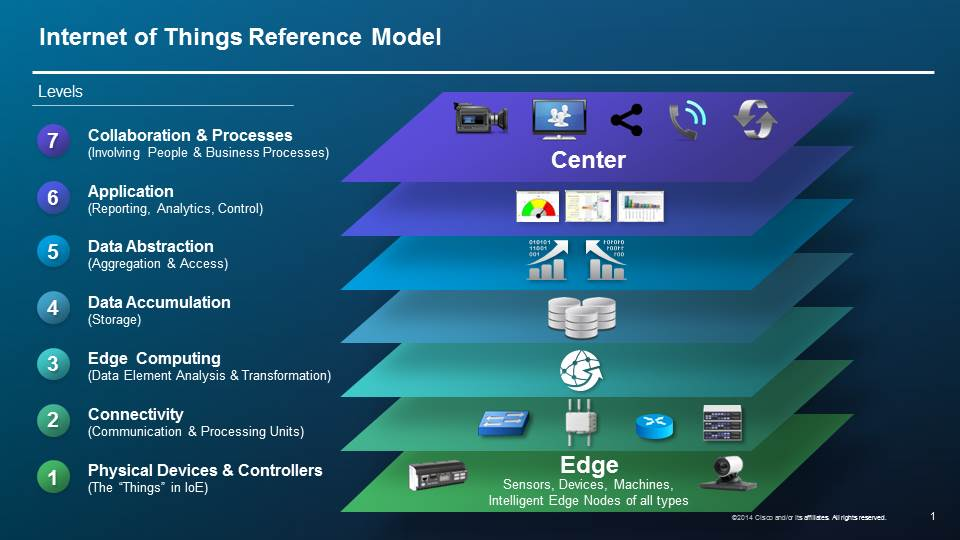
\includegraphics[width=\textwidth]{images/iotArchCisco.jpg}
    \caption{Illustration of the IoT Reference Model by Cisco\cite{iot-reference}}
    \label{fig:iotarchsisco}
\end{figure}

In terms of physical machines, a typical IoT hierarchical structure can be viewed in Figure \ref{fig:hier_arch_primer}, where the fog nodes communicate both with the cloud and with other fog nodes, either wirelessly or by wire.  Fog nodes can also function in a layered fashion, performing a different functionality according to their proximity to the data generators, which is still much closer than the cloud. Near the data source, fog nodes are mainly positioned in order to aggregate data, perform semantic notation and control the various actuators. Actuators are simply constrained devices that can interact with the physical world (e.g servos). Fog nodes that are upwards could perform more abstract functions, such as turning raw data into knowledge via processing. In this example, fog nodes can even be a non-homogenous group, even for the same stakeholder and system, as nodes closer to the source could be lighter in terms of processing and power consumption, such as the Raspberry pi \cite{rpi3}, while fog nodes that perform the bulk of pre-processing would be akin to a  \gls{microdc}(μDC).


\begin{figure}[h]
    \centering
    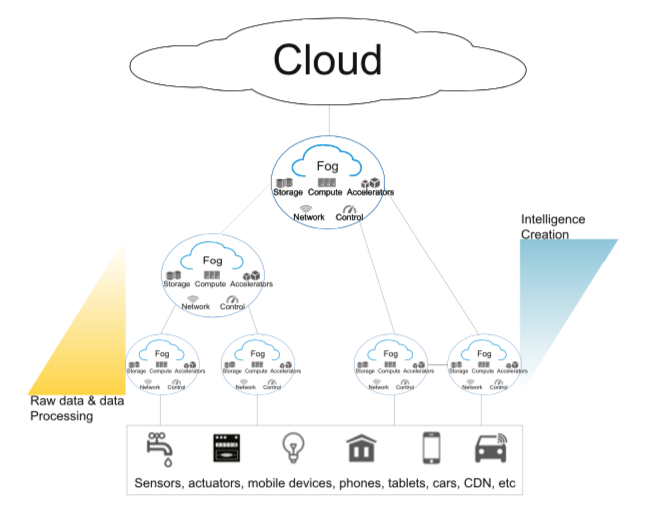
\includegraphics[width=\textwidth]{images/hierarchichal_architecture(from-primer).png}
    \caption{The hierarchical architecture of multiple fog computing layers\cite{ai2018edge} }
    \label{fig:hier_arch_primer}
\end{figure}

\section{Fog Computing}
The fog paradigm or more commonly known, \gls{edge-computing},  proposes that a part of the system’s intelligence and functionality must be implemented near the data source as opposed to the cloud-centric approach. While the terms“edge” and “fog” are commonly used interchangeably, the reader should be aware of the distinctions, especially when overviewing relevant bibliography. 

Edge computing refers to the concept of bringing resources closer to the data source, while fog computing was introduced by Cisco in 2014 as a terminology to define the edge computing as a standard\cite{linthicum2019}.  Edge computing has increased in popularity due to the fact that computational resources are becoming cheaper while the amount of data generated by devices is growing at an never before seen speed\cite{ericsson}. The placement of IoT resources with increasingly distributed architectures can be seen as akin to the evolution of the Internet, as at its beginnings, the mainframes were few and owned by trusted authorities (government, universities, etc.)\cite{leiner2009brief}. With the proliferation of the technology, we saw a democratization of the platform and an exponential increase in smaller servers with many different private stakeholders. 

The objective of the edge is to perform low-latency computation and some pre-processing on the raw data before sending them to the cloud. It offers a massive decrease of network costs since only a fraction of the data is actually transmitted to the cloud, offering at the same time, superior services to the consumers since the processing and decision making is happening near the source. These characteristics, can become even apparent, given the numbers of data throughput in modern applications. A boeing 787 generates about 5 GB of data per second, data that needs processing and which is highly sensitive, both in nature and decision making impact \cite{datafloq}. Another interesting example is an autonomous vehicle, which generate about 1GB of data \cite{finnegan2013}per second, data that need real time processing and decision making. This need for extreme low-latency can simply not be supported by a cloud solution, both in terms of network latency and scalability. We would need a cloud computing system that should be able to support effortlessly millions of cars (thus GB/s) while offering extreme low response time, something that at the moment is not technologically feasible.


\section{ The Edge computing paradigm in the Internet of Things}

On top of the above examples, if we narrow down the Edge Computing paradigm at the Internet of things, the case rests unchanged. Taking into consideration the increasing number of smart devices, such as smart-home (LED bulbs, speakers, home-automation, etc.) a cloud centric solution will not be able to cope with the amount of data \& processing needed, even if it is not as time critical as the examples above. A survey by Sony Ericsson indicates that by 2022 we could have 18 billion connected IoT devices\cite{ericsson}. 

Thus, the development of the IoT Edge Computing paradigm seems imperative in order to create the infrastructure needed to support this ecosystem. Figure \ref{fig:fog_comp_app} shows a sample of the many applications that exist for the Internet of things. The outermost layer of the image is populated by the constrained devices that have a specialised function over a a domain (e.g Power Supply), while the middle layer is populated of the Edge Nodes and finally, the innermost consists of the cloud that manages the inner layers and offers additional services (e.g long-term storage). It is interesting to comment that not only the number of distinct devices is reduced as we advance to the center of the cycle, but also, as we advance the homogeneity of the systems is increased. Constrained devices are highly specialized and thus numerous is numbers and in forms, while a datacenter can host all kinds of different applications, which of course share certain similarities (i.e they share certain elements, such as domain, stakeholder, critical factor).

In this thesis, we outline the architecture and main characteristics of an Internet of Things system that follows the Edge computing paradigm, with emphasis on data integrity and high availability. We will focus our architectural design \& implementation on the fog tier of the IoT stack, creating a layer that is agnostic both in terms of Constrained Devices and Cloud backend infrastructure. Our proposed architecture has the following key characteristics:
\begin{itemize}
 \item it is built on top of the microservices paradigm for extensive modularity and expandability
  \item it is based almost entirely on open source projects, so that we are able to contribute and showcase their incredible potential
 \item it exploits the unique characteristics of the container technology that is commonly used in cloud environments but modified for the needs and characteristics of the Edge.
 \item a novel blockchain based technology is used to store both the available application logic and data, in an effort to provide data integrity across the pipeline and facilitate  the high availability of the platform
\item the implementation is based on a Raspberry pi 3 micro-computer where we will attempt the dynamic handover of LoRa devices, between devices that belong to different stakeholders and have, perhaps, different functionality.
\end{itemize}

\begin{figure}[h]
    \centering
    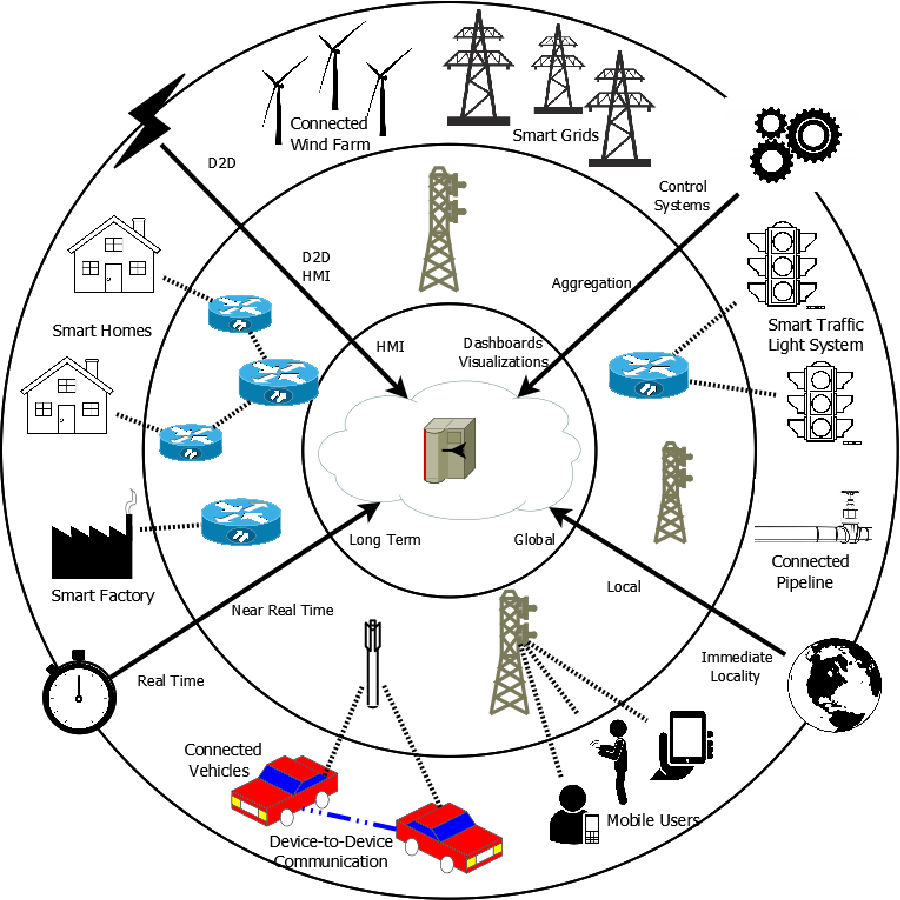
\includegraphics[width=0.7\textwidth]{images/fogComputingApplications(from-principles).png}
    \caption{The Internet of Things is relevant to an array of different domains\cite{dastjerdi2016fog}}
    \label{fig:fog_comp_app}
\end{figure}

Our proposed  Edge platform and prototype implementation, enables the Edge provider to dynamically execute applications and services demanded by clients,  “renting”, in essence, a part of their Edge Infrastructure to perform the application logic of a 3rd party. Enabling thus, the concept of \textbf{“IoT Edge computing as a Service”}, where the Edge Resources are actively offered and demanded in an IoT Edge Computing Marketplace. In this context, we outline a use-case in the domain of \gls{fault-tolerance}, where an Edge Node faces a critical failure and handovers its sensors and its services to another pre-determined Edge Node.

In Chapter \ref{ch:problem-statement} we underline the problem statement of this thesis and the state of art solutions that exist, in Chapter \ref{ch:system-architecture} we introduce the high level architecture while in Chapter \ref{ch:implementation} we give a proof of concept implementation in the form of a walkthrough tutorial. Finally in Chapter \ref{ch:discussion} there is a discussion on the various aspects of the implementation and our assumptions, in Chapter \ref{ch:results} we conclude with the results of this work and in Chapter \ref{ch:future-work} we talk about future work on this research vertical.

\clearemptydoublepage

% Chapter 1
 \chapter{Problem statement- State of the art} \label{ch:problem-statement}
\markboth{Problem statement- State of the art}{}

\paragraph{}
The key idea of this thesis is  an architecture that enables the implementation of economically attractive solutions that offer High-Availability to the IoT Edge Layer. It also proposes the most optimum way for critical infrastructure to be fault-tolerant, both in terms of services/functionality but also in terms of data quality (data integrity). However, preliminary discussions with experts of the domain (e.g. balena, EdgeX, blockchain domain)   led us to a more generic approach: That of resource sharing in a concept of share economy, in the domain of IoT Edge resources.

\section{The Sharing Economy}

Sharing Economy or “gig” economy is a relatively new term \cite{sharingeconomy},  popularised by famous companies like Airbnb or Uber. The idea is that services and goods can be distributed in a decentralized fashion, not by companies with employees but by private individuals who rent currently unused resources to other private individuals in a peer to peer fashion. In the above mentioned examples, individuals can rent their house (or part of it) when they don’t use it (Airbnb), or rent the “unused” seats of their cars, working, in essence, as taxi drivers whenever they choose to (e.g Uber, Lyft, etc.). Figure \ref{fig:sharing_economy} illustrates the concept of “Sharing Economy” for Airbnb which in essence provides access to Market to both parties of the value chain (Demand, Offer).

\begin{figure}[h]
    \centering
    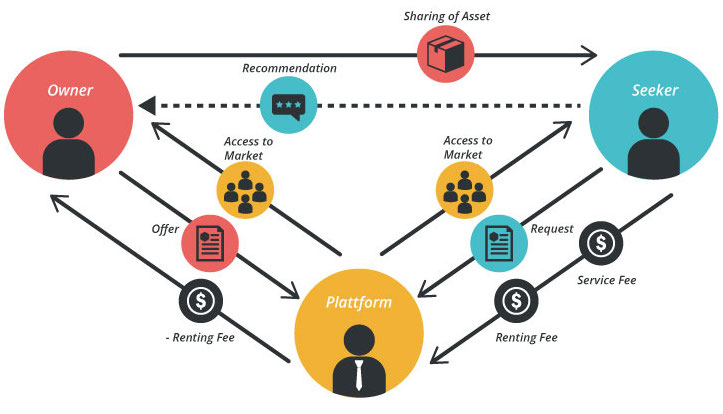
\includegraphics[width=0.9\textwidth]{images/sharingEconomy.jpg}
    \caption{The Sharing Economy Model;use-case of Airbnb\cite{airbnb}}
    \label{fig:sharing_economy}
\end{figure}

\section{Sharing Economy in the Internet of Things?}

We now attempt to apply the principles outlined in the above examples to the domain of IoT Edge resources.By tapping into that notion, IoT edge nodes could in fact share resources in order to provide services one to another, without necessarily belonging to the same stakeholder or even forming a federation. By incentivizing the IoT Edge Nodes to share resources, with a currency of sorts, we can foresee a \acrfull{m2m} marketplace, where IoT Edge Nodes will dynamically rent the resources that they need. In this scenario, an IoT Edge Node could provide Fault - Tolerance capabilities to nodes that are willing to pay for them. This could lead to a much more sustainable path of proliferating IoT Edge Computing , since it can considerably reduce the upkeep cost. There is no sense in owning Resources that you don’t use, only to anticipate a spike or an exception in the normal activity, but rather you can rent ad-hoc that extra computational power, if ever there is a need for it.

Indeed, the principle can be expanded with not only conventional computing resources, which we will define in Section \ref{st:edge-resources}  , but even with IoT specific “resources”. We argue that the handling of constrained devices (provision, management, data aggregation, semantic notation, metadata addition) can be viewed as a resource to be rented. Dynamic handover of Constrained Devices is an example of IoT specific “resources” that would provide value in a Fault-Tolerance scenario, as the Edge will not only need to take up any processing or decision making, but will also need to handle the data generators for a seamless transition from abnormal to normal operation. In essence, we envision 3rd party applications and/or services to run on the same physical Edge device. This physical Edge device will provide the needed resources to those applications so that they perform their tasks.

It is important here to underline that our solution is not about a multi-tenant platform, where different applications from different parties run on the same hardware. Each edge hardware is owned and operated by a distinct entity (an IoT platform provider for example), which is able to procure some resources to other parties so that they run a part (or even the entirety) of their application logic on the hardware. It is a dynamic relationship that can change rapidly due to the marketplace foundation and the open-ended offer and demand of resources (free market).

In other words, we believe that a platform for IoT Edge Computing as a service, is a much more interesting approach, while Fault - Tolerance is only a use case for it. It is interesting to note that there is not much bibliography concerning the high availability of edge computational resources by sharing them in a p2p economy, other than conventional methods such as backup systems. 

\section{MEC framework}

This idea has already been explored in the \acrfull{mec} framework\cite{7574435} which is believed to be critical for the introduction of 5G networks. Interestingly, while 4G is focused on delivering video content, 5G will focus on the growing M2M connections that is a direct result of the increase of IoT traffic and services\cite{cisco-visualise}. MEC offers cloud-computing capabilities in the RAN environment (Radio Access Network) while also offering an information technology service environment at the edge. They are characterized by very low latency, increased bandwidth and real-time access to radio networks. Moreover-and this is the part that is of interest to us- operators can open their RAN edge to authorized stakeholders so they can deploy their own applications and services toward their own subscribers (i.e private, enterprises and vertical solutions). MEC launched in 2014 by the European Telecommunications Standards Institute MEC Industry Specification Group (ISG) which by the time of writing has finished its work regarding the reference architecture for MEC.

\begin{figure}[ht]
    \centering
    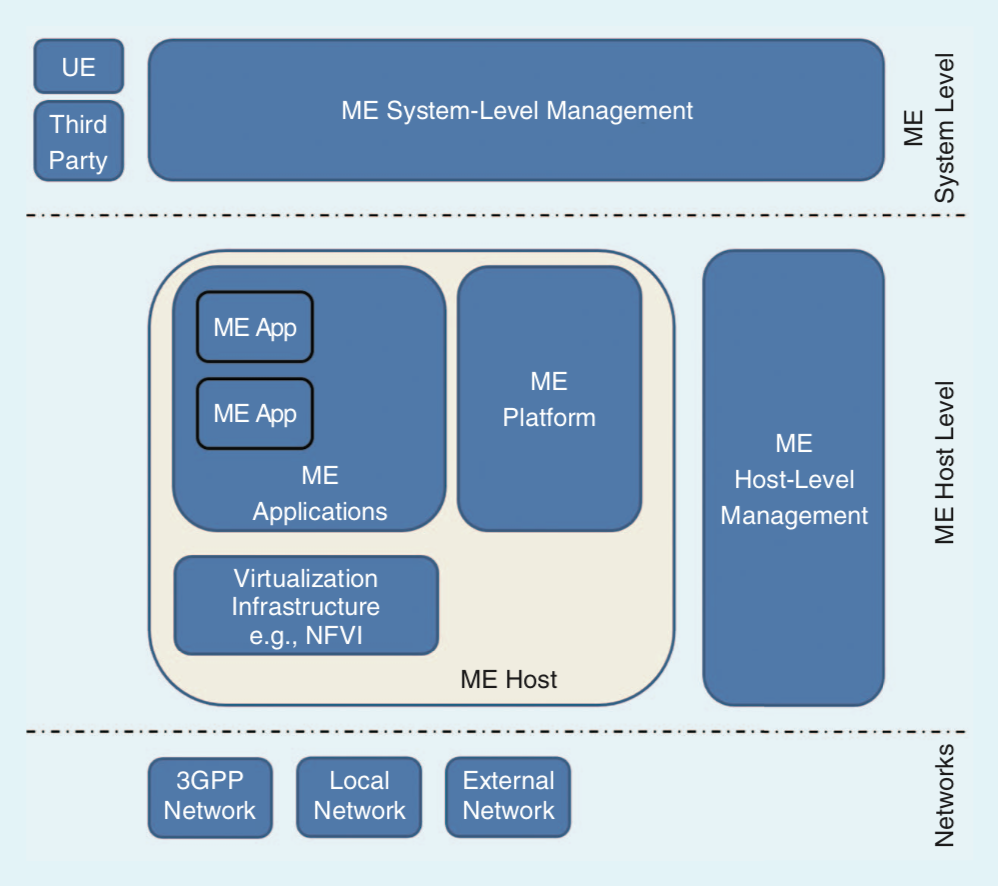
\includegraphics[width=0.9\textwidth]{images/mecarch.png}
    \caption{The High-Level Architecture of the MEC framework\cite{7574435}}
    \label{fig:mec}
\end{figure}

Figure \ref{fig:mec} illustrates the outline of the MEC reference architecture, where the top layer is the whole-system management layer that has an overall visibility of the system, while the bottom layer consists of the connectivity layer which includes all the possible connectivity protocols, from local area networks (LAN) to cellular internet. The layer in between, the host level features the ME platform and applications module, while also the virtualization environment on top of which the applications run. The ME platform is responsible for procuring to the ME applications, all the necessary resources and services they need, MEC can be seen as a cloud server running at the edge of a mobile network.

While MEC is extremely relevant to our solution and a cutting edge piece of standardized software, it diverges significantly from what we are proposing as it assumes trust between the MEC host and the MEC applications. Moreover, it is not designed for a dynamic supply and demand of Edge IoT Resources but rather for more longstanding federation agreements.  Finally, it is important to note that MEC was designed with telecommunications providers in mind, tailoring the architecture to their unique characteristics. Although more diverse deployments are discussed in MEC bibliography, it remains to see their actual effectiveness in regards to the private small-scale provider.

It is important to note that as the research continues on the solution, it is possible that the technology stack will swift to use MEC as the standardisation will improve the quality of the end result.


\section{Edge Resources} \label{st:edge-resources}

According to Mohammad Aazam et al.\cite{aazam2015dynamic} where they illustrate a dynamic resource provisioning mechanism for micro datacenters, computational resources are modeled by a set with the following elements \textit{R = [ CPU, storage, memory, bandwidth]}. In this research work, we will enrich the definition of Edge Resource with a superset of \textit{R}, \textit{R’ = [R, connectivity interface, uptime, battery power]}. This addition of two resources was necessary to model services that demand cyber physical I/O, as for example the handover of bluetooth sensors. The service-provider , apart from apparent CPU, memory \& storage resources, must also “spend” a bluetooth interface of the device. Depending on the use case, battery power or uptime could be an extremely valuable resource. In this context, uptime is defined as the total amount of time that the service will "run" (and which the service provider must ensure the \acrshort{qos}).

Note that the estimation, procurement , management and the monetary evaluation of resources is beyond the scope of this thesis. Nevertheless, the reader will find the above definition of an Edge Resource enlightening, as we dive into the architecture and implementation, in order to better grasp the positioning of our solution. 

Regarding resource management, there are works for efficient scheduling and adaptive offloading schemes that reduce complexity\cite{feng2017ave} with application to autonomous vehicles. Most researchers focus on the optimization of load distribution in a homogenous network of edge nodes that can work collaboratively and  can share the computational load. An example is Rogers Owen et al.\cite{rogers2012financial}, who present a methodology for resource allocation amongst Cloud computers (without resource prediction) while Deelman et al. present trade offs and performance metrics for various resource provisioning plans.  Zhen Xiao et al.\cite{xiao2012dynamic} present a resource allocation system that exploits virtualization technology in order to provision resources to services according to their needs, a vastly different model since it is apparent that it refers to the same physical Edge Node.

\section{ Fault-Tolerance/High-Availability}

High availability or Fault-Tolerance is a common cloud terminology and references to the ability of a system to continue it’s functionality in the case of a critical failure due to the replication of the services to multiple machines in distributed manner. While system redundancy has been partially solved by architectures such as the multi-region architecture, these solutions apply only to the cloud layer and usually the physical mainframes belong to the same stakeholder.

Our research has indicated that fault-tolerance at the edge layer is indeed a new concept, since the edge rarely performed any critical functionality, apart from aggregating sensor data and forwarding them to the cloud. A research study by D. LeClair et al. suggested that Edge Computing availability should surpass that of a data center(99.9\%) and should support at least five nines (99.999\%) availability\cite{ismail2015evaluation}.

Sudip Misra et al. propose an algorithm for fault-tolerance of IoT devices, regarding the routing of the IoT devices, using a Learning Automata as the core of the proposed algorithm \cite{misra2012adaptive}. Bukhary Ikhwan Ismail et al. propose a scheme utilizing the docker container technology as an Edge Computing (EC) platform, meeting a list of requirements that they defined as necessary: 1) deployment and termination; 2) resource \& service management; 3) fault tolerance and 4)caching \cite{ismail2015evaluation}.  The container technology  is in fact part of our solution as mentioned in Architecture Chapter \ref{ch:system-architecture}, but it’s only part of the solution, since the writers use docker swarm and a local docker image registry for each group of edge nodes. This creates multiple “single” points of failure, since a fail-over of the registry can result to the inability of the system to load new images. Details regarding the container technology and an in depth explanation will be given in Section \ref{st:containers}.

Such approaches are inherently different from our proposal since we will be targeting a broader spectrum of Edge devices, where trust between the actors (devices) is not a prerequisite. Our approach is closer to the architecture and principles of Helium \cite{helium}, a startup company which aims to create a decentralized network where nodes are compensated for providing Long Range Network Bandwidth to any sensor interested, as shown in Figure \ref{fig:helium}. The idea is to replicate the model of The Things Network\cite{ttn}, where people contribute their LoRa gateway to the network for anyone to use, but with the addition of an economic incentive to do so. Moreover, they use another communication protocol, called LongFi\cite{gemmell-2019}, a bi-directional data transfer system that is closely related to LoRa in terms of specifications (long range, low bandwidth). On top of it, the system is decentralized, meaning that the network is able to reach a consensus on who is actually providing wireless network coverage without depending on a centralized authority. Our work was greatly influenced by Helium, as network coverage could indeed be one of the resources that our architecture will be able to procure. An example, would be an Edge Device, that provides the activities of data aggregation and north-side forwarding, to any Constraint Device that is interested to pay for them (i.e as-a-service).

\begin{figure}[h]
    \centering
    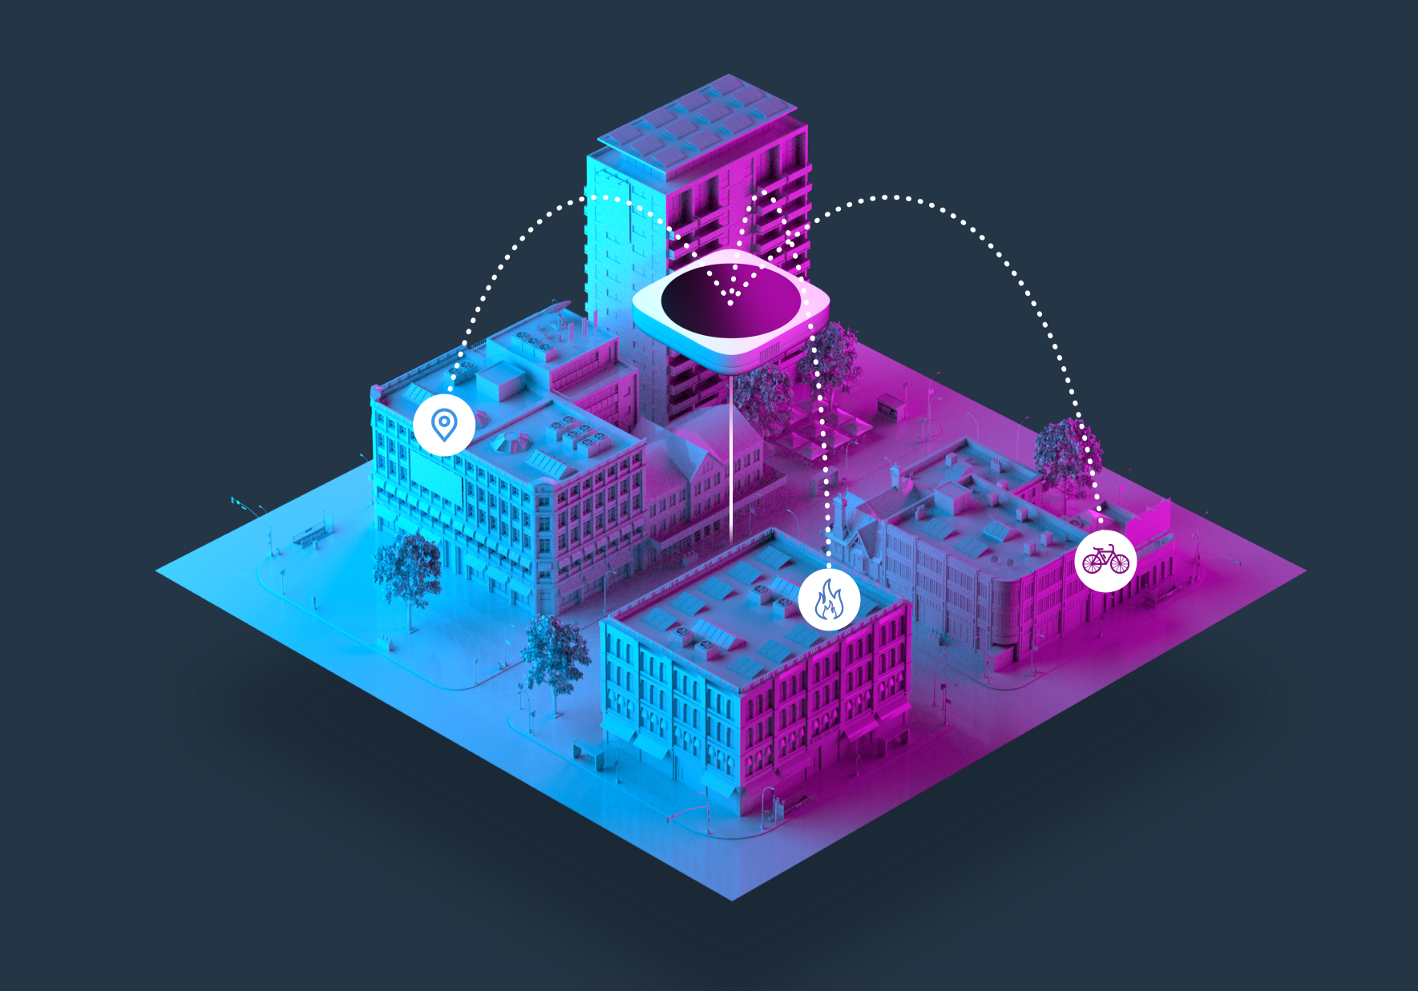
\includegraphics[width=0.9\textwidth]{images/helium.png}
    \caption{Illustration of a helium gateway providing coverage to IoT devices\cite{helium}}
    \label{fig:helium}
\end{figure}

\section{Storage Layer}

Another project that not only influenced the architecture and approach of our solution, but is also included as part of the proposed architecture, is Filecoin. Filecoin wants to turn the world’s unused storage into a decentralized algorithmic market, where anyone can offer his unused storage and be compensated for it, while clients can use the network to store their data. It is built on top of a very successful distributed file system called \acrfull{ipfs}, which is usually referred to as the decentralized HTTP. Although the project is still under heavy development, it is foreseen that the free-market economics of the project will render it a cheaper solution versus the already established storage solutions (such as Google Cloud, AWS, etc.). The Filecoin protocol will be described in depth in Section \ref{st:filecoin}. 


Decentralization offers the elimination of the single point of failure,  a point which is more interesting than it seems, even with the high-availability services that exist today. Recently, a user in twitter \cite{gigazine} mentioned that because of an AWS datacenter power failure (which was coupled with a failure of the on-site backup power generators), the entire datastore of his companies data was erased. Even though the data was restored, because of the timely backup routine, in different scenarios where the data influx is much greater (such as a typical IoT scenario), this power failure could create a hole in the historical data of the platform. Finally, an interesting argument for decentralization is that censorship is impossible to be conducted in a decentralized ecosystem. We must remember that although the Cloud providers have a strong incentive to act in a faithfuly, they are in fact in control of the data we store, a point which depending on the application vertical can have more or less importance, especially in privacy sensitive scenarios (e.g healthcare technology).

Taking into account our need for a storage network, as a means to reduce storage costs, and decentralization there are a couple of projects that we could potentially use, namely: 1)StorJ\cite{storj}, 2)Sia\cite{sia} and 3)Filecoin\cite{filecoinlabs}. We outline some of their attributes and we conclude on why Filecoin was chosen.

\begin{enumerate}
    \item \textbf{Sia:}
    
Sia is an early project that started back in 2013 at HackMIT and officially launched in 2015. It aims to leverage underutilized hard drive capacity around the world to create a data storage marketplace which is more efficient and cheaper to current solutions. They have a working product and have interesting design features. They have preference for the Proof-of-Work(PoW), have their own ASIC chips for Siacoin mining and utilise file contracts to set rules and requirements for storage (similar to a smart contract). Their Proof of Storage algorithm is utilised to further protect and validate proofs and file contracts on the network.

\item \textbf{StorJ:}

Another decentralised storage project, built on the Ethereum network that has quite a lot of community users and is dedicated to the open-source ethos. Storj is a platform, cryptocurrency, and suite of decentralized applications that allows you to store data in a secure and decentralized manner.

Their technology revolves around file sharing, similarly to how torrents work and separates parts of the files to users in the network. When a user wants the file, he requests it and Storj uses a distributed hash table to locate all the shards and piece them together. These files are also encrypted before sharing and the person uploading it has their own private key to validate ownership. The other entity of the company Storj Labs is the for-profit side that rents out it’s network to thousands of users and charges for the network usage. This is a slightly more centralised model and competes with the likes of Dropbox and Google Drive. They also have partnerships with Microsoft Azure and Heroku to deploy some of their development tools which is a great initiative for the open source developer ecosystem.

\item \textbf{Filecoin + IPFS:}

The InterPlanetary File System (IPFS)\cite{ipfslabs} is a protocol started by Protocol Labs to create a new way to server information on the web. Currently the Internet works off a location based addressing where you go to a URL like medium.com which has an IP of X.X.X.X and then you get served your articles. These URL’s are pointed to certain servers around the world. Instead, what IPFS does is serving information based on what it is as opposed to where it is (location). With their routing algorithms, a user can choose where he gets the content from and he can set his privacy on what peers/nodes he trusts to receive the files from. A high level overview of the protocol is shown in Figure \ref{fig:ipfs} \cite{ipfslabs}.

\begin{itemize}
    \item  Hash addressing makes the content immutable. It does not disappear like current HTTP protocol.
    \item Saves bandwidth by collecting content from multiple nodes and pieces instead of from one server.
    \item Access to content “offline” or in low connectivity 3rd world or rural areas, in the same sense that git works offline.
    \item Censorship resistant.
    \item It is built around the decentralisation ethos.

\end{itemize}

To further utilise this technology, Filecoin was proposed as a way of creating a decentralised storage network by using the unused storage lying around and incentivize users to be part of the sharing economy through Filecoins (FIL) by using the IPFS protocol. The project is still under heavy development, so it will be interesting to see how they build with their proposed Proof of Space and Proof of Replication consensus algorithms, which will be discussed further in the Architecture Chapter \ref{ch:system-architecture}. 
\end{enumerate}

\begin{figure}[h]
    \centering
    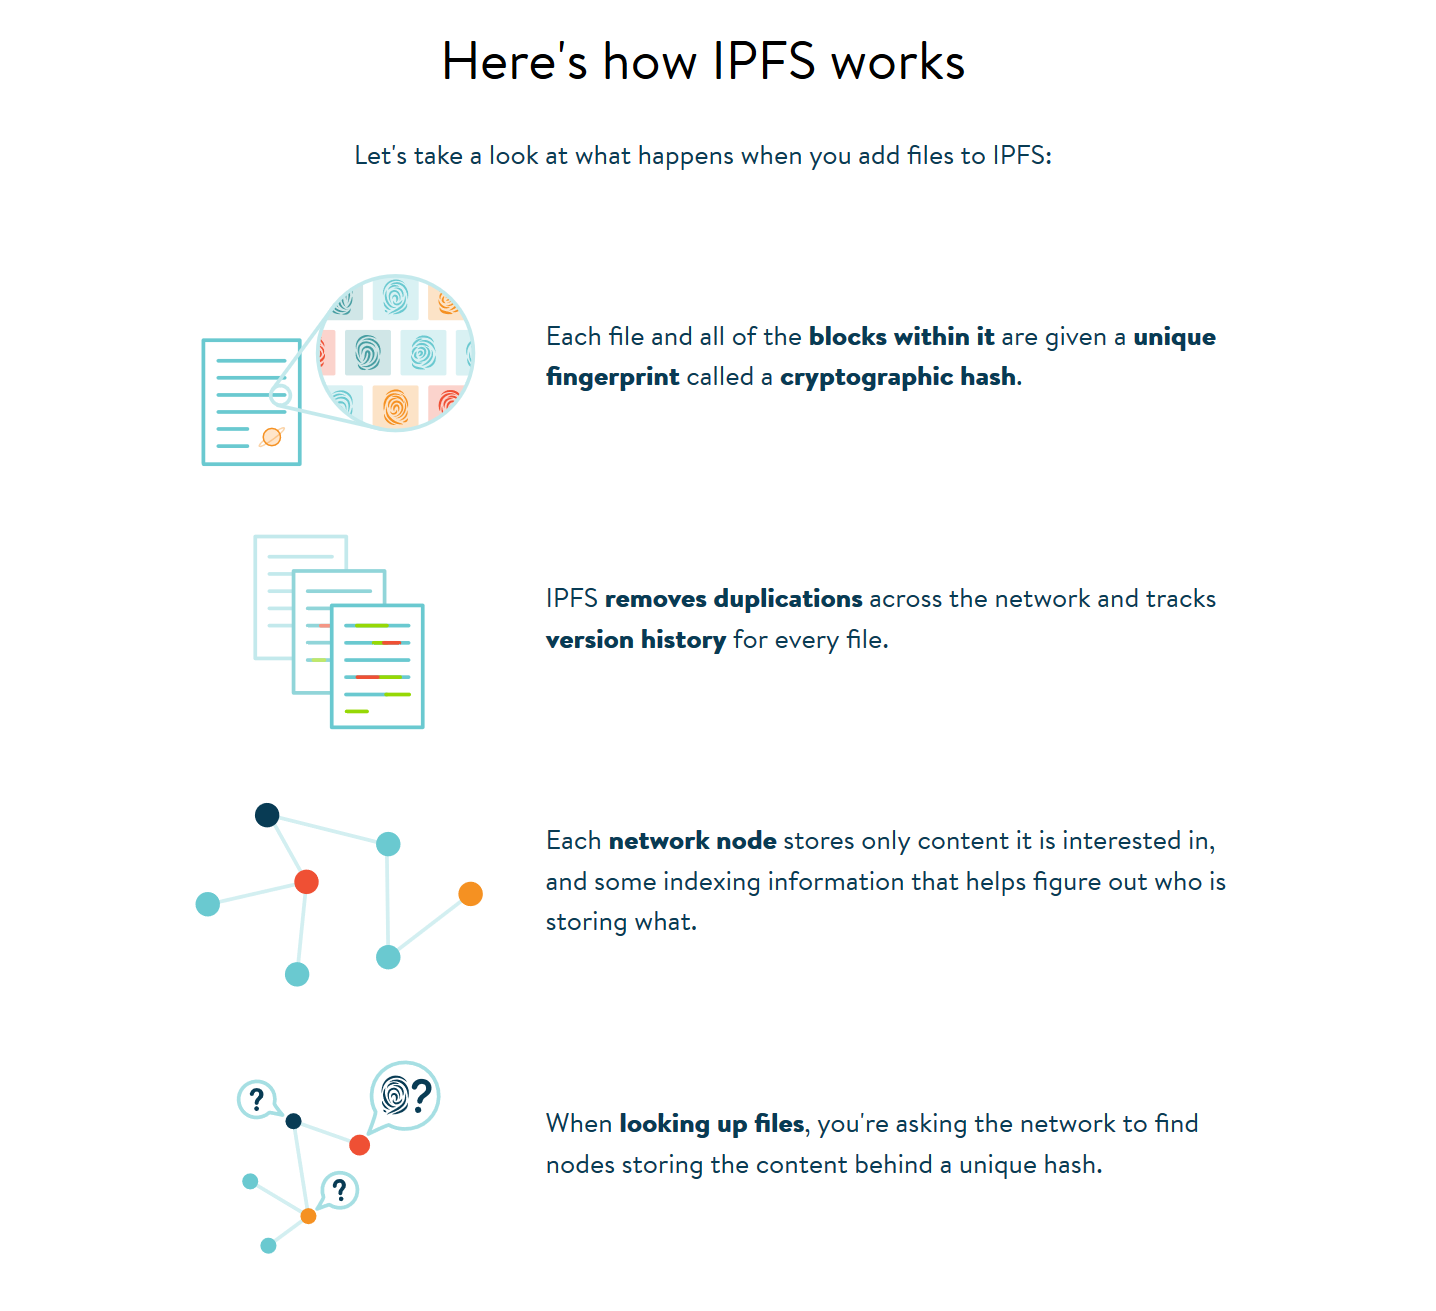
\includegraphics[width=0.9\textwidth]{images/ipfs.png}
    \caption{High-Level overview of the IPFS protocol \cite{ipfslabs}}
    \label{fig:ipfs}
\end{figure}

\subsection{Why Filecoin was chosen}

Filecoin was chosen because it already utilizes a protocol that has been used for several years, establishing itself as the standard for the distributed storage of files in the blockchain community. Moreover, Protocol Labs is a proven development team, having already developed IPFS itself, illustrating serious technical capabilities as also a thorough technical approach. Finally, the development of Filecoin is considerably slower than the other projects, as the team establishes the basic research on top of which the technology will be built. The research based orientation and the technical aspects of the Filecoin whitepaper\cite{filecoin-whitepaper} show great promise and care for the engineering quality of the product, aspects that are highly valued in a domain as pioneering as blockchain. We wanted to integrate in our architecture, a solution that can be viewed for the long-term, supporting in the meantime its development by being early adopters and contributors.

\subsection{Data Integrity}

Data integrity is the overall completeness, accuracy and consistency of data, which means that the data must be collected and stored in an tamper-proof and undeletable fashion. This is extremely important for certain problem domains, such as critical infrastructure. Data Integrity can be achieved by enforcing the Edge systems to digitally sign the sensor data while maintaining an end-to-end cryptography between the sensor and the Edge. Moreover, data integrity dictates that data storage is inherently high-available, meaning that the data storage is equally important as the data collection.

The problem of data integrity has been extensively studied in all traditional computing and communication systems and some preliminary results exist for sensor networks\cite{acharya2008data}. Data integrity became extremely relevant after the trend of storing data on the cloud. While it is easy to check data integrity after completely downloading the data to be checked, downloading large amounts of data just for checking data integrity is a considerable waste of bandwidth. Moreover, remote data integrity validation was firstly introduced using the RSA (Rivest–Shamir–Adleman) based methods and afterwards using a challenge-response model, by Shah et al\cite{shah2007auditing}. In the second model, the user challenges the data storage computer system to respond with a succinct proof which will show that indeed he is storing the data. The simplest of such methods is the division of the data into blocks and the hashing them, but there are other methods with increased efficiency\cite{kumar2011data}.

Blockchain technology is a recent candidate for this issue, as it combines the characteristics of an immutable record with a distributed database. There are currently two mains usages of blockchain to enforce data integrity on the data pipeline. 

\begin{enumerate}
    \item Store data directly on the blockchain, extremely secure but raises a lot of issues regarding scalability and performance. Infeasible for large streams of data.
    \item Package data and store a hash on the blockchain. Thus an immutable succinct record of that data is created. A user needs both the data and the hash to verify the correctness of the data.
\end{enumerate}

\section{Use Cases}

As the thesis attempts to introduce an innovative concept in a new domain, it is pertinent to introduce two (2) use cases that will help the reader to understand the usability of the proposed architecture. The first use-case is the one that was chosen to be the objective of the proof of concept implementation, the fault-tolerance scenario. The second is more generic, illustrating the ad-hoc provision of services.

\subsection{Use Case 1: Fault-Tolerance}

The fault tolerance use case was inspired by a scenario, local to the university of Patras. Near the university, there is a bridge called “Rio-Antirio bridge” or as officially named “Charilaos Trikoupis Bridge”. It is one of the world's longest multi-span cable-stayed bridges and the longest of the fully suspended type, as shown in Figure \ref{fig:riobridge}. A true marvel of engineering, it has 4  pillars over an exceptionally difficult area with numerous challenges, namely the frequent earthquakes, the weak ground and the depth of the gulf. A bridge of this magnitude, houses numerous sensors which aid the bridge operators into verifying the integrity and safety of the bridge, while also acting proactively to any challenge that may rise \cite{rion-antirion-bridge}. It is safe to presume that there is an Edge system that aggregates this data, maybe performs some processing and analytics and then feeds the cloud system that offers the rest of the services to the operators.

\begin{figure}[h]
    \centering
    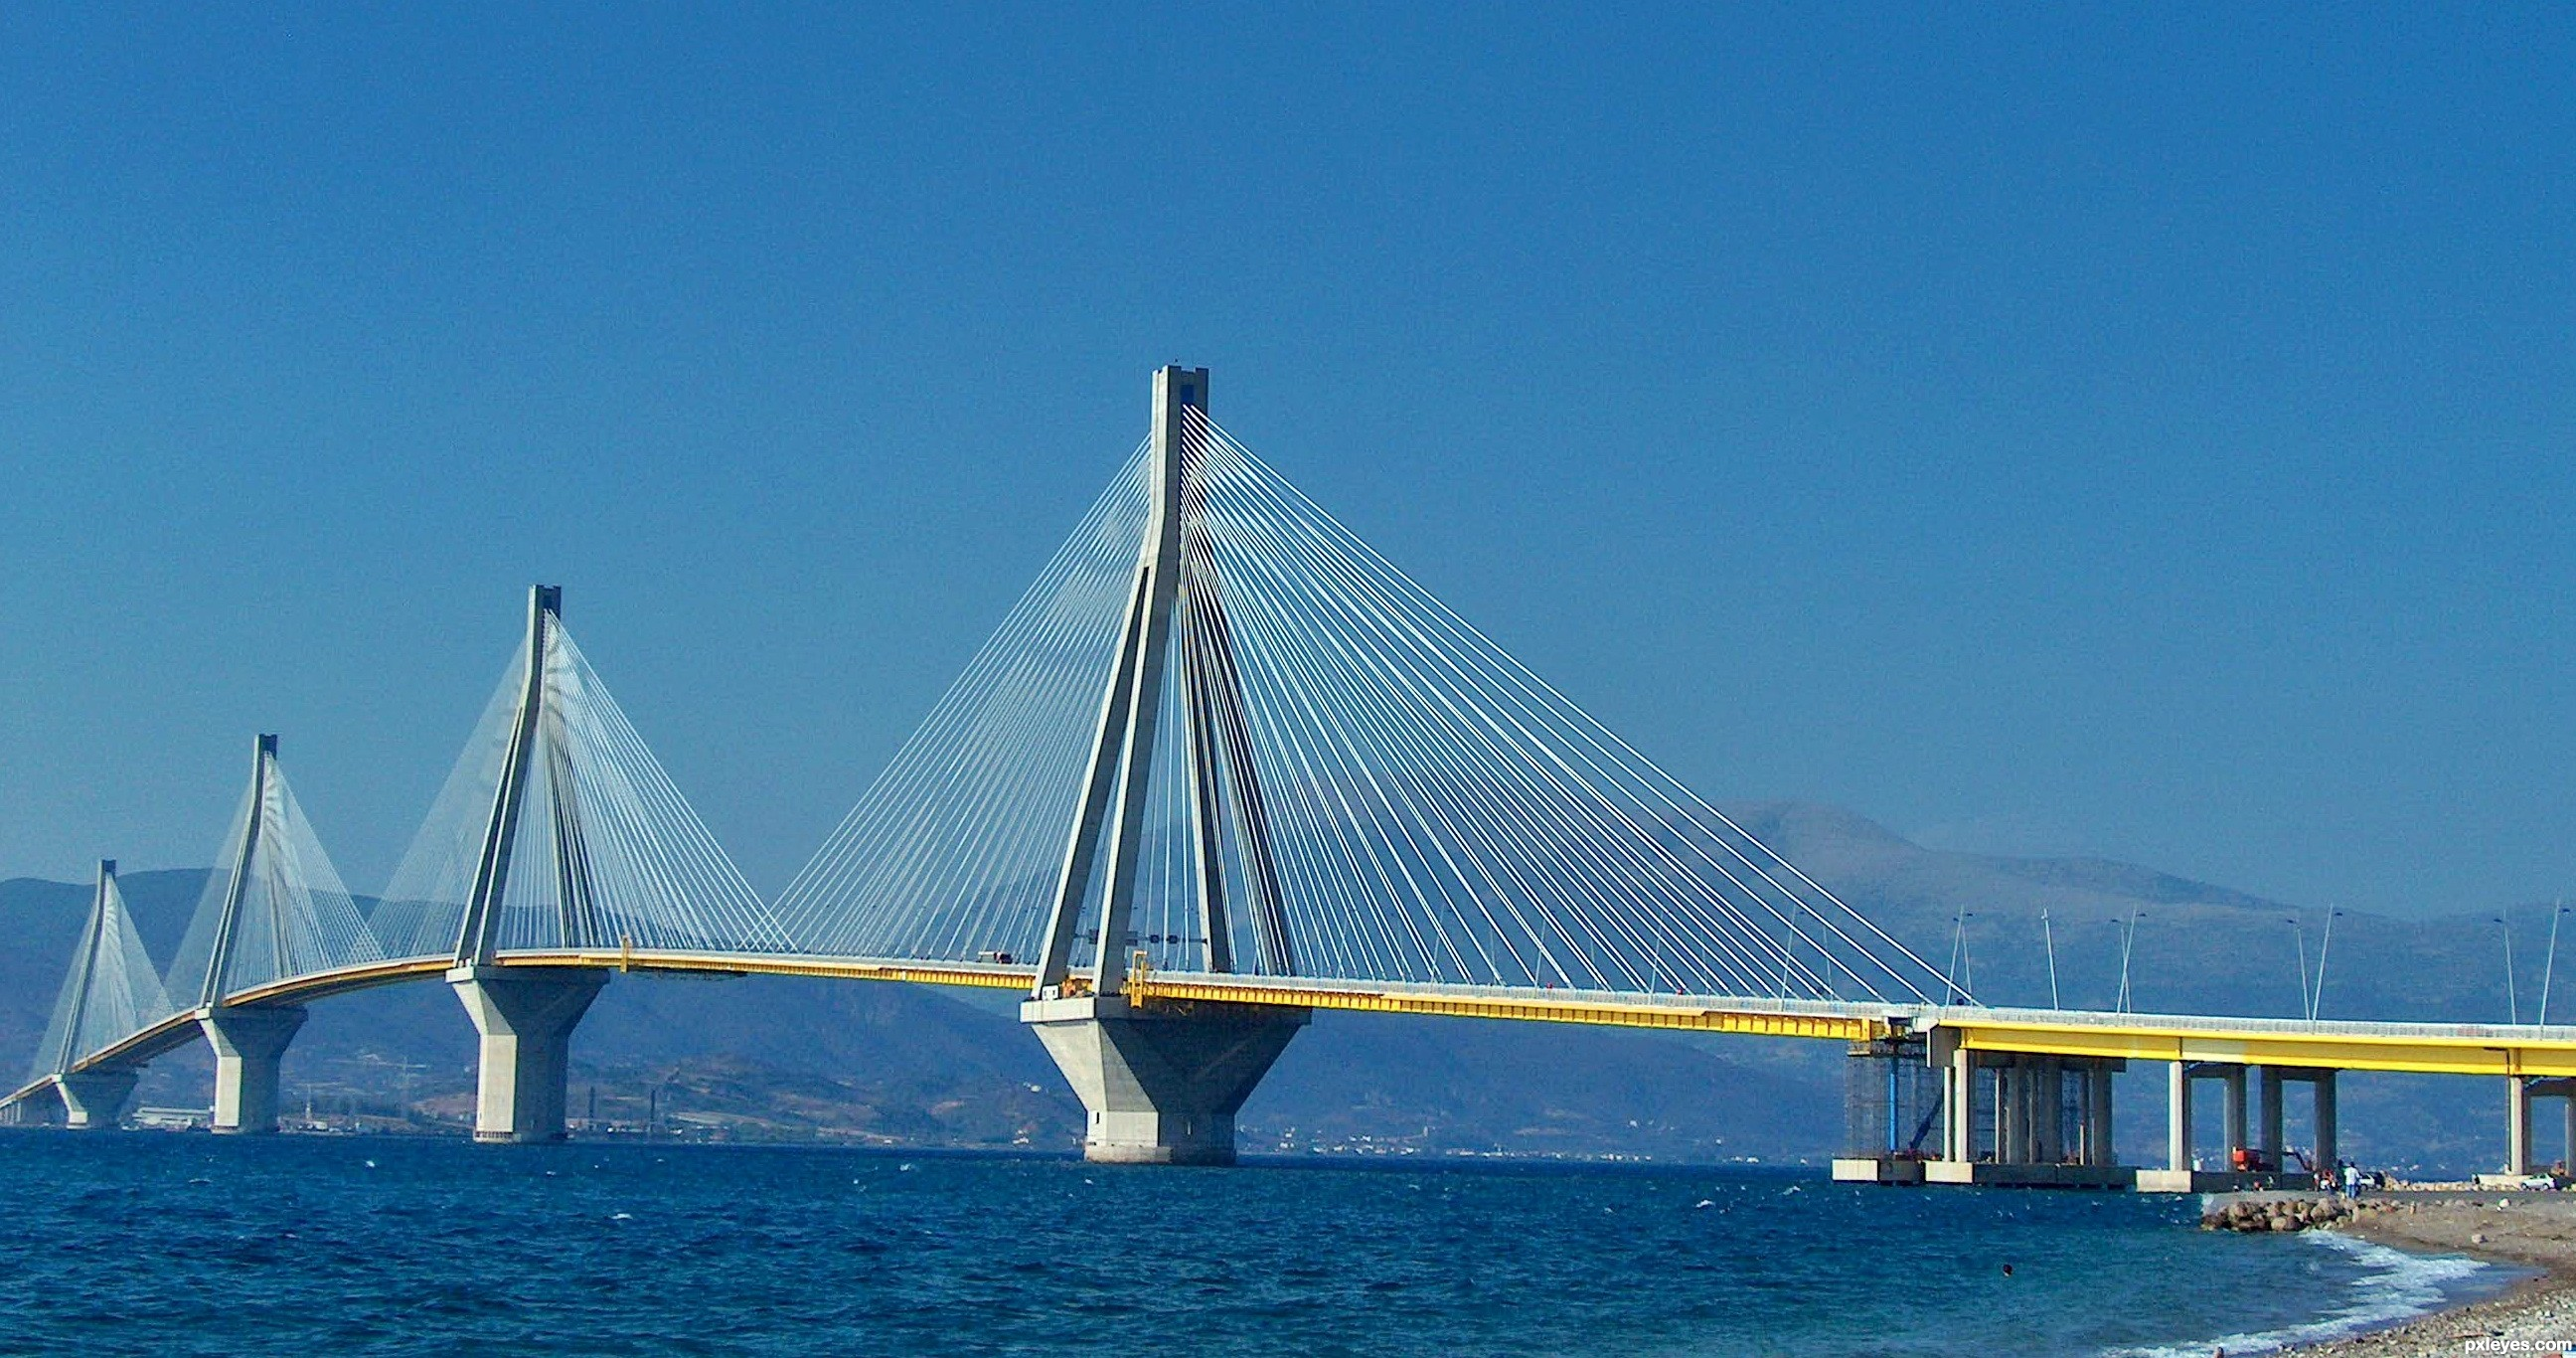
\includegraphics[width=0.6\textwidth]{images/rio-bridge.jpg}
    \caption{The Rio-Antirio Bridge in Western Greece \cite{riowiki}}
    \label{fig:riobridge}
\end{figure}

It is also safe to presume that there are protocols in place for the case that the computer system (“Edge”) fails and the operators are left effectively blind. What would happen if the University of Patras, which is nearby, could in fact jump in with and offer a micro-datacenter, in order to take over the bridge management until the issue is fixed? Due to the extreme locality of the two computer systems, University of Patras can still be considered as “edge” for the Rio-Antirio bridge IoT system. In Figure \ref{fig:rio-map} we see a map overview of the scenario, where the university is clearly indicated by the blue market at the bottom, while the Rio bridge side at the top. The black line that connects the two landmarks is approximately 2.3km, illustrating the extreme locality of the two Edge computers.

\begin{figure}[ht]
    \centering
    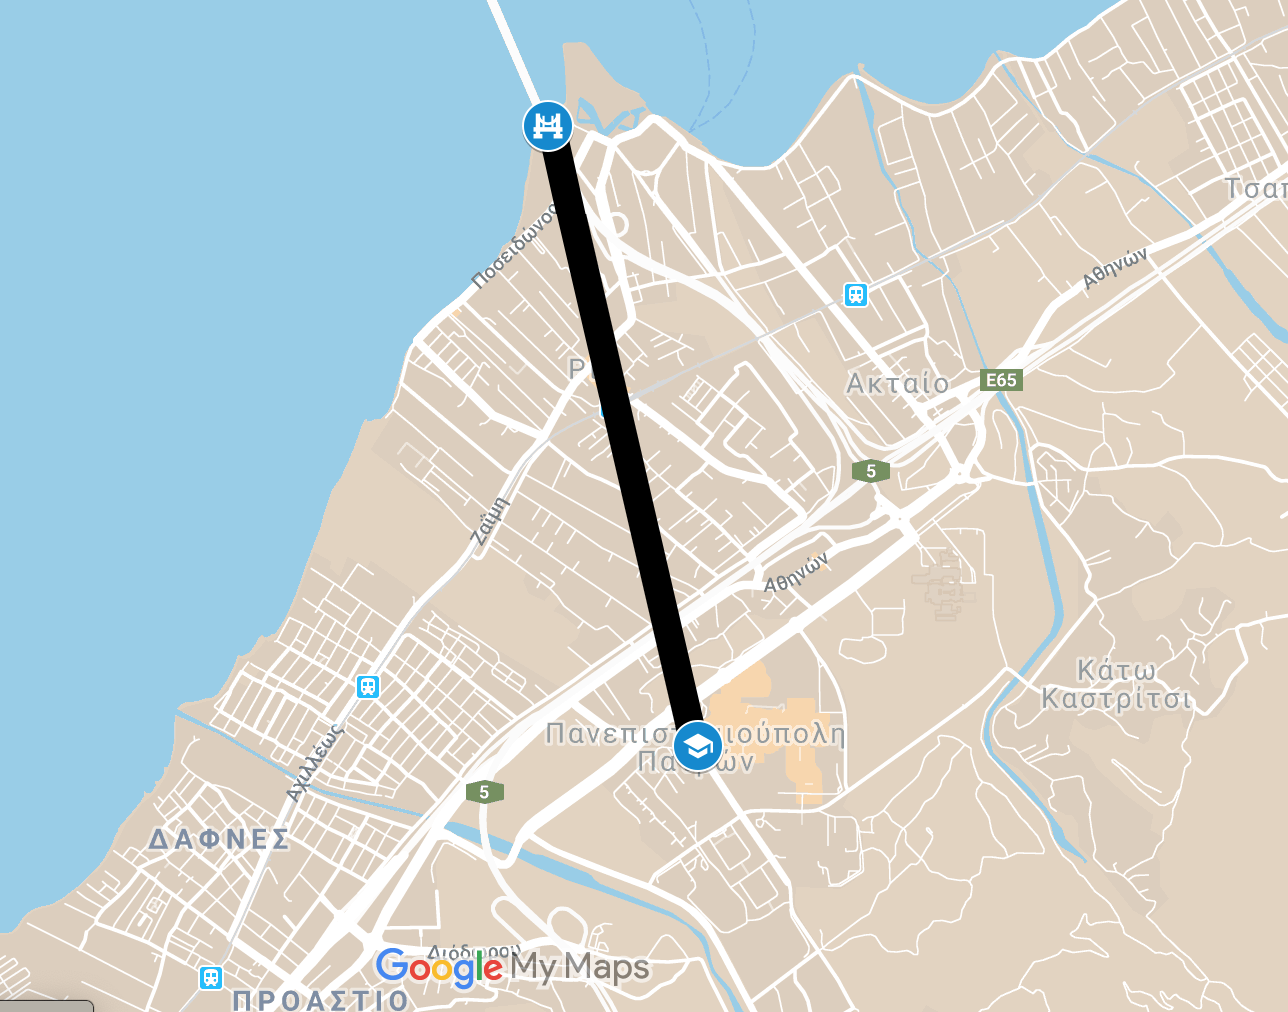
\includegraphics[width=0.6\textwidth]{images/usecase1map.png}
    \caption{A map illustrating the close proximity of the Bridge and the University}
    \label{fig:rio-map}
\end{figure}

The handover of the sensors and all relevant functionality would happen automatically, as soon as a failure was detected by the platform at the University of Patras. The two edge systems would have a priori signed a digital contract, containing all the necessary information, such as needed resources, services, protocols, contract activation conditions and of course payment. The goal is for this dynamic federation to happen in an automated fashion, on a platform that will guarantee the Quality of Service needed for such an important critical infrastructure.

\subsection{Use case 2: Drone passage over IoT Edge Nodes}

The second use-case is more generic in order to showcase the robustness of the architecture over a broad spectrum of issues. In this use-case, we envision a drone that flies over a predetermined route in order to perform some specialized functionality. This drone activity is characterized by three important aspects: 

\begin{enumerate}
    \item  It generates a large number of raw data (such as video feed).
    \item It needs to perform pre-processing before sending it to the cloud due to bandwidth limitations.
    \item Limited battery capacity.
\end{enumerate}

It is apparent that the processing of the data can not be done on the drone itself as the battery would be impossible to realistically handle the consumption demands of the CPU, coupled with the inherent power consumption hungry nature of a drone (i.e the motors). For this reason, the drone knowing the route beforehand, has reached an agreement with a number of edges that are geographically near the route in order to offload the pre-processing and cloud forwarding to them. The drone would then simply fly and stream the data to them, while the IoT Edges will know exactly what to do and what specifications their services need to meet. The streaming could use a low-range protocol such as WiFi or Bluetooth. Figure \ref{fig:drone_map} illustrates an autopilot program for drones \cite{ardupilot}, which enables drone to fly over a predetermined route.

\begin{figure}[h]
    \centering
    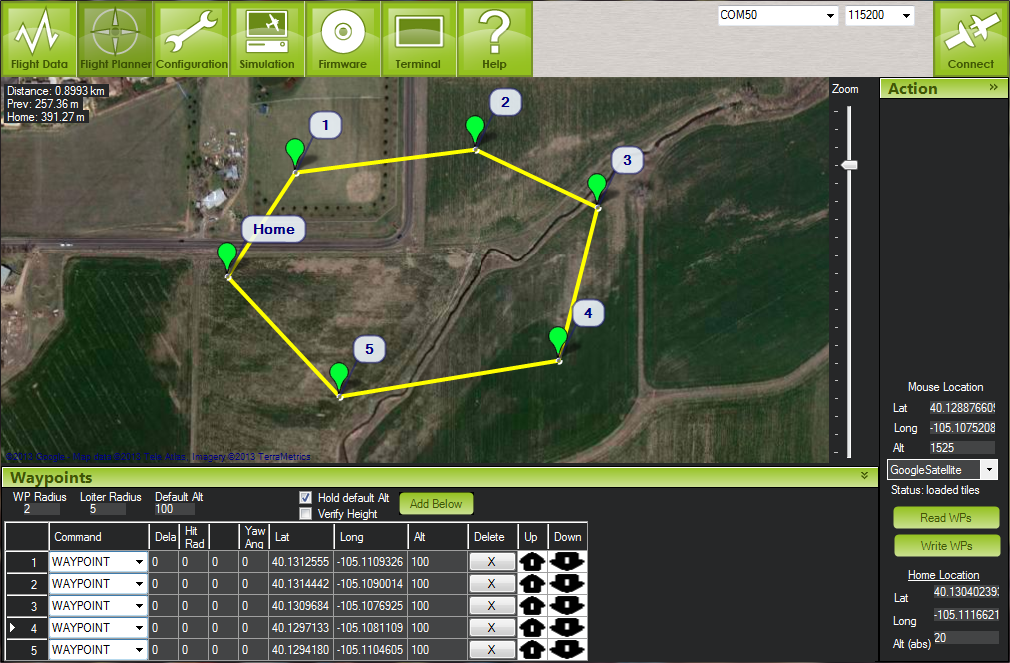
\includegraphics[width=0.7\textwidth]{images/droneroute.png}
    \caption{The GUI of a Drone route mapping software\cite{ardupilot}}
    \label{fig:drone_map}
\end{figure}
 \clearemptydoublepage
 
 \chapter{System Architecture} \label{ch:system-architecture}
\markboth{System Architecture}{}

\paragraph{}
We propose to tackle system redundancy in both the IoT Edge \& Cloud layer by designing an architecture where IoT Edge \& Cloud systems of different stakeholders can dynamically enter into a federation, agreeing that in case of one’s failure (degraded \gls{stakeholder}), the other stakeholder will kick-start a mechanism in order to conduct \gls{iot-management} of the (degraded stakeholder’s) devices. This is a dynamic process, where the systems have access to a centralized marketplace in order to find the optimum option. While our research and implementation focused on the IoT Edge layer, the exact principles can be applied in the cloud layer, although the actual parameters and implementation rest outside of the scope of this work.

In this Chapter we will go through the principles of the proposed architecture and discuss on the core technologies  we choose as the basis of the architecture. We will firstly address the architecture as a whole, starting with the main architectural paradigm, that of micro-services. We then proceed to talk about the technology that enables the provision of resources to run 3rd party services on the same hardware(i.e container technology). Finally, we will delve into the two main subsystems, that is the IoT Edge and the Cloud and their respective modules.

The proposed architecture is intended to serve as a high-level overview of the envisaged components and processes. The specification of each component and core activity, such as the algorithms and state machines, are expected to be presented in a future work. Moreover, we choose to focus on a narrow aspect for the architecture in order to realise our proof of concept, implementing only the core modules of this architecture.

\section{Proposed Architecture}

\begin{figure}[h]
    \centering
    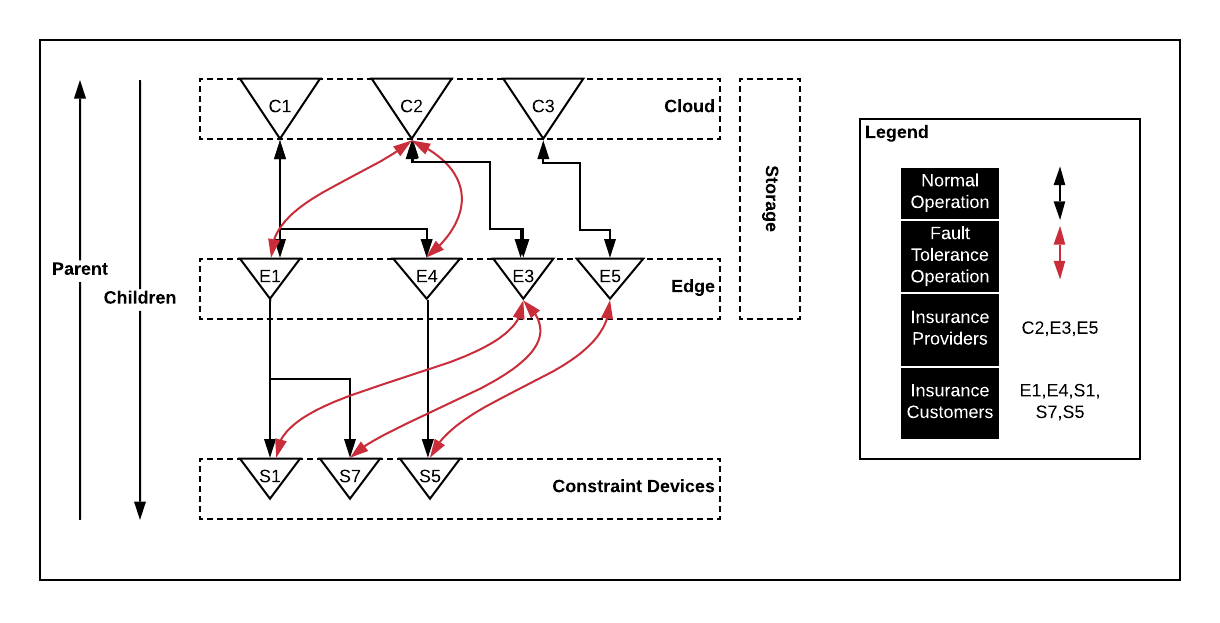
\includegraphics[width=1\textwidth]{images/layer-fault-tolerant.png}
    \caption{The hierarchy layered architecture during normal and fault-tolerance operation}
    \label{fig:hier-fault}
\end{figure}

Figure \ref{fig:hier-fault} outlines the hierarchy and layering of the proposed system design. The normal operation illustrates an \gls{iot-connection} between devices that belong to the same stakeholder (“owner”), while the “Fault-Tolerance” operation illustrates a connection between devices that belong to different stakeholders, and thus there is an exchange of service/value.
 
For each stakeholder’s cloud, his IoT Edge devices are considered his \textbf{children} and the sensors of each IoT Edge system are the \textbf{children} of that particular Edge. 

\begin{figure}[h]
    \centering
    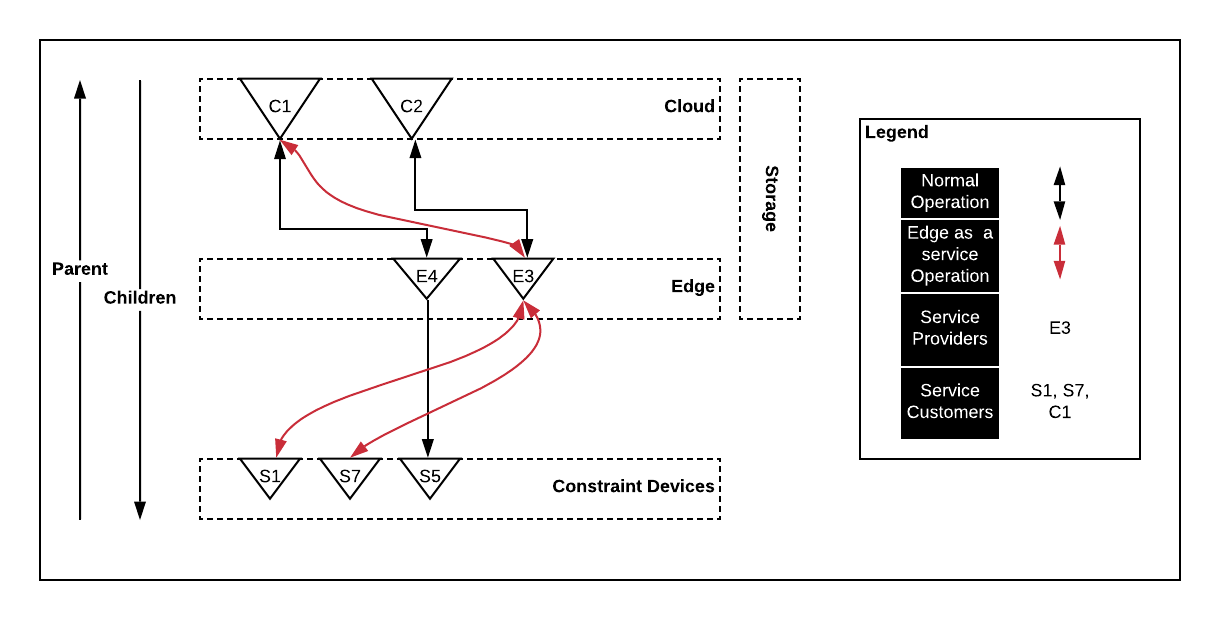
\includegraphics[width=1\textwidth]{images/layer-service-provision.png}
    \caption{The hierarchy layered architecture during "IoT Edge as a service" Operation}
    \label{fig:hier-service}
\end{figure}

Figure \ref{fig:hier-service} shows the same hierarchy but in a more generic scenario, that of the “IoT Edge as a Service” or “EaaS”.  The normal operation illustrates a connection between devices that belong to the same stakeholder (“owner”), while the “IoT Edge as a service” operation illustrates a connection between devices that belong to different stakeholders, and thus there is an exchange of service/value.

The stakeholder owner of cloud system \textit{C1} and sensors \textit{S1,S7} needs an IoT Edge Computing device to manage his sensors \textit{(S1, S7)}, aggregate their data, pre-process them and lastly forward them to the Cloud \textit{(C1)}. Edge \textit{E3} offers such services, while at the same time it offers services to \textit{C2} which belongs to the same stakeholder as \textit{E3}. In other words, \textit{E3} dynamically and while continuing it’s operations, procures resources as requested by \textit{C1}. In this scenario, since we assume that \textit{S1, S7} are managed entirely by another’s stakeholder Edge device, we say that \textit{S1, S7} are the children of \textit{E3} (albeit for a certain period). \gls{iot-management} is a generic term that includes all the relevant IoT activities a parent device must perform to the children, such as provisioning, aggregation, actuating and others.

\section {Decoupling the Storage Layer}

The System is divided in 4 main subsystems layers (Storage, Cloud, Edge, Sensors).  We chose to add an additional layer to that of the IoT reference 3 tier architecture\cite{tranoris}, that of the Storage. By decoupling the storage layer from the cloud layer-which is usually part of-we envision a system where both Cloud \& IoT Edge systems, use the same long-term storage layer, facilitating the high availability functionality we envision. The entire state of the IoT Edge system is foreseen to be stored in the storage layer, both in terms of application logic and sensor data, at specific intervals. Thus, a IoT Edge Node could be easily replicated while maintaining access to important sensor data. 

\textbf{Coupling} is frequently used in software engineering as a metric for the quality of the program in development. It expresses the degree of interdependence between software modules; how closely two modules are connected and how strong their relationship is.  Two loosely coupled (or decoupled) systems can change independently without having any ripple effects one to another. Moreover, they are easily replaceable and the overall quality of the system is increased.

Considering the same stakeholder/owner, a Cloud is the Parent of multiple Edges and an IoT Edge is the Parent of multiple Sensors. The system is agnostic regarding the Storage and Sensor (Constraint Devices)  layers, as long as they follow the specifications established by the relevant hardware and interfaces. 

In our analysis, the system stakeholder can be divided into two groups:
\begin{itemize}
    \item Service-Provider : The owner of the physical IoT Edge device that procures some of it’s resources to run services of 3rd parties. In the use-case implementation, the service-provider  is the Insurance Provider (since the service is a fault-tolerance insurance).
    \item Service-Customer: The stakeholder who requests to the service-provider  to run a number of services on the IoT Edge of the service-provider . In the use-case implementation, the Service Customer is the Insurance Customer (since the service is a fault-tolerance insurance).
\end{itemize}



\section{A design based on Microservices}

Microservices are a software engineering technique, a variant in essence of the Service Oriented Architecture (SOA). It defines that an application is structured as a collection of loosely coupled services\cite{8354433}, which are extremely fine-grained implementing lightweight communication protocols. A service in a SOA usually have 4 main properties \cite{service-oriented-architecture}:
\begin{enumerate}
    \item It logically represents a business activity with a specified outcome.
    \item It is self-contained.
    \item It is a black box for its consumers.
    \item It may consist of other underlying services.
\end{enumerate}

This architecture boosts modularity, since each service can be replaced, updated or change without affecting the overall system. Moreover, since each service is independent, it facilitates the understanding of the system (since each service is viewed as an autonomous micro-system), it boosts development speed as teams can develop services in parallel and facilitates deployment and continuous integration (CI) \cite{microservices.io}.

Microservices usually communicate over a local network using a technology-agnostic protocol, more commonly HTTP. They are independently deployable and more importantly can be developed using different programming technologies, databases and in general heterogenous technologies, as long as the interfaces match in protocols and structure. 

They are commonly found in cloud-native applications using the container technology to facilitate deployment, a method that was followed in our solution. Finally, it is worth noting that a microservice cannot be part of a monolithic application. Rather it is a self-contained piece of business functionality with clear interfaces, and may, through its own internal components, implement a layered architecture. From a strategy perspective, microservices architecture follows the Unix philosophy of "Do one thing and do it well"\cite{krause2015microservices}.

\subsection{Why Microservices}

The microservices paradigm was chosen for 2 main reasons:
\begin{enumerate}
    \item Our goal is to create a platform where an agent (i.e user, device)  can rent resources to run services on a 3rd party IoT Edge device. Having a microservices architecture, it is extremely easy to implement a platform where services can be added and remove on an ad-hoc basis, without affecting the overall functionality of the system.
    \item The system was built around the EdgeX Foundry Internet of Things platform. EdgeX foundry architecture is that of microservices, so it was easier to integrate our custom modules to an already established IoT platform, which we will describe in the following Subsection \ref{sub:edgex}.
\end{enumerate}

\subsection{EdgeX Foundry} \label{sub:edgex}

EdgeX Foundry\cite{edgex-foundry} is a vendor-neutral open source project, under the auspices of the Linux foundation. It builds a common open framework for IoT Edge Computing in the domain of Internet of Things. At the core of the initiative,lies an interoperability framework hosted within a full hardware and OS agnostic reference software platform. It enables an ecosystem of plug-and-play components that unifies the existing IoT Edge marketplace and accelerates the development and deployment of Internet of Things solutions.

The project was spearheaded by Dell in 2017 and later open sourced under Linux Foundation. Several companies (such as Dell, Redis, and others) are actively contributing to the project which also has a vibrant community. 

\begin{figure}[h]
    \centering
    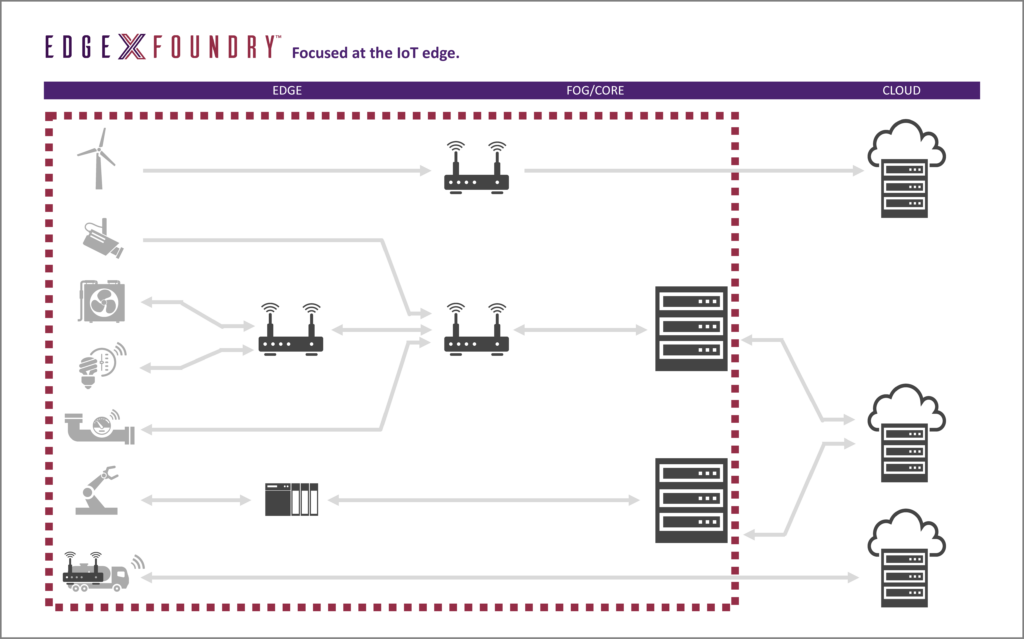
\includegraphics[width=0.6\textwidth]{images/edgex_arch1.png}
    \caption{The project focus of EdgeX Foundry in the IoT stack}
    \label{fig:edgex_focus}
\end{figure}

EdgeX foundry focuses on the Industrial IoT Edge, shown in Figure \ref{fig:edgex_focus} leveraging cloud-native principles, such as loosely-coupled microservices and platform independence, to architect around the needs of the IoT Edge. It mainly targets IoT Edge Nodes such as gateways, routers and embedded PCs and their interoperability. It can run on a single IoT Edge or be distributed over a larger number.

\begin{figure}[h]
    \centering
    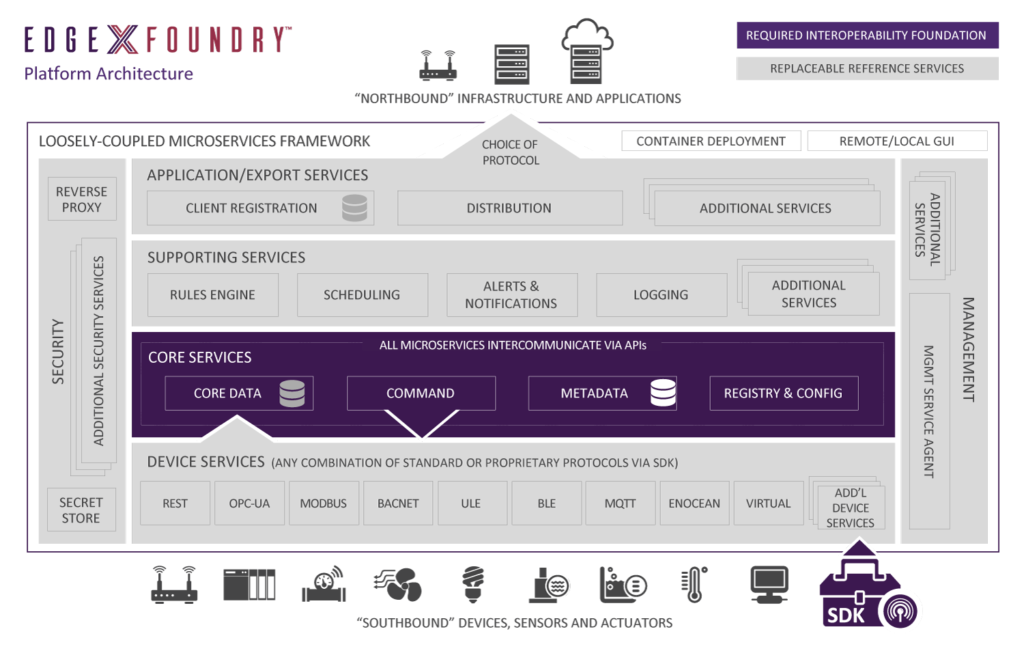
\includegraphics[width=0.9\textwidth]{images/edgex_arch.png}
    \caption{The EdgeX high-level architecture}
    \label{fig:edgex_arch}
\end{figure}

Figure \ref{fig:edgex_arch} illustrates the EdgeX platform architecture, each square indicates a different microservice, which are grouped based on their functionality in the platform. A user can select to run only a subset of the available microservices, except for the core services (Purple) which are needed as a whole. The device service SDK\cite{device-service-sdk} is needed to interface any Constrained Device to the platform.

The grey microservices are reference services that constitute a fully functional IoT Edge software, but they are optional. EdgeX is fully agnostic concerning the \gls{north-side} and \gls{south-side} of the platform, as such we can even create a layered architecture of multiple EdgeX that perform different functionalities, as shown in Figure \ref{fig:edgex_fog_layer}.

EdgeX foundry is currently under heavy development and the reference implementation is in Go. The microservices communicate using HTTP and each has its own \acrfull{rest} interface resource. The suggested deployment method is using Docker Containers, as further discussed in Implementation Chapter \ref{ch:implementation}.

\begin{figure}[h]
    \centering
    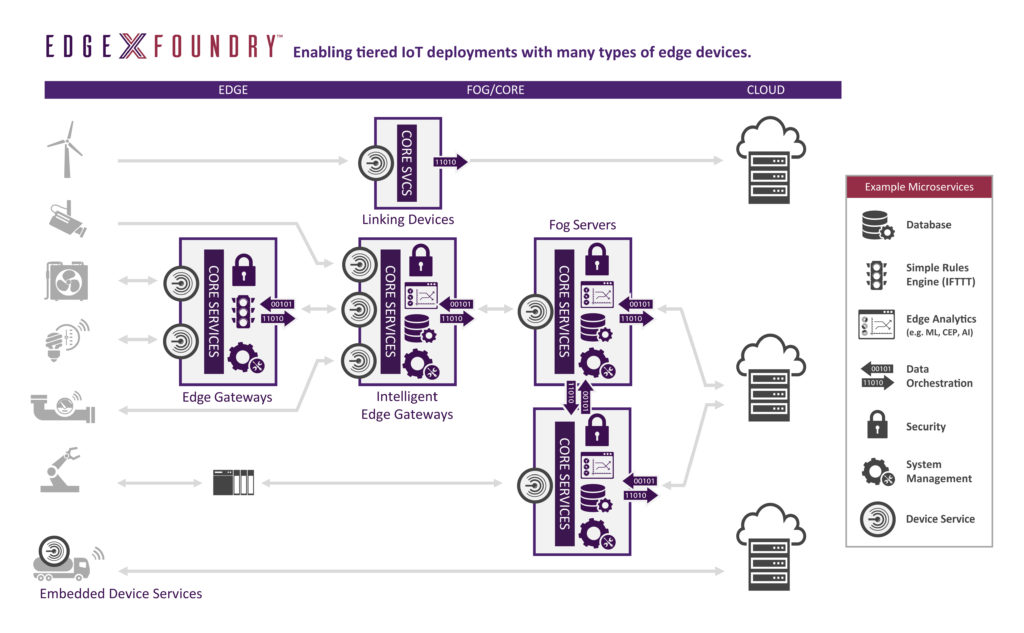
\includegraphics[width=0.9\textwidth]{images/edgex_fog_layer.jpg}
    \caption{A layered approach of fog computing using EdgeX}
    \label{fig:edgex_fog_layer}
\end{figure}

Below we give an apt description of each microservice so the reader better understand our implementation choices, where we choose to deploy only a subset of the available EdgeX foundry microservices.
 
\textbf{Core Services (CS)}
They separate the north and south side layers at the edge. Core services include the following components:
\begin{itemize}
    \item Core data: a persistence repository and associated management service for data collected from the south side objects.
    \item Command: a service that facilitates and controls actuation requests from the north side to the south side.
    \item Metadata: a repository and associated management service of metadata about the objects that are connected to EdgeX Foundry. It provides the capability to provision new devices and pair them with their owning device services.
    \item Registry and Configuration: provides other EdgeX Foundry microservices with information about associated services within EdgeX Foundry and microservices configuration properties. 
\end{itemize}

\textbf{Supporting Services (SS)}
The Supporting Services (SS) Layer encompass a wide range of microservices that provide the IoT Edge analytics and intelligence, and provide service to EdgeX Foundry itself. Normal software application duties such as logging, scheduling, and data clean up (scrubbing) are performed by microservices in the SS Layer. The rules engines, alerting and notification microservices are within the SS Layer because they operate on top of the Core Services Layer. 

EdgeX Foundry operates independently of other systems when necessary. It is able to operate and sustain itself over long periods of time without connection to the “north side” systems. The data and intelligence that is created at the edge, should be collected and transported to enterprise (cloud) systems. The transporting is performed by the Export Services (ES) Layer.

\textbf{Export Services (ES) Layer}
The ES Layer provides a set of microservices that performs the following activities:
\begin{itemize}
    \item Enables off-gateway clients to register for data that interests them, coming from the south side objects.
    \item Informs where and when the data is to be delivered.
    \item Informs the format and shape in which that data is to be delivered.
\end{itemize}

\textbf{Security Elements:}
Security elements both inside and outside of the EdgeX Foundry protect the data and command of devices, sensors, and other IoT objects managed by EdgeX Foundry. The major EdgeX security components are two, the first is a security store that is used to safe place the EdgeX secrets (tokens, passwords, etc.) and the second is an \acrfull{api} gateway that is used as a reverse proxy to restrict access to EdgeX REST resources while also performing access control.

\textbf{System Management:}
The system management facilities provide the central point of contact for external management systems to start or stop EdgeX services and get metrics on the EdgeX services (e.g memory usage).

\section{Containers} \label{st:containers}

Containers are currently finding extensive usage in Cloud platforms as they are one of the 2 main methods to host Platforms as a Service (Paas), the other being the common \acrfull{os} virtualization. Container technology was introduced in 1979\cite{ismail2015evaluation}, when UNIX introduced the Chroot command. Later, in 1988, FreeBSD pioneered with jail that extended Chroot and Sun Solaris introduced Zones, further extending Chroot.In 2001, Linux VServer took from the above jail system and enhanced it by securely partitioning resources on any computer system.

\subsection{Container-based vs traditional virtualization}

\textbf{Containers} are an abstraction at the application layer that packages code and dependencies together. Multiple containers can run on the same machine and share the OS kernel with other containers, each one running as an isolated processes in user space. Containers take up less space than VMs (container images are typically tens of MBs in size).

\noindent
\textbf{Virtual machines} \acrshort{vm} are an abstraction of physical hardware turning one server into many servers. The hypervisor allows multiple VMs to run on a single machine. Each VM includes a full copy of an operating system, the application, necessary binaries and libraries - taking up tens of GBs. VMs can also be slow to boot.

\begin{figure}[h]
    \centering
    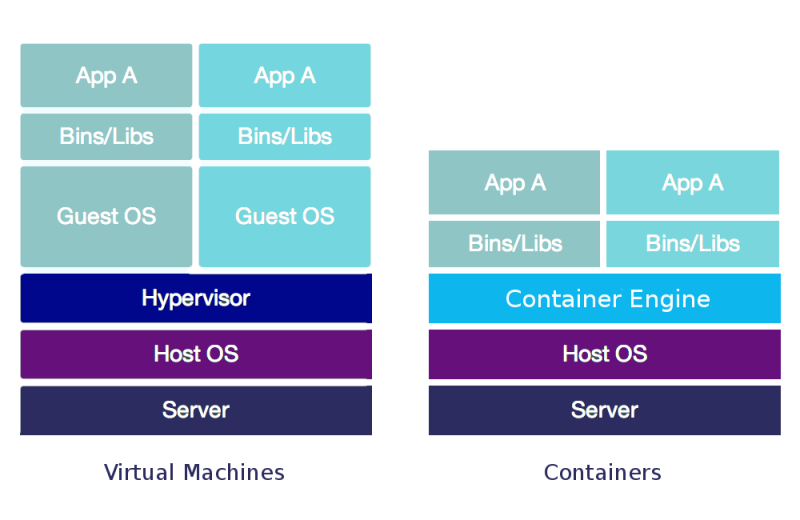
\includegraphics[width=0.6\textwidth]{images/docker_arch.png}
    \caption{Overview of a VM-based and container-based isolation architecture \cite{kumina}}
    \label{fig:container}
\end{figure}

Figure \ref{fig:container} shows the difference in computational overhead regarding traditional virtualization and container-based virtualization. The lightweight approach of containers enable the Host OS to support hundreds of containers on the same hardware.

Thus, containers can be viewed as a standard unit of software, a package which incorporates all the code and dependencies in a unit that can run on any computing system, in a quick and reliable manner.

\subsection{Docker}
Container images become containers at runtime and in the case of Docker containers - images become containers when they run on Docker Engine. Available for both Linux and Windows-based applications, containerized software will always run the same, regardless of the infrastructure. Docker container technology\cite{docker} was launched in 2013 as an open source container Engine. It leveraged existing computing concepts around containers and specifically in the Linux world, primitives known as cgroups and namespaces. The success in the Linux world drove a partnership with Microsoft that brought Docker containers and its functionality to Windows Server.

\subsection{Containers or Images, a clarification}
A container is launched by running an image. An image is an executable package that includes everything needed to run an application--the code, a runtime, libraries, environment variables, and configuration files. A container is a runtime instance of an image--what the image becomes in memory when executed (that is, an image with state, or a user process).

Images are built by the docker engine based on instructions that are written in a Dockerfile \cite{dockerfile} which defines what goes on in the environment inside the container. Access to resources like networking interfaces and disk drives is virtualized inside this environment, which is isolated from the rest of the system. For instance the user might need to instruct Docker to map certain ports from the container to the network interface of the host OS, or copy certain files from the host OS to the container (e.g configuration files, scripts, etc. ), an example is shown in Figure \ref{fig:dockerfile}.
\bigbreak
\noindent
\begin{figure}
\begin{minted}[%
 breaklines,
 mathescape,
 linenos,
 numbersep=5pt,
 frame=single,
 numbersep=5pt,
 xleftmargin=0pt
 ]{dockerfile}
    
# Use an official Python runtime as a parent image
FROM python:2.7-slim

# Set the working directory to /app
WORKDIR /app

# Copy the current directory contents into the container at /app
COPY . /app

# Install any needed packages specified in requirements.txt
RUN pip install --trusted-host pypi.python.org -r requirements.txt

# Make port 80 available to the world outside this container
EXPOSE 80

# Define environment variable
ENV NAME World

# Run app.py when the container launches
CMD ["python", "app.py"]
\end{minted}
\caption{A Dockerfile file example \cite{dockerfile}}
\label{fig:dockerfile}
\end{figure}

\subsection{docker-compose}
Docker compose (also called docker-compose)\cite{docker-compose} is a tool for designing and running multi-container applications. Following Docker‘s one application per container it is difficult to create or to containerize applications that have multiple components or servers. Thanks to docker-compose, the user can easily define multiple services (in a YAML file), link them together and run them. In the YAML file, the user defines each service as also the interdependence of the services. It informs docker on important attributes of each service, such as whether to use a container image from a registry or to build it locally with a Dockerfile. 

It also informs the docker engine on whether there are ports that are needed to be exposed (which can also be defined in a Dockerfile) as also on whether certain containers mush share file systems (using the volumes parameter) or if a service must wait for another before it starts. An example of a docker compose file can be seen in Figure \ref{fig:docker-compose} and further examination of the syntax can be found in the official documents\cite{docker-compose} of docker-compose.
\bigbreak
\begin{figure}[H]
\begin{minted}[%
 breaklines,
 mathescape,
 linenos,
 numbersep=5pt,
 frame=single,
 numbersep=5pt,
 xleftmargin=0pt
 ]{yaml}
version: '3'
services:
  web:
    build: .
    ports:
    - "5000:5000"
    volumes:
    - .:/code
    - logvolume01:/var/log
    links:
    - redis
  redis:
    image: redis
volumes:
  logvolume01: {}

\end{minted}
\caption{A docker-compose.yaml file example \cite{docker-compose}}
\label{fig:docker-compose}
\end{figure}

In conclusion, the Dockerfile defines a single microservice and it’s container, while the docker-compose defines the whole application and the relationships between the containers. There are container attributes that can be set from either file, the choice rests on various parameters of the application deployment.

Finally, Docker started an open-source project, Moby\cite{moby} to enable and accelerate software containerization. It provides a number of toolkit components and a framework for assembling them into custom container-based systems. Quite interestingly, our architecture is based on a project that is in turn based on Moby.


\subsection{Why Containers}

We opted to base our architecture on the containerization of microservices as it is in fact the foundation that makes our concept possible. Since containers are OS and hardware agnostic, the containerized microservices can run natively on any hardware, as long as it has the same CPU architecture (e.g RISC, x86, etc.) .
 
Thus, a service customer \textbf{SC} wishing to run some application logic on the service-provider’s \textbf{SP} Edge, simply: 1) packages the application into a number of clearly defined, stateless microservices, 2) agrees with the service-provider on the resources that \textbf{SP} will make available to the services and then 3) \textbf{SC} sends the container binaries to the \textbf{SP}.
 
It is important to note that the above mentioned 3-step functionality is complex and has many aspects that demand attention, from container management to security. \textit{The notion though rests unchanged.} 

\subsubsection{Container Security}

Security is an aspect that merits attentions, since containers are developed for use in trusted systems and not in multi-tenant environments as in the case of VMs. Containers offer a much more wide attack surface because the containers share the kernel linux. As such, critical bugs could result in malicious code being injected from one container to another or from one container to the hostOS ans vice-versa. Moreover, taken into account the network component of a multi-tenant container setup, containers or the hostOS could act as sniffers of the traffic passing through the same network bridge or even perform Man-in-the-Middle attacks. These kind of attacks can be mitigated by the use of a supervisor service which will monitor the activity of each container or by isolating the containers through multiple network bridges, but a thorough analysis is in order to verify feasibility.

Finally, we remind the user that all containers would run on the same hardware, giving extreme low-level attack surfaces to the IoT Edge owner since he will have physical access to the device.

\subsection{Balena}

For the system and fleet management of our IoT Edge Platform, we opted to choose balena\cite{balena}, a platform that is developed by balena.io, a Greek startup company that was founded in 2014, aiming to bring the docker container technology on IoT Edge devices, a non trivial task as docker container was developed with the needs of cloud computers at mind and not the unique needs and attributes of the relatively constrained IoT Edge devices (e.g Raspberry pi, Beaglebone, Intel Edison, etc.).

Balena offers a complete set of tools to manage and deploy fleets of connected Linux devices, i.e IoT Edge devices. Balena has many features, that we will mention in this subsection, but it’s pertinent to start with the one that interests us the most.

Balena has developed a bare-bones Yocto Linux based OS, named BalenaOS\cite{balenaos}, that can run on many common IoT Edge devices and architectures (e.g aarch64, armv7, etc.). In essence, to deploy applications on a balena powered device, the user deploys containers and manages them through the balena supervisor and balenaCloud\cite{balenacloud}. On top of that, balena has developed its own lightweight container technology, called balenaEngine\cite{balenaengine}, that is based on the Moby project and offers a docker compatible container technology that is \textit{superbly} optimised for the Edge.

\begin{figure}[h]
    \centering
    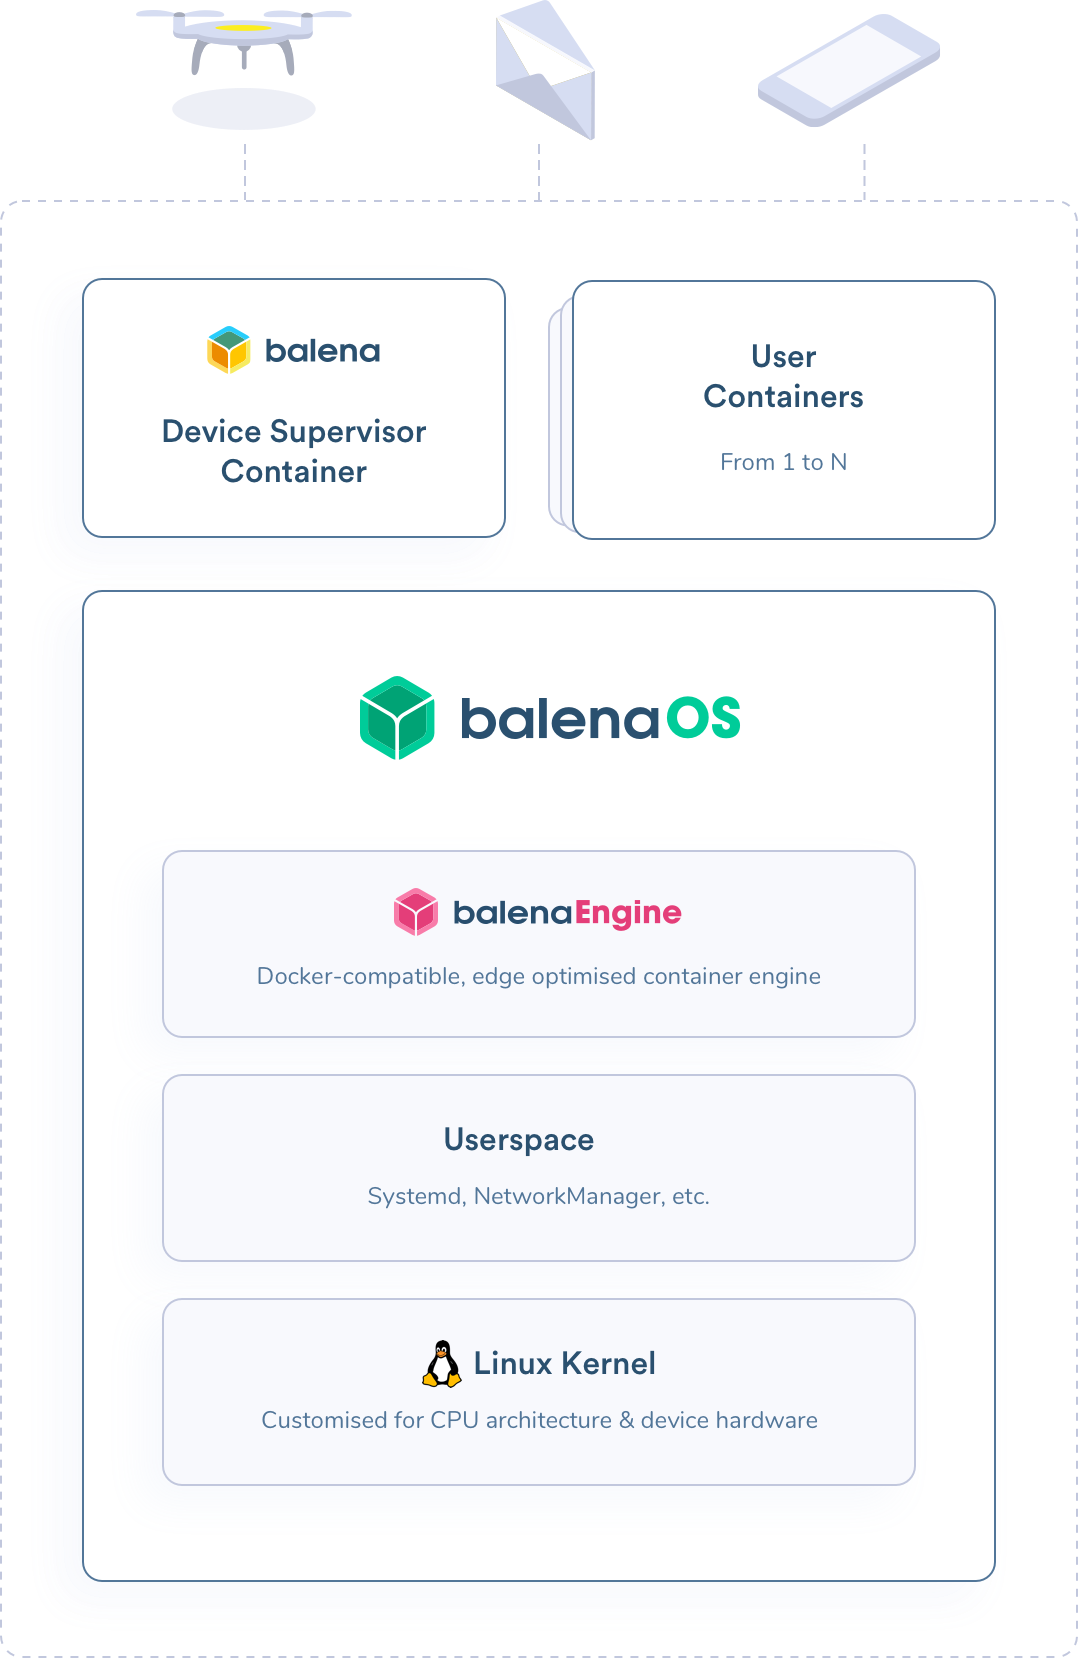
\includegraphics[width=0.5\textwidth]{images/balena_arch.png}
    \caption{The BalenaOS architecture \cite{balenaos}}
    \label{fig:balena_arch}
\end{figure}

\begin{figure}[h]
    \centering
    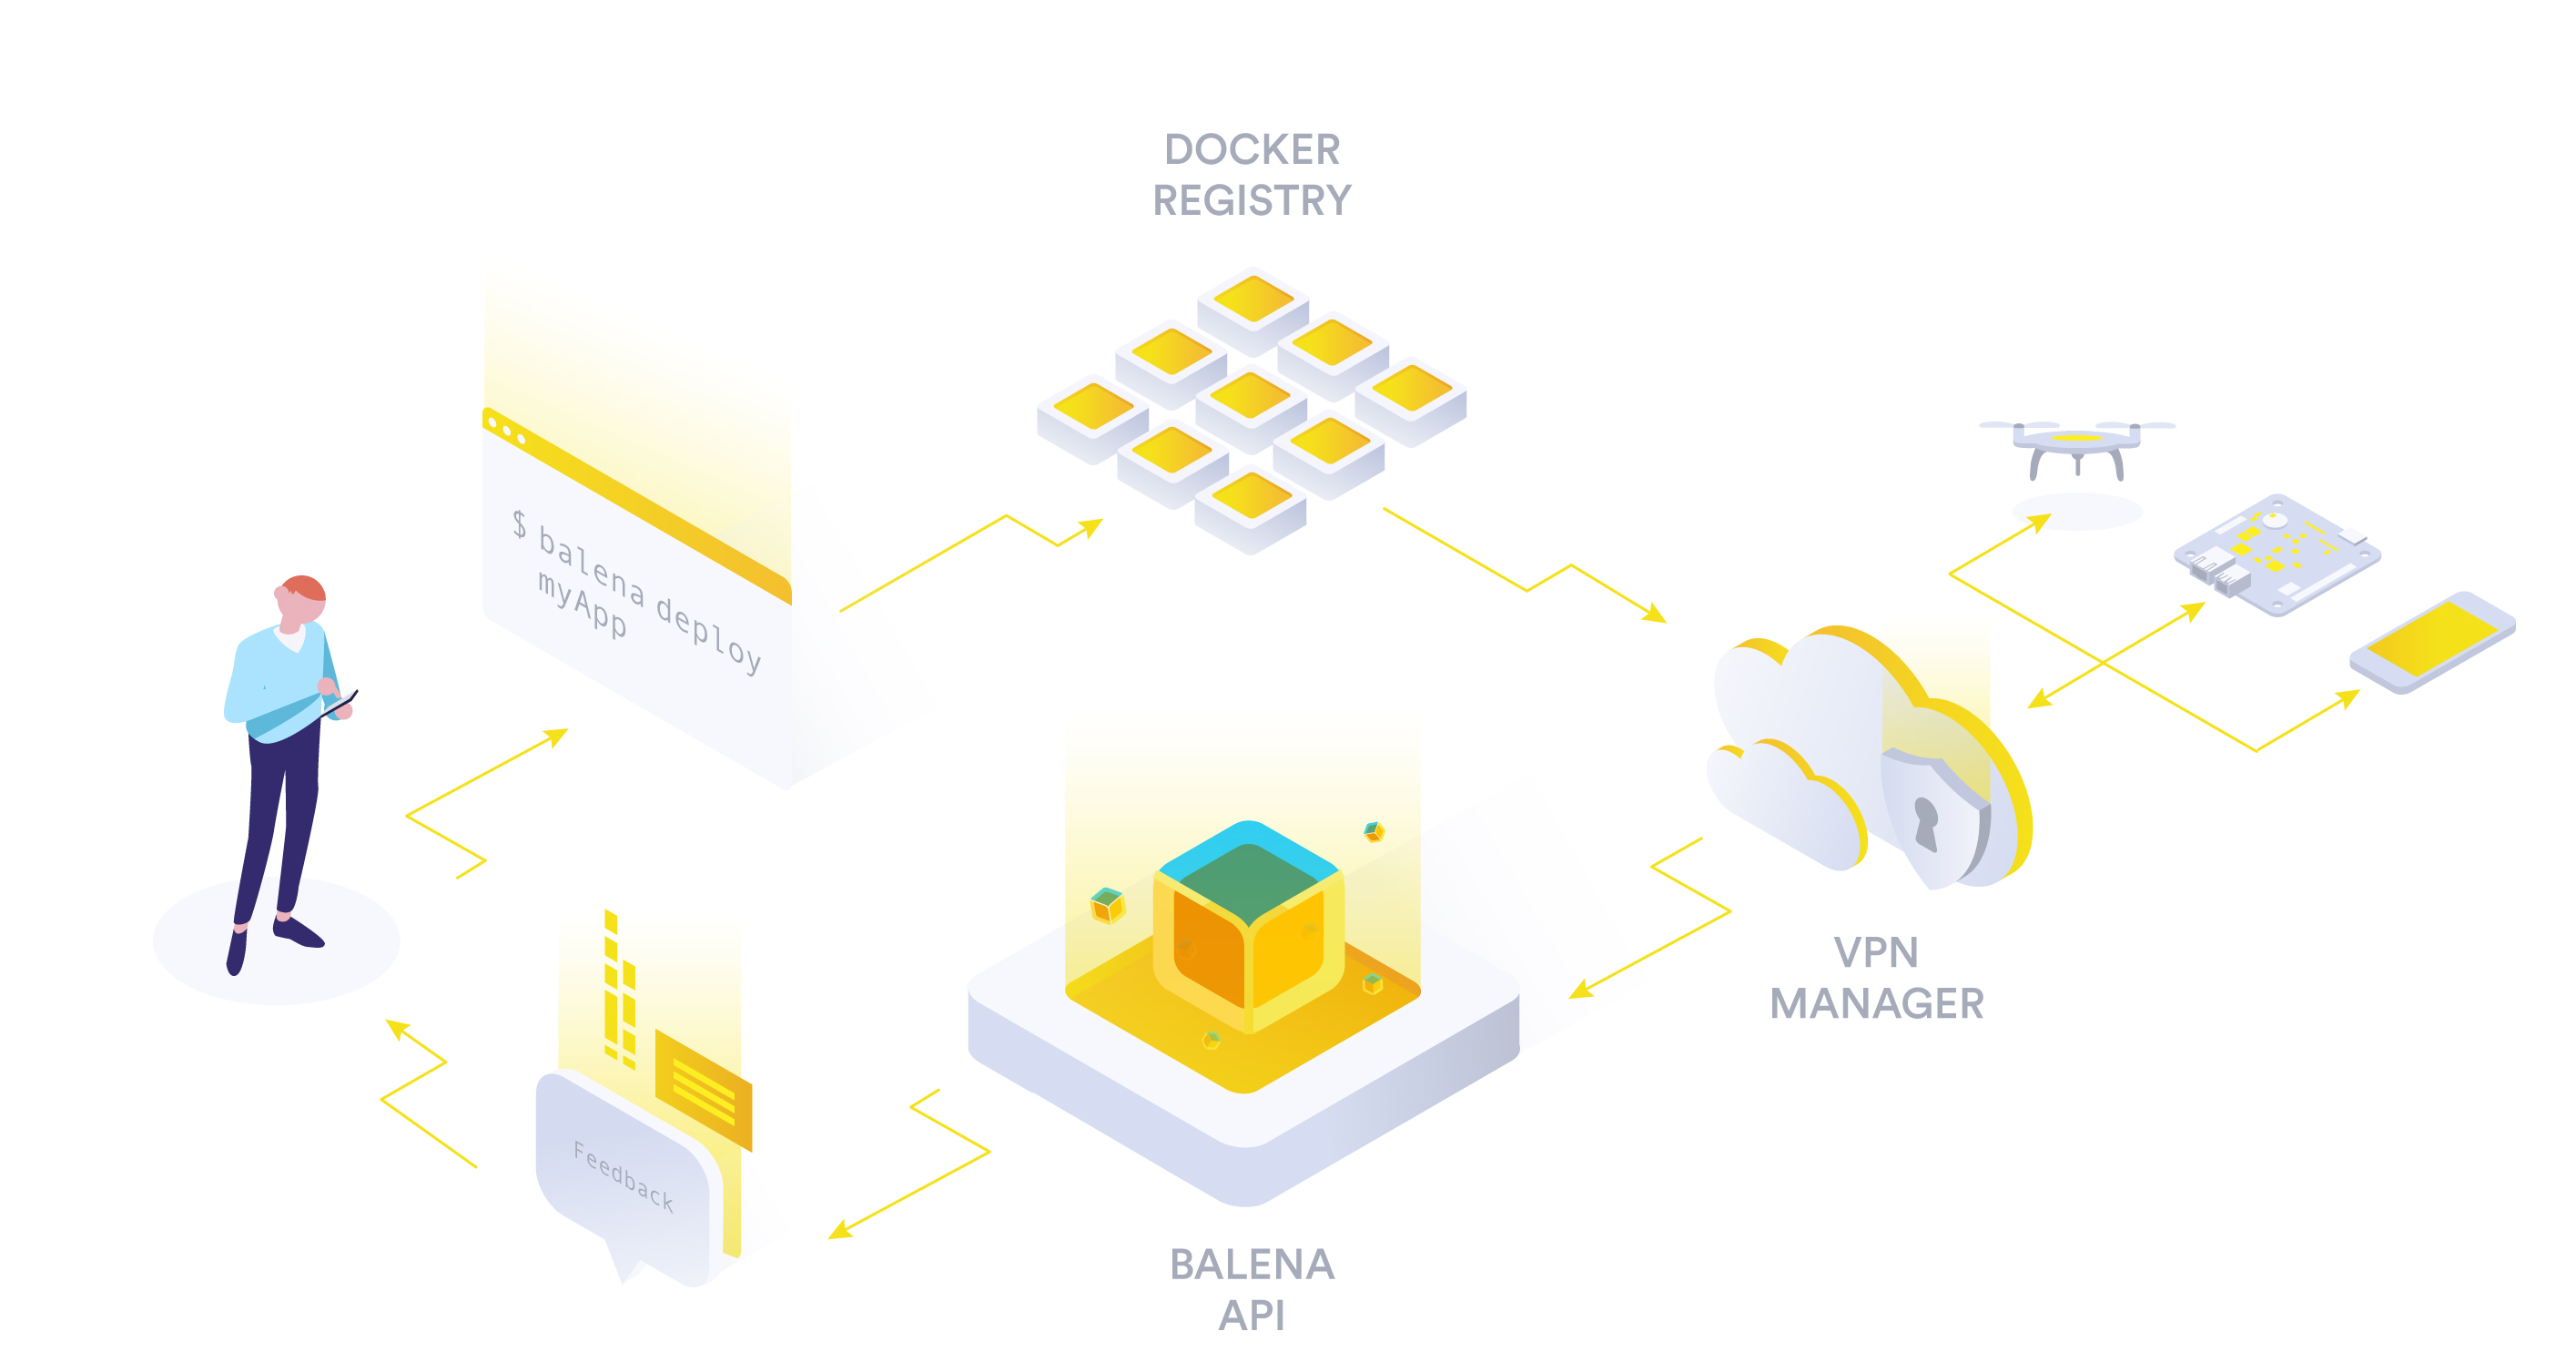
\includegraphics[width=0.9\textwidth]{images/balena_gen_arch.jpg}
    \caption{Overview of the Architecture of Balena Platform \cite{balena}}
    \label{fig:balena_gen_arch}
\end{figure}
\clearpage

Figure \ref{fig:balena_arch} outlines the main components of the balenaOS architecture. Note that the supervisor service rests in a containerized environment, ensuring that it will be able to manage the device and perform critical activities (e.g software update) even in the case of an application crash.

\subsection{Fleet Management using Balena}

The core balena platform, balenaCloud, encompasses device, server, and client-side software, all designed to get your code securely deployed to a fleet of devices. The general idea is that the developer creates an application and pushes it to balenaCloud, then the build servers package the application into containers and deliver them to the balenaOS devices. BalenaOS takes care of running, managing and monitoring the application, while balenaCloud offers on top a web interface to facilitate the fleet management. More in-detail information regarding the balena platform ecosystem can be found on their site\cite{balena}.

Figure \ref{fig:balena_gen_arch} illustrates the above mentioned architecture, where a user pushes the application's code to Builder, which builds it for the Device’s architecture and then ship ready container image binaries to each device.

\section{Decentralized Storage Solution} \label{st:filecoin}

\subsection{Filecoin Architecture} 

Filecoin is a decentralized storage network that turns cloud storage into an algorithmic market. The market runs on a blockchain with a native protocol token which miners earn by providing storage to clients. Conversely, clients spend Filecoin towards miners to store or distribute data (PUT) . The DSN scheme is a tuple of protocols run by storage providers and clients: (GET, PUT, MANAGE). The network architecture \& algorithms are described in the Filecoin White-paper \cite{filecoin-whitepaper}.
 
The Filecoin miners are divided into 2 types. \textbf{Storage Miners} who provide storage to the network (MANAGE) and Retrieval Miners that provide data retrieval to the Network. \textbf{Retrieval Miners} participate by serving data that users request ( GET ). It is natural for Storage Miners to also participate as Retrieval Miners. A high-level overview of how Filecoin works can be seen in Figure \ref{fig:filecoin}.

\begin{figure}[h]
    \centering
    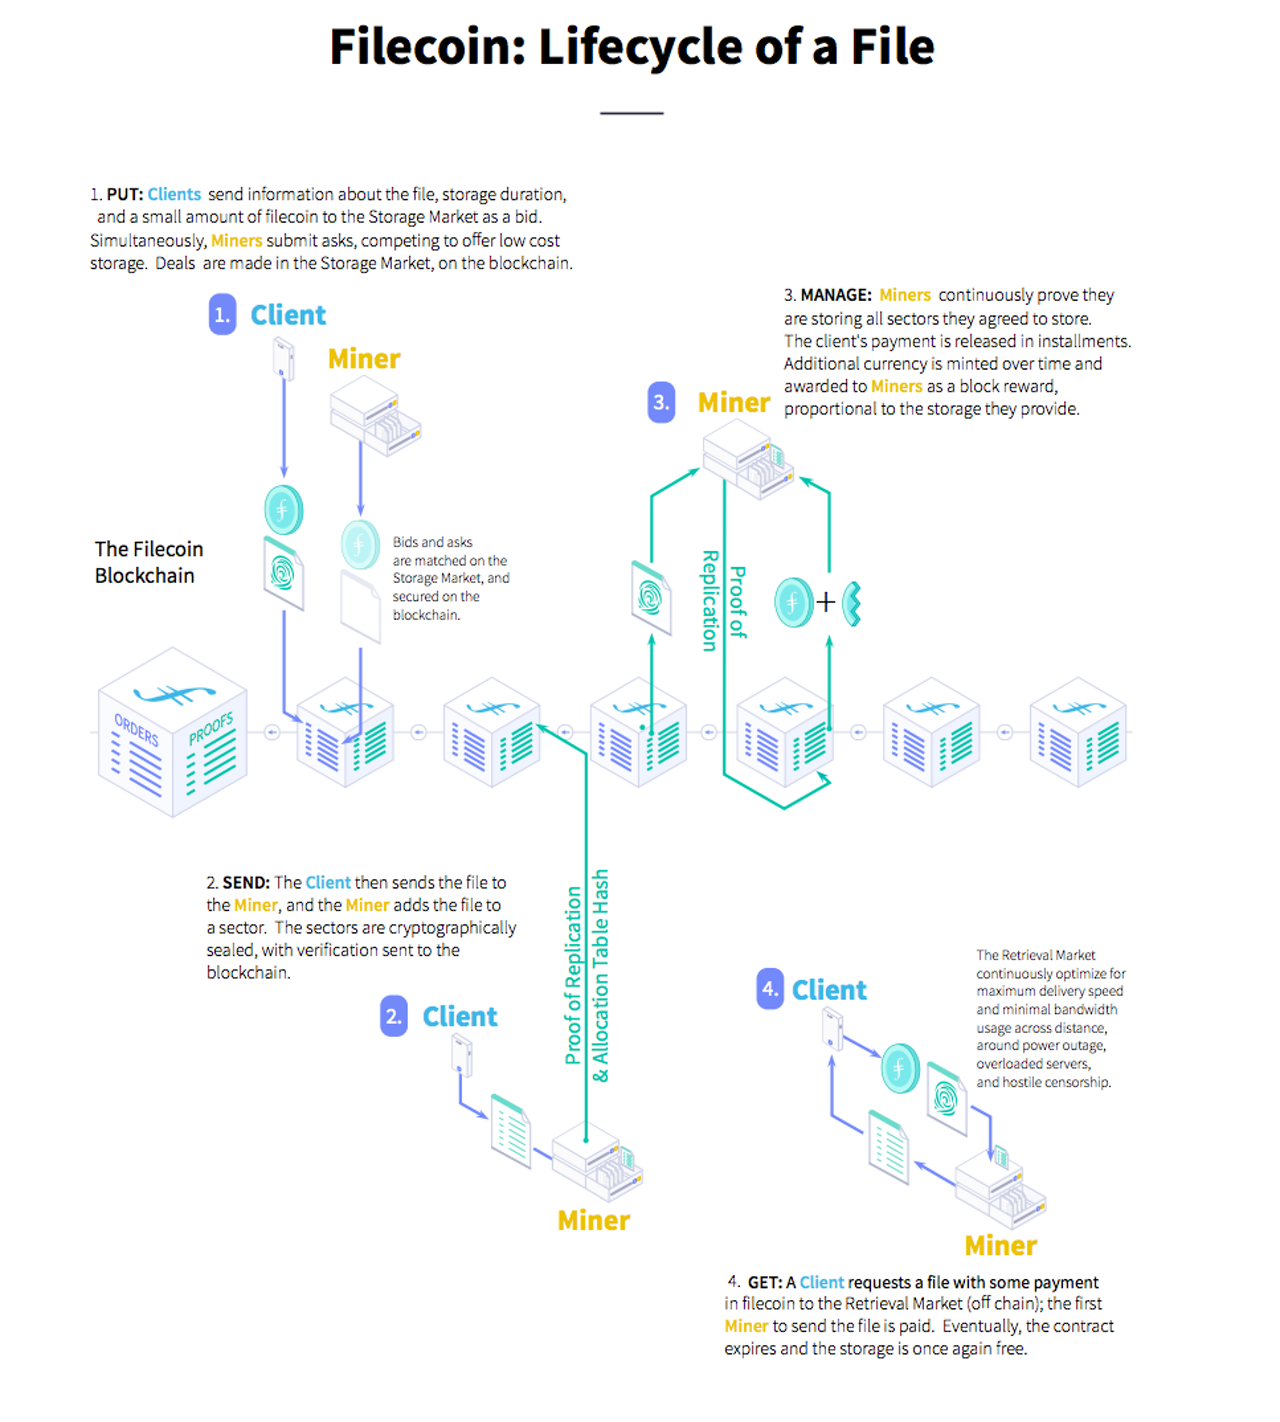
\includegraphics[width=1\textwidth]{images/filecoin.png}
    \caption{The filecoin high level architecture \cite{filecoin-primer}}
    \label{fig:filecoin}
\end{figure}
\clearpage

Filecoin works by creating two decentralized verifiable markets, the \textit{storage market} and the \textit{retrieval market}. Verifiable markets ensure that payment is paid when a specific service has been provided. Moreover, Filecoin introduces two proof-of-storage algorithms, which are used by the network nodes to reach consensus without wasting resources, as with the Proof of Work algorithm. The first algorithm is the proof-of-replication, which allows storage providers to prove that they have stored the data into distinct physical storages, while the second is the proof-of-spacetime algorithm and it allows them to prove that they store a piece of data for a specific amount of time. 

Currently, Filecoin is under heavy development and one could argue that the development progress is at pre-alpha stages, where the foundation is being laid and the protocols are implemented so as Filecoin works in a prototype manner. The markets do not currently function as a dynamic and automated market, but rather in a manual fashion, where a client selects a storage provider from an ask-list and the commits a file to be saved. The storage provider accepts any deal that is proposed from a storage client and matches an ask deal that he has made, regardless the storage it requires. Finally, the network works with devnet FIL that are used for testing purposes and will be reset when the network comes online.

Thus, the proposed Back-End Node participate in the network as both Retrieval \& Storage Miner. By serving as both, it can save locally the data sent by the Edges to the DSN for faster access times. Meanwhile, in Filecoin the data are expected to be saved in multiple locations, providing the necessary data integrity layer that we want. Finally, by participating in the network, the stakeholder’s Cloud will “earn” Filecoin (FIL) that can be used to finance the use of the DSN by the stakeholder’s Edges. Note that Filecoin is expected to have “smart contracts” functionality in the future, enabling thus the system to save for free the data in its own cloud while paying only for the extra copies in other storage providers.

\subsection{Blockchain}

The blockchain is considered to be one of the most groundbreaking innovations of the last decade, foreseeing a completely decentralized future where consensus and \gls{trust} are built upon mathematical models. It is essentially a distributed database of records of transactions - a ledger - where all the nodes in the network participate actively to reach a consensus on the final status of the database. Figure \ref{fig:blockchain} showcases a database which is structured as a chain of blocks, where each block references the last one and encapsulates a number of transactions (database records).  The Merklee Root is the root of Merklee tree (tree of hashes) which can be seen as a succinct proof of the existence of N different elements, in our case transactions. Once a block has been appended to the data structure (ledger), it is impossible to remove or alter it (due to the reference mentioned above). The notion of blockchain  was introduced in 2008 by Satoshi Nakamoto\cite{bitcoin}. It uses well known cryptographic systems, such as public key cryptography\cite{pubkey} and \acrfull{pow}\cite{bitcoin} to create a system where value can be transferred without the need for intermediaries. Bitcoin was the first open source project to implement this new vertical which created the notion of cryptocurrencies. PoW is a process where a computer solves a cryptographic puzzle and is used in various projects, most prominently bitcoin, as a consensus mechanism.

\begin{figure}[h]
    \centering
    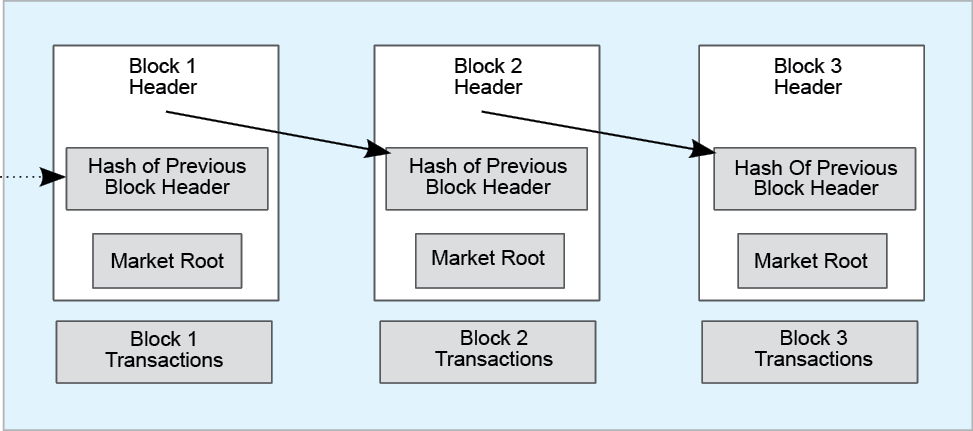
\includegraphics[width=0.6\textwidth]{images/blockchain.jpg}
    \caption{A reference blockchain architecture\cite{opensourceforu}}
    \label{fig:blockchain}
\end{figure}

Finally, blockchain are characterized by 2 important attributes, \gls{permission} and trust. The technology was popularised from projects, such as the bitcoin, explicitly for being permissionless and trustless

\section{Container Migration on balena using Filecoin} \label{st:balena-filecoin}

In the proposed architecture, the “IoT Edge as a service” functionality is provided by running strictly defined services over a pre-agreed amount of IoT Edge device resources. In order to strictly define the resources, the use of docker technology is chosen, containers, in other words, that are acknowledged as units of software that are stateless and atomic (without dependencies). The service customer procures to the service provider a set of containers that will be run when the service contract is activated, at a pre-configured event (or even immediately).

\subsection{Service customer}

For the migration to adhere to the principles of data integrity and high availability, the image containers are stored in the Filecoin Network, always accessible using a unique key, called \textit{CID} in Filecoin and image\_hash in our implementation. The service customer is responsible for ensuring the existence and functionality of the images stored in the network.

In the current version of Filecoin, a file stored in the network can be retrieved  using the file \textit{CID} and the ID of the storage provider with whom the storage deal was made. Thus, each stored file $F$ is characterised by the following tuple $S_f = [CID, miner\_ID]$ and the Service Customer must send a $S_f$ to the Service Provider for each file $F$ that is stored in the network.

\subsection{Service Provider}

The service provider uses the procured CID to request from the Filecoin DSN the files and download them. It downloads a set of containers and a set of corresponding configuration files.

\begin{enumerate}
    \item The images are loaded into balenaEngine using HTTP request to a unix socket that is exposed in the orchestrator container from the balena HostOS. 
    \item The orchestrator uses the supervisor’s API to GET the state of the device’s application. This state is a considerably large data structure in JSON format which describes the entirety of the device, from low-level aspects towards what services run and with what  
    configurations. 
    \item The orchestrator constructs the descriptions of the service customer’s containers according to the schematic of the balena supervisor’s API and the configuration file of each container. As the reader might suspect, each container will use an image that was just loaded to balenaEngine in step (1).
    \item The orchestrator makes a POST request to the supervisor’s API with the device’s state that was GET in step (2), modified to include the service’s state that was generated in step (3).
\end{enumerate}

The above described migration processes is outlined in two distinct Algorithms \ref{alg:algorithm1} and \ref{alg:algorithm2}, from the perspective of service customer (who initiates the process) and the service provider (who finishes the process).

\subsection{Development OS and Local Mode}
The above can only be implemented, with a current version of balenaOS and balenaCloud (or openBalena), if the device uses a development version OS and is configured to work on local mode\cite{localmode}. This is highly important, because a development OS local mode device can manually load images into BalenaEngine and push new releases locally, without the need of BalenaCloud(i.e manually setting the device's \textit{state} using the supervisor API). Having said that, development OS facilitates the development and debugging but exposes the device to serious security risks can \textbf{should not be used in production environments}. Thus, we have concluded that a production ready platform would need to build on top of balenaOS from scratch, with heavy modifications on the supervisor, both of which are open sourced.

\subsection{A centralized interim solution \textit{(perhaps)}}

With the above solution, we strived for the autonomy of the IoT Edge device, having zero dependencies when functioning as a service provider, especially when providing a fault-tolerance insurance.

But, it is possible to simplify the above process, by using a back-end cloud system where Balena-CLI is installed. Then, using a simple web application that will function as a simple HTTP RESTful API for the Balena-CLI, we could follow the following approach:

\begin{enumerate}
    \item Instead of downloading the images locally, instruct the backend to download the service customer’s images from the filecoin DSN.
    \item GET the docker-compose.yaml file from the BackEnd.
    \item Append the service customer’s service into the docker-compose.yaml file downloaded in step (2), according to the specifications found in the configuration file.
    \item Make a POST request to the back-end and upload the new docker-compose.yaml.
    \item Instruct the backend to run the command “\texttt{balena push <application\_name>}".
\end{enumerate}

The configuration files describe the settings that are needed for the containers to function properly (e.g exposed ports). Currently,  the configuration file also dictates the contract activation clauses, indicating to the orchestrator when the services will need to start, as well as the Filecoin storage provider(miner) ID. The contract clauses are expected to exist in a separate contract data structure which also will define the system resources that will be provisioned for the services. An example of the configuration file can be found in Figure \ref{fig:configuration-file}.

\begin{figure}
\centering
\begin{minted}[%
 breaklines,
 mathescape,
 linenos,
 numbersep=5pt,
 frame=single,
 numbersep=5pt,
 xleftmargin=0pt
 ]{json}
    {
    "service_customer_id":"EdgeX-64",
    "serviceName": "nodered-device-service",
    "activationEvent": "offline",
    "event":{
        "interval": "20",
        "ip":"https://f223871f69c8b68a509868943f84bf7b.balena-devices.com/"
    },
    "ports": "1880",
    "volumes": "node-red-data:/data",
    "depends_on":["lora-appserver","edgex-core-command", "edgex-core-data","edgex-core-consul","orchestrator"],
    "miner_address": "t1hieq4dc3y3tlptg3xy2nb4ruczlomcixak2we4a"
}
\end{minted}
\caption{Reference structure of the configuration.json file}
\label{fig:configuration-file}
\end{figure}

\begin{algorithm}
% \begin{algorithmic}[1]
Build container image $C_j$ from Dockerfile\;
Create configuration.json  $Y_j$ \;
Upload container image $C_j$ to Filecoin DSN\;
   $X_j$  $\leftarrow$ container image File CID \;
Upload configuration file $Y_j$ to Filecoin DSN\;
   $Y_j$ $\leftarrow$ configuration file CID \;
Send $X_j$ to Service Provider\;
Send $Y_j$ to Service Provider\;
% \end{algorithmic}
\caption{Algorithm  1 Migration - Preparation. Actor: Service Customer}
\label{alg:algorithm1}
\end{algorithm}

\begin{algorithm}

Download image $I_j$ from Filecoin DSN using $X_j$ \;
Download configuration file $C_j$  from Filecoin DSN using $Y_j$ \;
configuration $\leftarrow$ $C_j$ \;
event\_type $\leftarrow$ configuration.event\_type  \;
event\_conditions $\leftarrow$ configuration.event\_conditions \;
service\_name $\leftarrow$ configuration.service\_name \;
Load $I_j$ $\rightarrow$  balenaEngine \;
Set supervisor state \;
\While {contract is active}{
    event $\leftarrow$ current event\;
    \eIf {event is in contract\_event and event\_conditions are true}{
        Start service (service\_name input) \;
        Break \;
    }{
    Continue \;
    }
}
\caption{Algorithm 2 Migration. Actor: Service Provider}
\label{alg:algorithm2}
\end{algorithm}
\clearpage

\begin{sidewaysfigure}
    \centering
    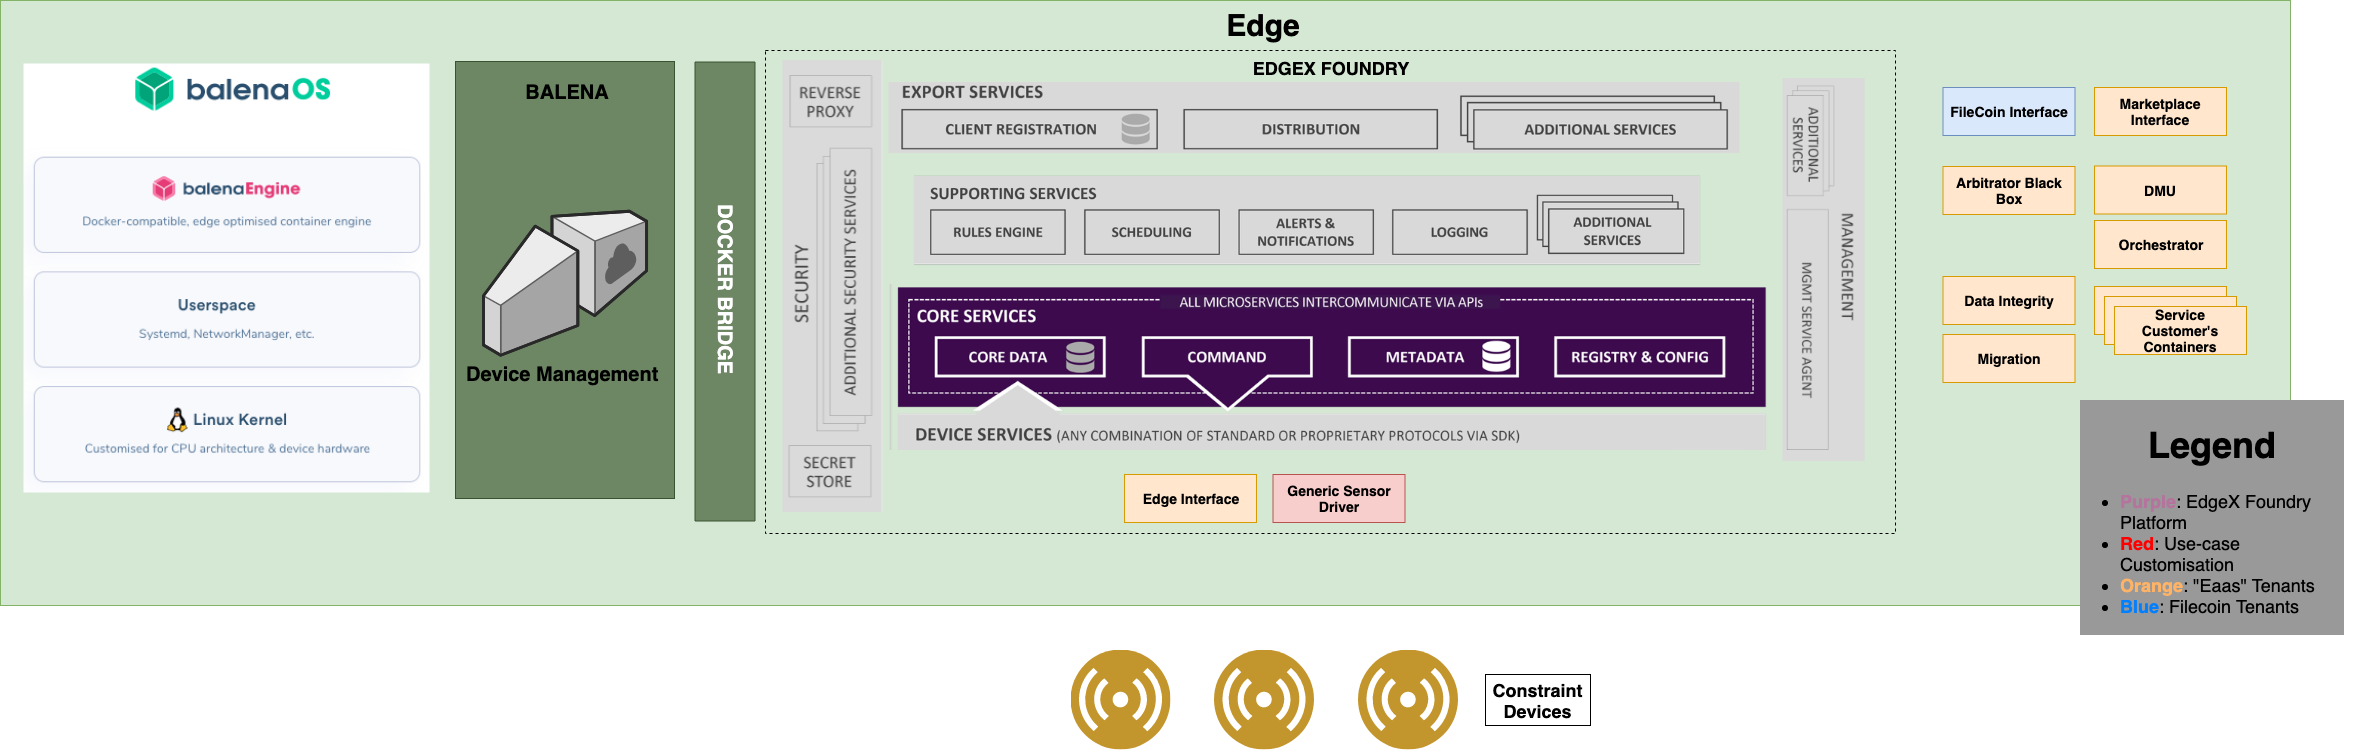
\includegraphics[width=1\textwidth]{images/EdgeArch_v7.png}
    \caption{The high level proposed architecture of an IoT Edge device}
    \label{fig:edge}
\end{sidewaysfigure}

\section{IoT Edge Architecture}

The IoT Edge can have different forms depending on the IoT application needs, ranging from a micro-computer with industry standards, to even a micro Data Center to support computational demanding localised AI services. Although the number of IoT Edge devices and their computational power can differ considerably, our architectural approach is relevant without altering the core functionality and the unique features that we envisage to support.
 
In order to create a highly modular and robust system, we turned to the microservices paradigm adjusted for the needs and abilities of the Edge. Following the principle of loosely-coupled services, each service is placed in its own container, even those belonging to the same platform (e.g EdgeX Foundry). The containers communicate through HTTP REST calls using Docker Bridges and each container will be configured appropriately for the service it hosts. As such, services that handle hardware or need Internet Access will have more \textit{“access control rights”} than other services. An overview of the architecture is shown in Figure \ref{fig:edge}.

\subsection{IoT Edge Architecture reference services}
\begin{enumerate}
    \item \textbf{"IoT Edge as a service” Modules}
    \begin{enumerate}[label*=\arabic*.]
        \item \textbf{DMU:} This service is responsible for evaluating the contracts in the IoT Edge Marketplace. Whether concerning an offer or the parameters of a demand. The simplest form is rule-based.
        \item \textbf{Arbitrator:} The service that is responsible for ensuring that every party in an service contract act as a trusted party.
        \item \textbf{Migration:} The service responsible for uploading \& downloading the necessary images in the DSN.
        \item \textbf{Edge2Edge Interface:} The service is responsible for inter-Edge communication.
        \item \textbf{Orchestrator:} Responsible for managing and overseeing the service provision process.
        \item \textbf{Marketplace Interface:} A Restful API that is responsible for probing the marketplace and fetching information from it (i.e offers).
        \item \textbf{Service Customer Containers:} All the containerized services of the service customer that remain idle until their activation by the orchestrator.
        \end{enumerate}
    \item \textbf{Filecoin Modules:}
        \begin{enumerate}[label*=\arabic*.]
        \item \textbf{Filecoin Interface:}  This service is responsible for connecting with the Filecoin network, uploading \& downloading the necessary content.
        \end{enumerate}
\end{enumerate}

\subsection{IoT Edge Platform}

Our approach for the IoT Edge is to expand an existing solution with services that will enable it to offer the envisaged functionalities of our proposal. The main platform chosen to be responsible for performing much of the usual IoT Edge functionality, as already mentioned, is EdgeX Foundry.

\subsection{Device Management at the Edge}

The role of device management is realised by Balena. The host OS is responsible for kicking off the device supervisor, balena’s agent on a device, as well as our containerized services. Within each service's container we can specify a base OS, which can come from any existing Docker base image that is compatible with our device architecture.  

\subsection{Data Integrity at the Edge}

Data Integrity is considered a key aspect of the proposed design. It ensures the overall completeness, accuracy and consistency of data. This can be indicated by the absence of alteration between two instances or between two updates of a data record, meaning data is intact and unchanged.
 
Data Integrity will be enforced from end-to-end, from the IoT Edge that aggregates sensor data to the cloud that serves them. We consider a scheme where each IoT Edge has a unique private key generated at a setup phase, unknown to the centralized Cloud Back-End, that is used as a unique device signature.
 
As per the Edgex architecture, the data integrity service will receive the sensor data from the distribution service in the export services layer. The service then will create a certain proof (e.g. hashing) of a certain unit of data. This proof will be publicly accessible and auditable, say by publishing it in a blockchain or storing in it Filecoin and publicly announcing the key to retrieve it. Thus, if the integrity of the data is requested, the cross-checking of the proof and the data themselves will provide the necessary integrity. 

We feel that there is no need to strictly define the integrity module as it attributes can change depending on the use-case of the IoT Edge device. Critical infrastructure could demand a more thorough and secure fashion, which impedes ease of use and efficiency but more common applications could opt for a better user-experience.
 
One could argue that the data integrity process should be embedded in the core data service, which functions as a centralized gateway for all sensor data in the Edgex platform, but we estimate that we can implement it as an add-on. This is due to the fact that Edgex services are considered as tamper-proof from the user, thus trusted. As they are trusted, they will function as we expect them to and as a result, they will  certainly propagate the data to the data integrity add-on service to construct the proof.
 
On top of that, Filecoin ensures that the data will securely be stored in multiple physical storage locations and thus will not have a single point of failure. In each Edge, the Filecoin Interface Module will package the data needed to be delivered and will make a bid order in the Filecoin Storage Market. The IoT Edge will provide to the Cloud Back-End the necessary keys in order to access the data in the DSN for various purposes (i.g analytics, history, etc. ).  

Finally, we underline that the IoT Edge device owner must be able to finance the use of the Filecoin network, either buying FIL in the market (i.e through exchanges) or using his Cloud Back-End as Filecoin miner. The exact economics and cost analysis are outside the scope of the Thesis and impossible to determine, as the Filecoin network hasn’t launched as of September 2019.
 
\subsection{Fault-Tolerance}

At specific arbitrary occasions, the IoT Edge will begin the process in order to find another IoT Edge device that will serve as the insurance provider. The insurance provider will not only hand-over the devices of the IoT Edge but will also perform any pre-processing or other arbitrary activity. 

The Nodes (IoT Edge Devices) can participate in a centralized IoT Edge Market where Stakeholders can find service-providers or offer their cloud as a Sibling. A service-provider (or more specifically, insurance-provider) is an IoT Edge that has made a specific contract with another IoT Edge to serve as a backup server in case of critical failure. Although the offered services can vary, the main responsibilities are expected to be: 1)Constrained devices handover 2) Data preprocessing 3) North-side data forwarding.

The IoT Edge Market is a centralized service offered by the system’s manufacturer or a IoT Edge federation. It offers the possibility for cloud to find available IoT Edge and then negotiate directly. The Decision Making Unit (DMU) reviews offers, either as customer or provider, and decide on their prospect. If agreement is reached, the central system is informed and the IoT Edge Arbitrators create the contract and inform the central arbitrator authority.
 
Fault-Tolerance is presented in detail in the Section \ref{st:fault-tolerance} .

\section{Cloud Layer Architecture}

While neither the implementation, nor the architecture focuses on the cloud layer architecture, we believe that it is worth giving the general gist of the architecture, in order to outline the holistic approach of our architecture regarding both layers (Edge, Cloud).

\begin{figure}[h]
    \centering
    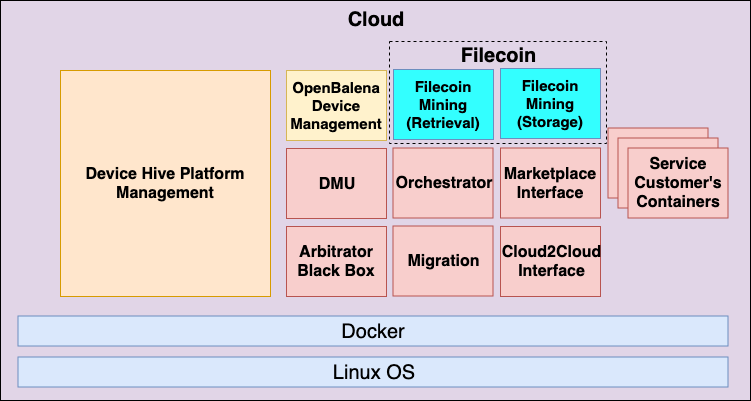
\includegraphics[width=0.9\textwidth]{images/CloudArch_v6.png}
    \caption{High level overview architecture of a Cloud system}
    \label{fig:cloud}
\end{figure}

The system generally follows the paradigm of an IoT platform, using a central Back-End to orchestrate various IoT Edge devices, aggregate data, perform heavy computations, analytics and offer interfaces for 3rd party services or for the system admin. The Cloud Module belongs to a larger network of Cloud Nodes that participate in a service marketplace offering or demanding the computational resources, much like in the IoT Edge architecture .Thus, we can consider the Cloud Module as a Back-End Node in a Graph of relatively homogeneous (software-wise) Systems.
 
The architecture is agnostic on the specific hardware or cloud solution, but we project common infrastructure in a linux server distribution, such as Ubuntu or Debian. The architecture follows the microservices paradigm and the intercommunication is done using Docker bridges and the HTTP protocol (RESTful APIs). The necessary infrastructure for the various services (such as registry, message bus, etc.) is offered by the reference core platform, DeviceHive\cite{devicehive}. The architecture is shown in Figure \ref{fig:cloud}.

\subsection{Cloud Architecture reference services}

\begin{enumerate}
    \item \textbf{"IoT Edge as a service” Modules:}
    \begin{enumerate}[label*=\arabic*.]
    \item \textbf{DMU:} This service is responsible for evaluating the contracts in the Cloud Marketplace, whether concerning an offer or the parameters of a demand. The simplest form is rule-based.
    \item \textbf{Arbitrator:} The service that is responsible for ensuring that every party in an insurance contract is a trusted party.
    \item \textbf{Migration:} The service responsible for uploading \& downloading the necessary images in the DSN.
    \item \textbf{Cloud2Cloud Interface:} The service is responsible for inter-cloud communication.
    \item \textbf{Orchestrator:} Responsible for managing and overseeing the service provision process.
    \item \textbf{Marketplace Interface:} A Restful API that is responsible for probing the marketplace and fetching information from it, such as offers.
    \item \textbf{Service Customer Containers:} All the containerized services of the service customer remain idle until being activated by the orchestrator.
    \end{enumerate}
    \item \textbf{Filecoin Modules:}
     \begin{enumerate}[label*=\arabic*.]
     \item \textbf{Filecoin Interface:}  This service is responsible for connecting with the Filecoin network, uploading \& downloading the necessary content.
    \end{enumerate}
    \item \textbf{IoT Edge Platform Management \& Device Management services}
 \end{enumerate}  

\subsection{IoT Edge Platform Management}
    The IoT Edge Platform Management is responsible for aggregating the data from the IoT Edge devices (uplink), issuing (downlink) commands relevant to their functionality (e.g. activating an actuator, etc.) and offering services (e.g. analytics) to users and 3rd party services. Moreover, the IoT Edge Platform Management provides the necessary infrastructure (e.g message bus), for all the cloud Modules to communicate with other Modules or Systems.
    
    There are numerous platform management solutions coupled with production ready infrastructure and services, such as Google IoT, AWS IoT Core, Microsoft Azure, etc. We have focused our research on Open Source Solutions that are characterized by maturity, vibrant community as also modularity. The platform of choice to use as a reference is DeviceHive, as it offers unique modularity and is structured as an array of containerized microservices. Device Hive also serves as a proxy with the south side (Edge) using a multitude of available protocols (HTTP REST, MQTT, CoAp, etc.).
    
\subsection{Fleet Management}
As described in the IoT Edge section, the fleet management solution is Balena, but instead of using the payed service provided by Balena.io, we will be using the Open Source solution OpenBalena that will be hosted in the Back-End Node. The service is responsible for offering the Balena Dashboard, building and serving the container images to the Edges, provisioning new IoT Edge devices and performing OTA (Over-the-Air) updates.

\subsection{Platform Management vs Device Management}
We consider platform management as the process of managing the various functionalities and services of the IoT Edge devices, such as aggregating data, performing analytics, controlling actuators, etc. Fleet management is the process of managing the IoT Edge themselves, provisioning new devices, performing Updates Over Air (OTA), maintenance, etc.

\subsection{Fault-Tolerance}
The structure of the Fault-Tolerant group of Modules is similar to the Edge’s. The Nodes (Cloud modules) can participate in a centralized Cloud Market where Stakeholders can find service-provider s or offer their cloud as a Sibling. A service-provider is a cloud that has made a specific contract with another cloud to serve as a backup server in case of critical failure. Although the offered services can vary, the main responsibilities are expected to be: 1)IoT Edge systems hand-over 2)data processing 3)API for 3rd party services and many more custom tailored services.
 
The Cloud Market is a centralized service offered by the system’s manufacturer or a cloud federation. It offers the possibility to the cloud to find available service-providers and then negotiate directly. The service-provider Decision Making Unit (DMU) reviews offers, either as customer or provider, and decide on their prospect. If agreement is reached, the central system is informed and the Arbitrators create the contract and inform the central arbitrator authority.
 
Fault-Tolerance is presented in detail in the Section \ref{st:fault-tolerance}.

\section{Sensor Layer}
The proposed architecture exploits the unique features of Edgex, namely its extreme modularity and customizability. As mentioned above, the containerized microservices architecture enables both the system provider and the stakeholder to equip the IoT Edge Node with literally any sensor or constraint device that the hardware can support. As such, we are completely agnostic in regards to the nature of the sensor as long as the device service that handles that particular sensor follows the Edgex specifications.

It is pertinent to mention that the Sensor Layer is prone to cyber and physical attacks, both because of easy physical access (usually) and because of low processing power which results in limited cryptographic functionalities. Nonetheless, our architecture is Sensor Layer agnostic and thus such an analysis falls outside of the scope.

\begin{sidewaysfigure}
    \centering
    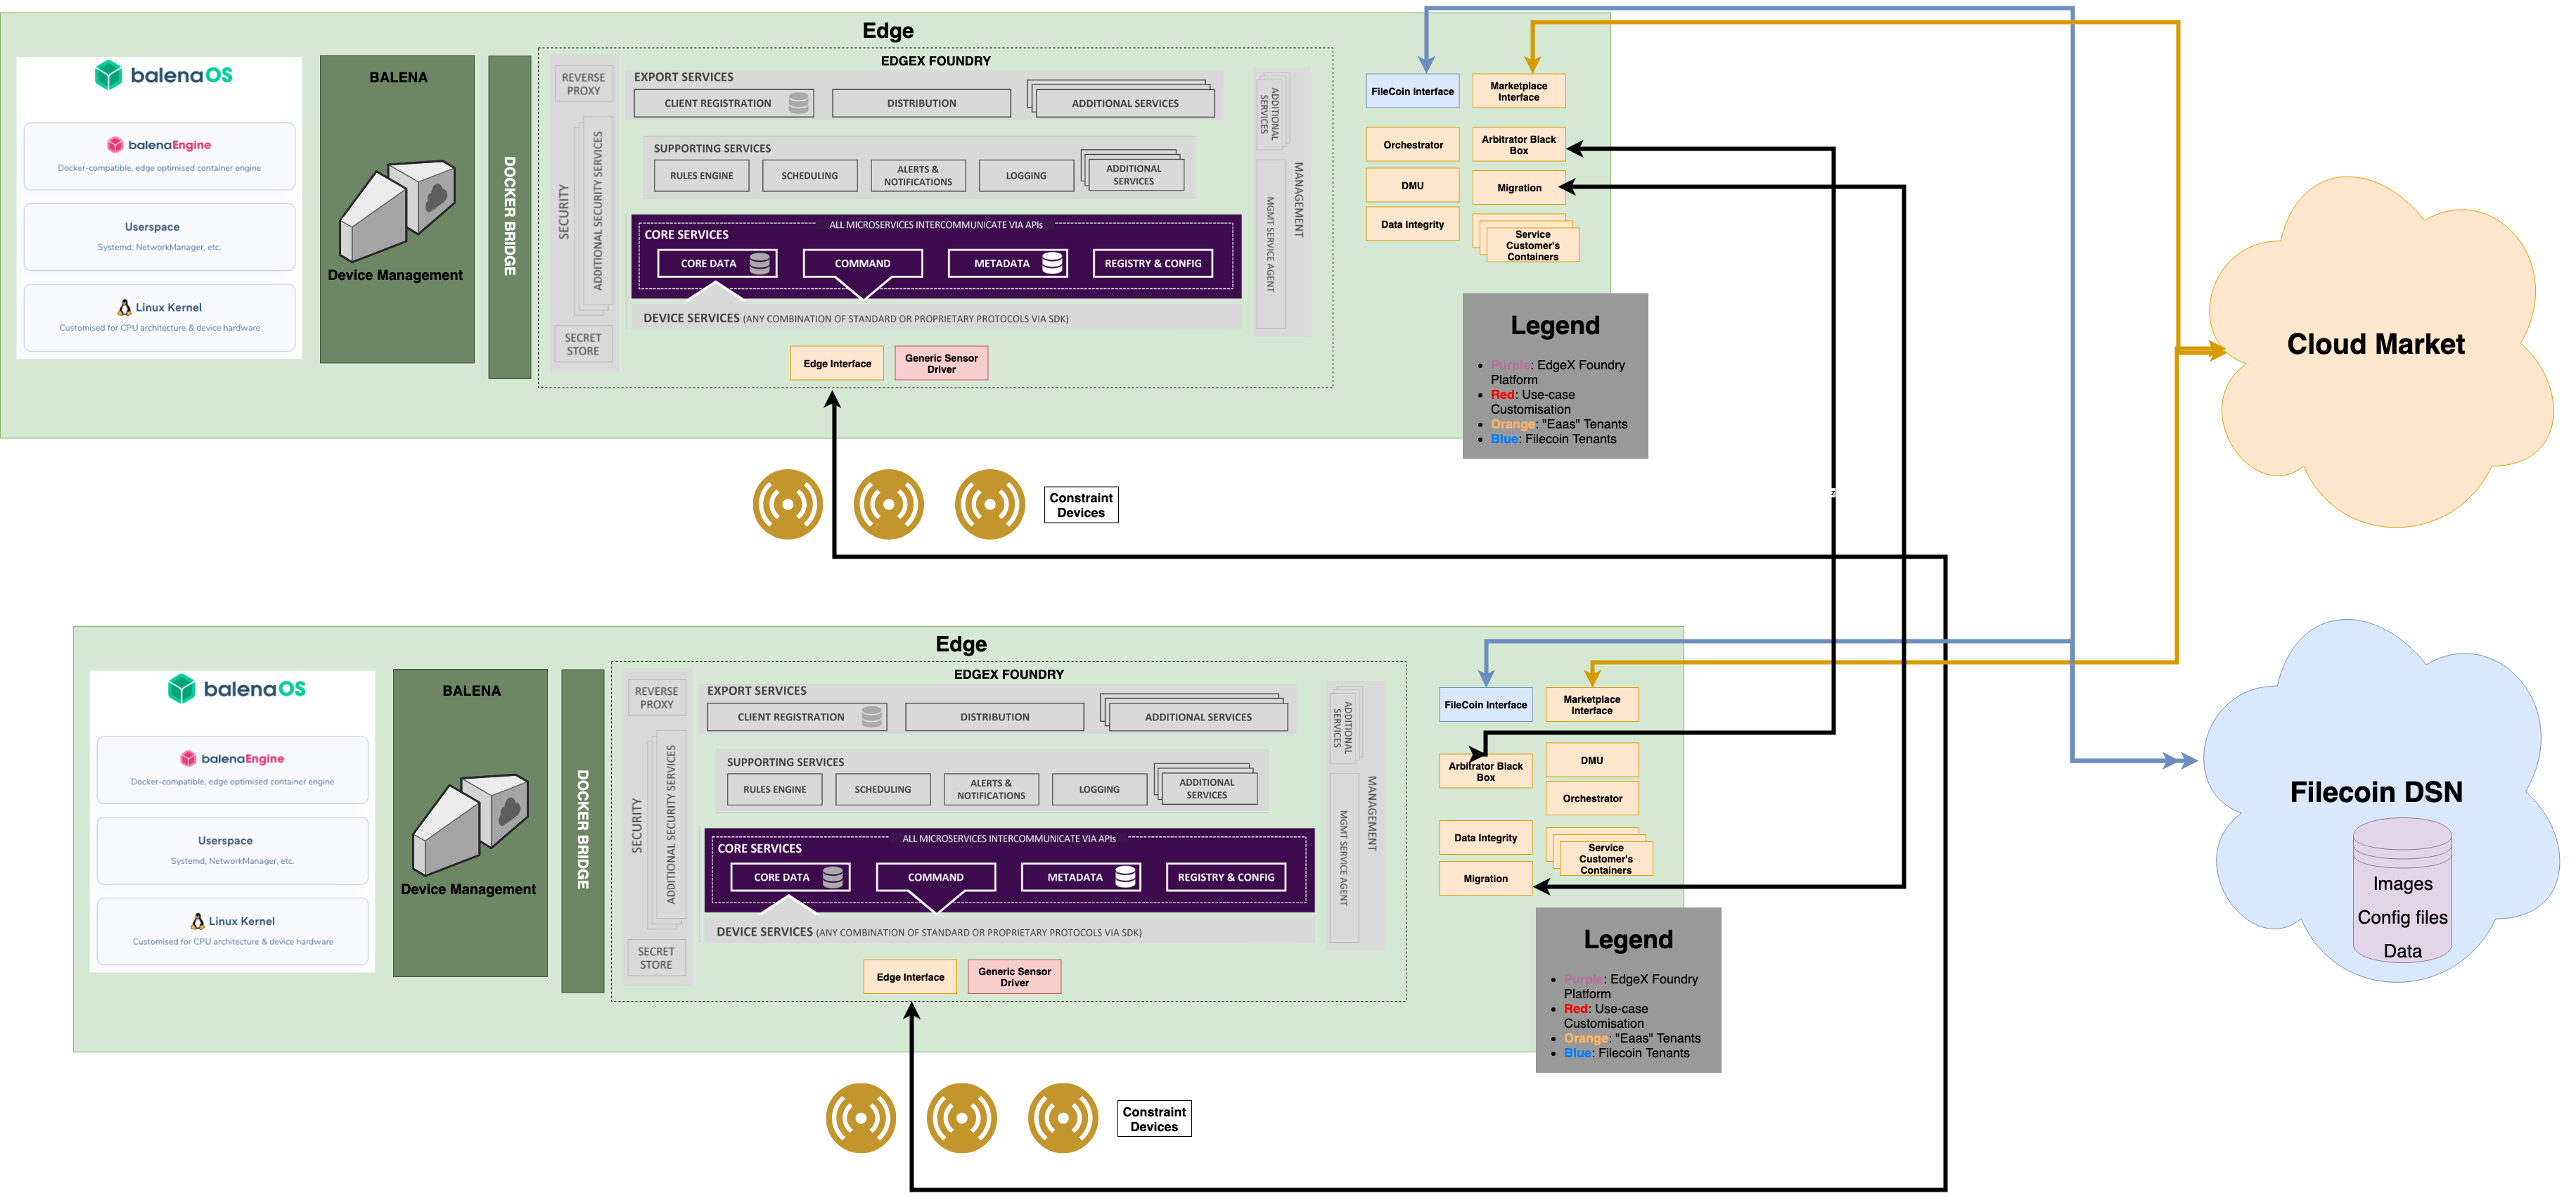
\includegraphics[width=0.9\textwidth]{images/EdgeEdgeArch_v2.png}
    \caption{Diagram showcasing the communication between microservices of different IoT Edge devices}
    \label{fig:edge2edge}
\end{sidewaysfigure}
\clearpage
\section{Communication Principles}
\subsection{IoT Edge to Edge}

In the proposed design, the IoT Edge devices are able to communicate automatically, in order to collaborate, offer insurance policies and even exchange resources for value.
 
The intercommunication is conducted through the south bridge of the Edge, using the Edgex platform as interface. As Edgex is hardware and protocol agnostic, the architecture enforces this paradigm and the interface will not be tied to a specific hardware protocol solution. It is expected to use a wireless protocol (e.g NB IoT, cellular data, WiFi, etc.) with certain (\textit{R})ange, \textit{(B)}andwidth, \textit{(P)}ower \textit{(C)}onsumption \textit{(R, B, PC)} requirements, featuring a different set of \textit{(R, B, PC)} according to the specification for each use-case and IoT Edge capabilities. The Interface module is built according to the Device Service specification of the Edgex platform using their SDK.
 
In essence, the interface module is the low-level connectivity layer of the Edge to Edge communication. It will expose a REST interface to the rest of the services that are interested in communicating with other IoT Edge devices, effectively acting as a gateway and reverse-proxy.

By abstracting the communication protocol, the architecture enables interoperability between the same IoT Edge modules and completely different communication protocols, depending on the use-case and the IoT Edge devices.

Figure \ref{fig:edge2edge} gives an impression on the communication between Edges. The arrows connect the submodules or subsystems that are expected to communicate using HTTP requests and RESTful APIs. For example, the Filecoin interface module is expected to communicate directly with the Filecoin network. Arrows that pass through the IoT Edge Interface indicate that they use the interface as a gateway.
\subsection{Cloud to Edge}

Each microservice in the IoT Edge platform has a corresponding one situated at the Cloud, which performs the same functionality. These two are expected to communicate directly. For example, EdgeX and DeviceHive have the same functionality in their respective systems, as platform managers performing the reference IoT activities related to the aggregated IoT data, thus they communicate directly.

Figure \ref{fig:cloud2edge} shows the communication between an IoT Edge and it’s corresponding Cloud, the arrows connect the submodules or subsystems that are expected to communicate using HTTP requests and RESTful APIs.
\clearpage
\begin{sidewaysfigure}
    \centering
    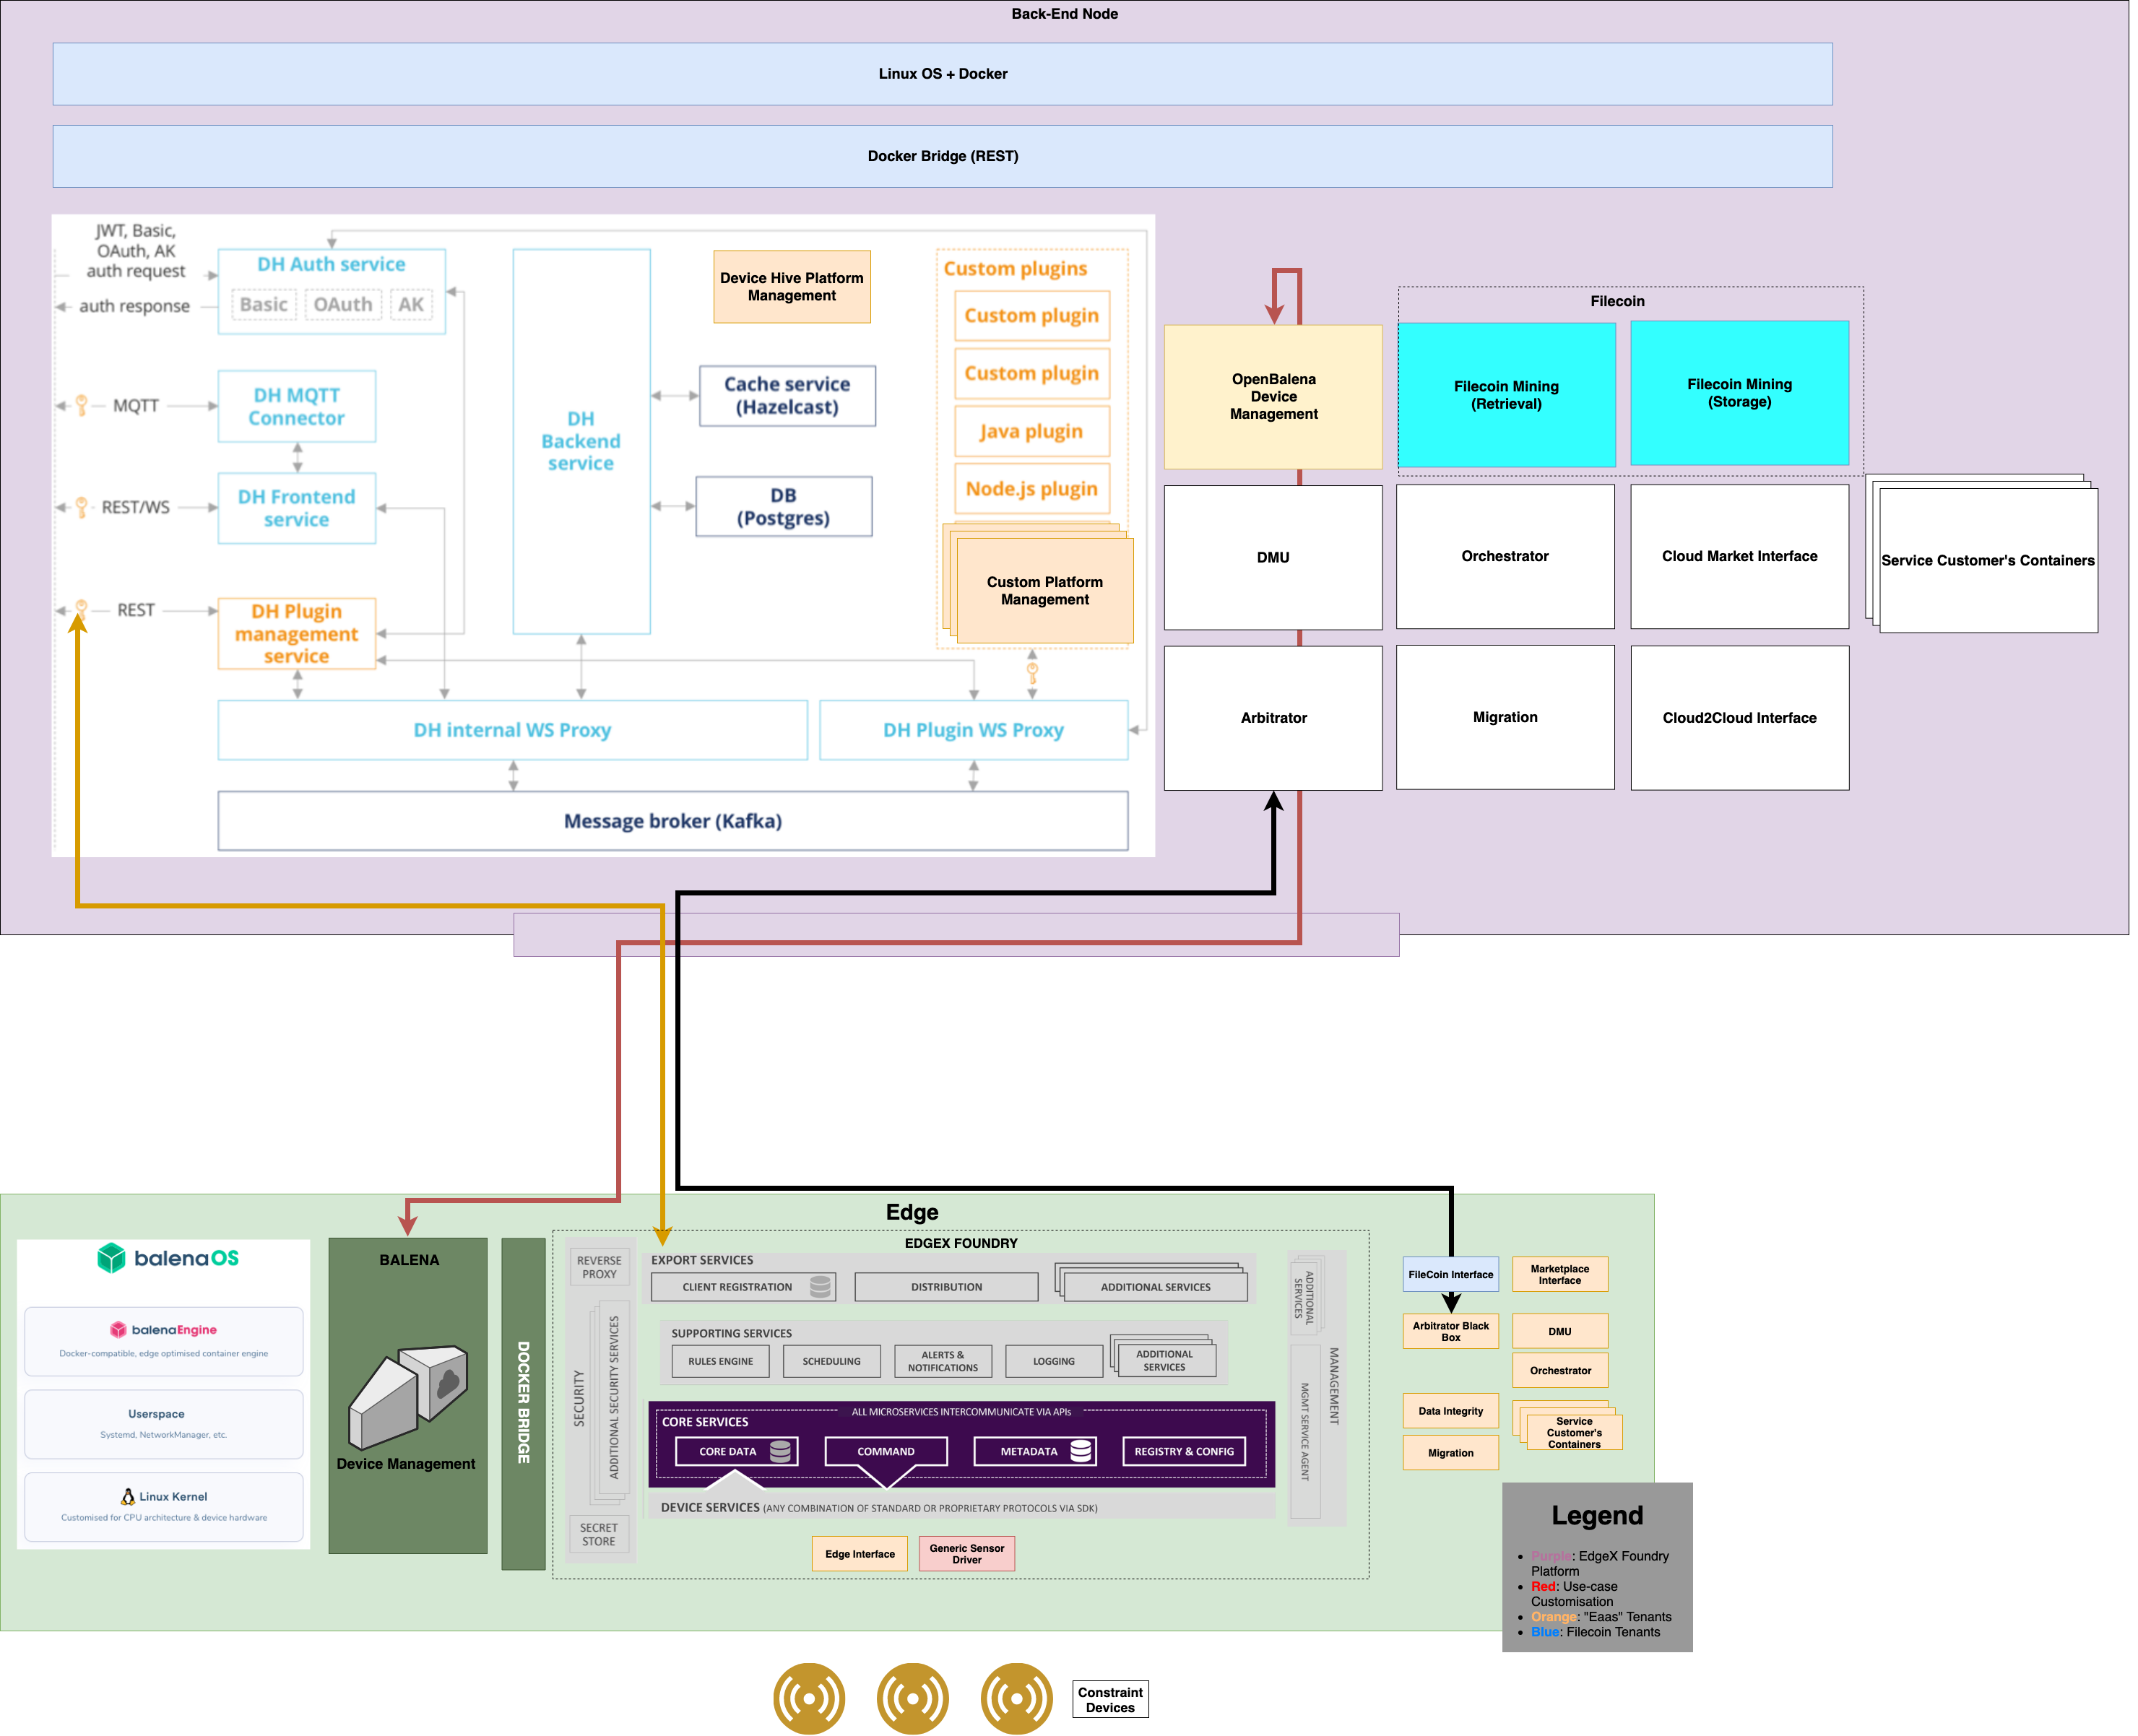
\includegraphics[width=0.7\textwidth]{images/CloudEdgeArch_v4.png}
    \caption{Diagram showcasing the communication between microservices of an IoT Edge device and it's parent Cloud}
    \label{fig:cloud2edge}
\end{sidewaysfigure}

\begin{sidewaysfigure}
    \centering
    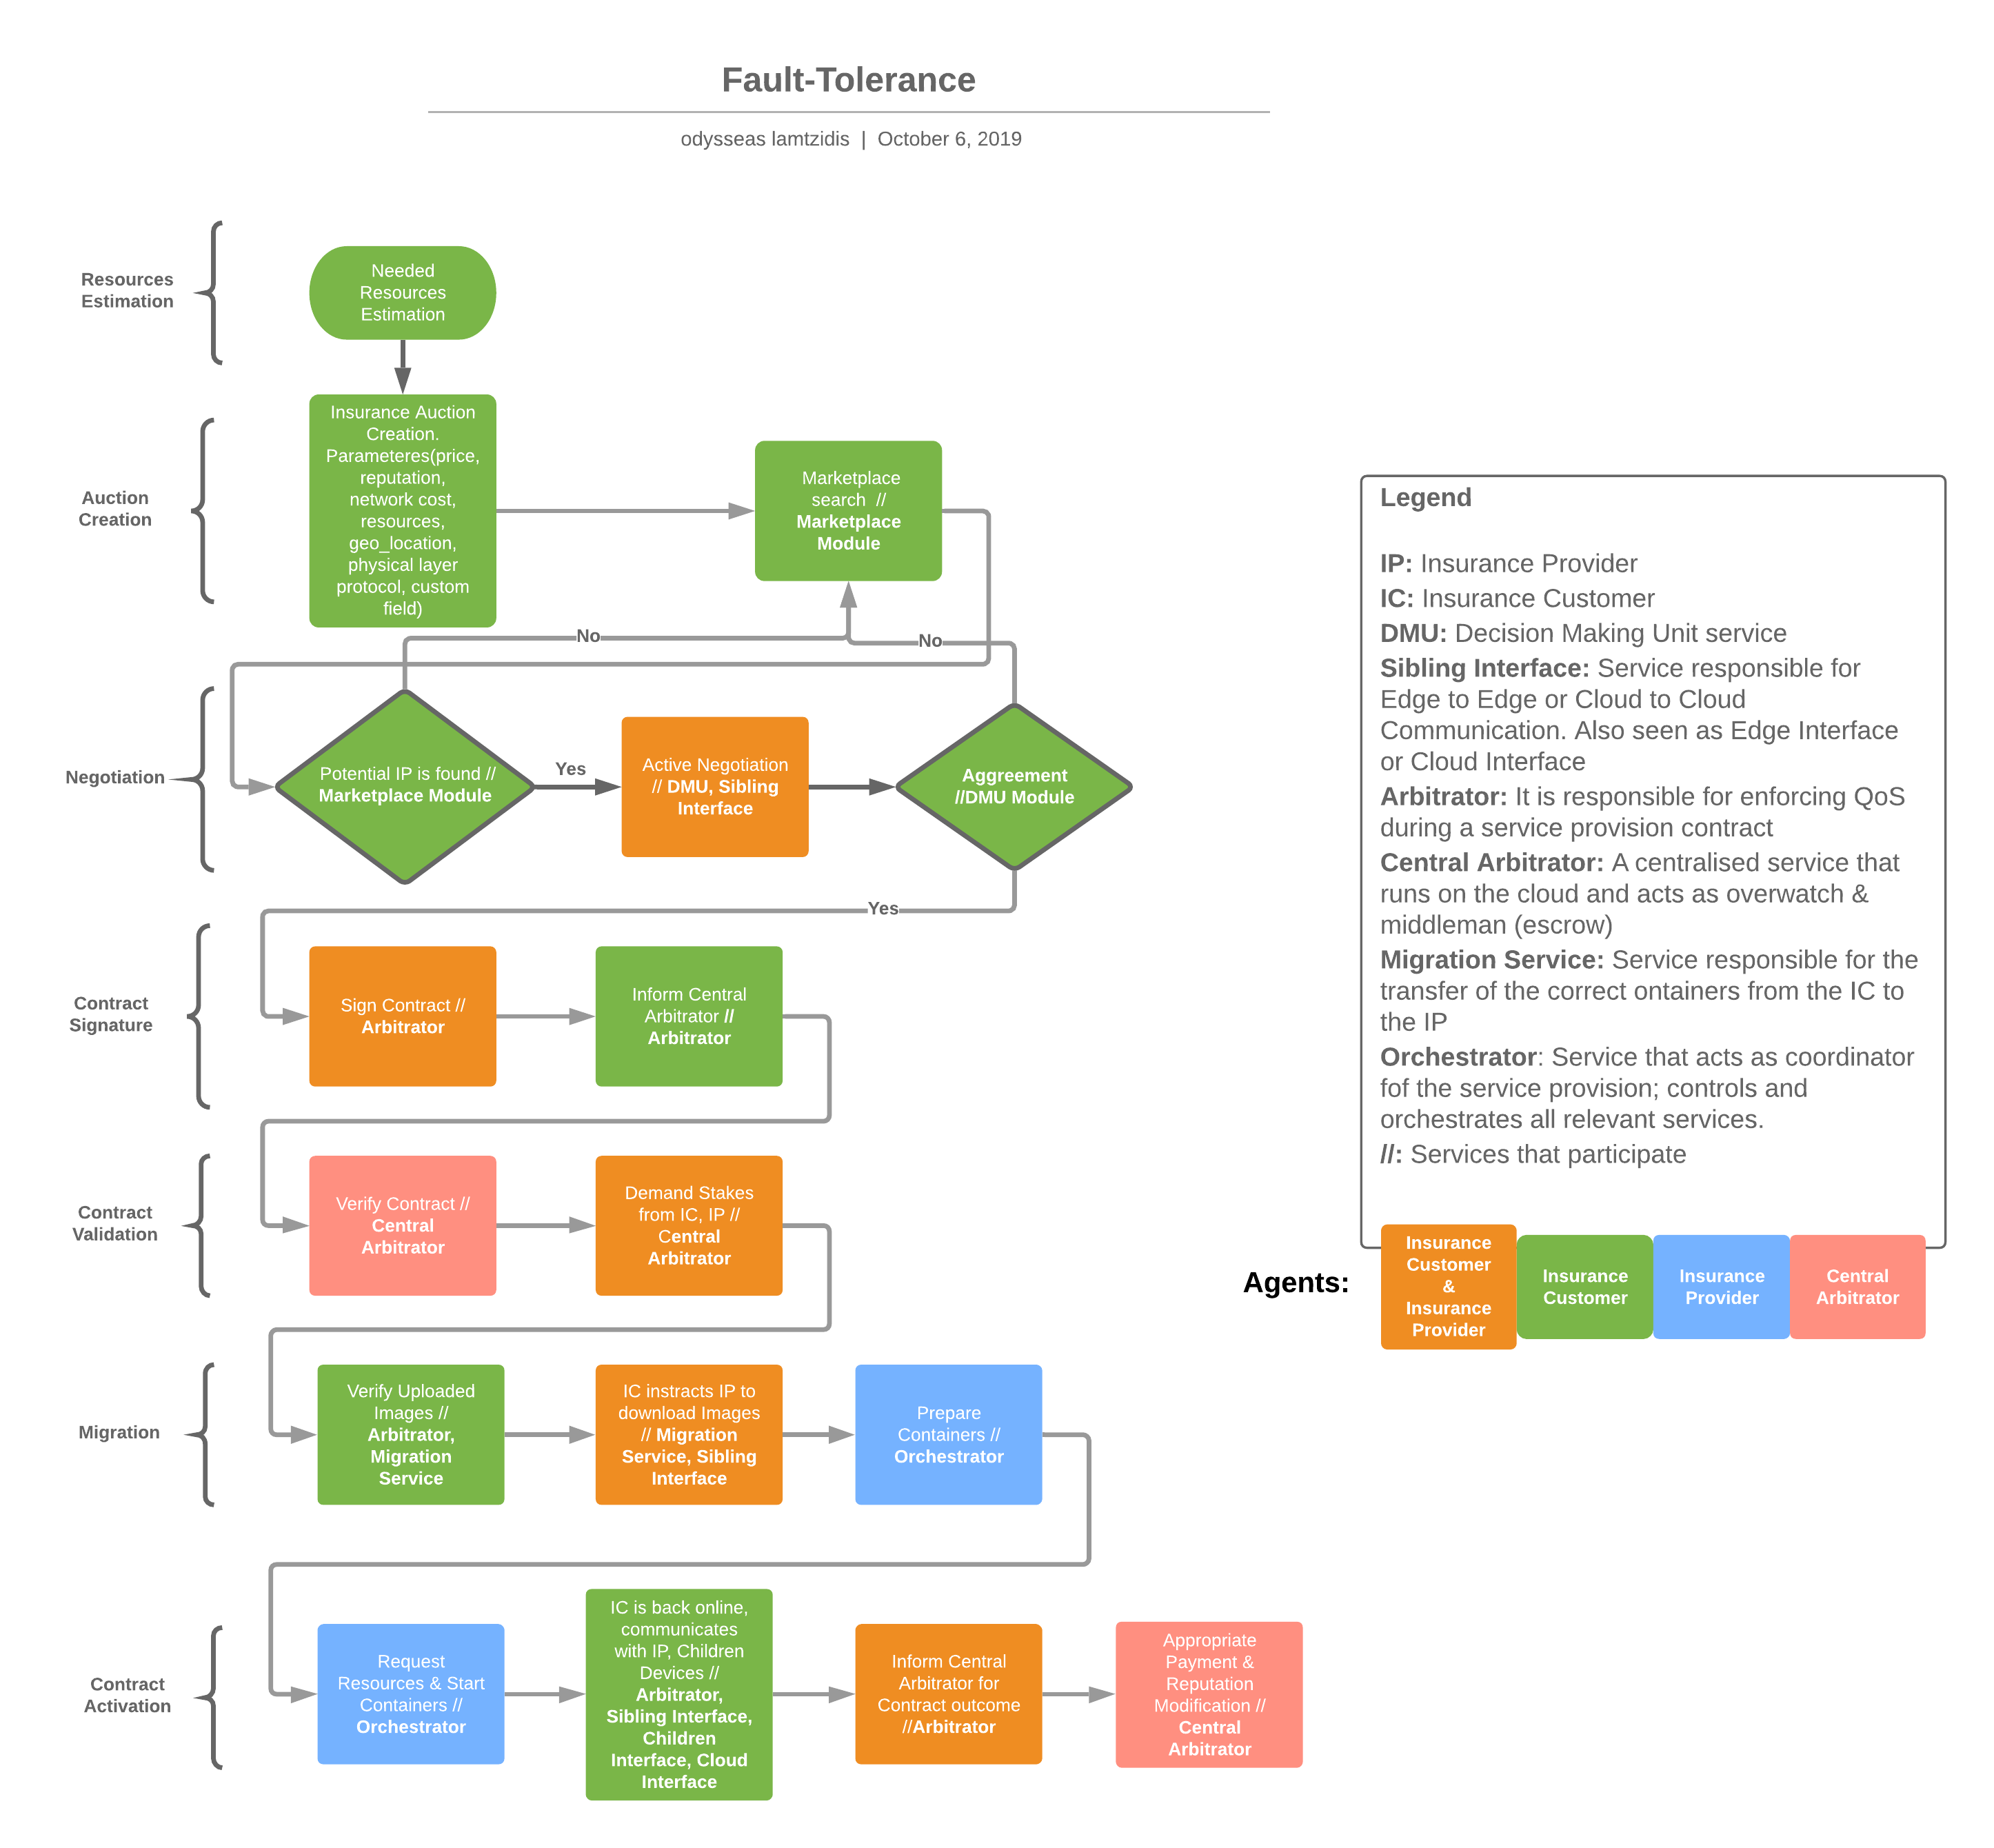
\includegraphics[width=0.8\textwidth]{images/fault_tolerance.png}
    \caption{The Fault-Tolerance reference process}
    \label{fig:fault-tolerance-process}
\end{sidewaysfigure}
\clearpage
\section{Fault-Tolerance High-Level Process at the IoT Edge Layer} \label{st:fault-tolerance}

\subsection{Overview}
In this section we aim to give a gist of the process we envisage for the fault-tolerance scenario, but which can be applied for the more generic \acrfull{eaas} as well. The activity description is not intended as an algorithmic definition, but rather as a high-level presentation of our approach. 

The IoT Edge Node accesses a central marketplace in order to find service-providers. Because of the nature of the fog paradigm, each IoT Edge is interested in systems that are near geographically (from a couple of meters to some kilometres, per the problem domain). Depending on the functionality of the Edge, it is possible that it requires the service-provider to have direct access to it’s sensors (via LoRa, BLE, Zigbee, etc.), which in turn dictates the proximity between the two IoT Edge Nodes. After finding a suitable Edge, the service-provider \acrshort{dmu} service is responsible for handling the negotiation and reaching an agreement.

Let IoT Edge device EdgeA which functions as an insurance customer and has reached an agreement with EdgeB for an insurance contract with certain attributes.
 
Based on the agreement, the service-providers Arbitrator Black Boxes of  EdgeA and EdgeB sign a contract and notify the Central Arbitrator \& the Cloud service-customer Arbitrator. The Arbitrators are responsible for performing \acrfull{qa} on exchange of value/services and perform payment for either honoring or breaching a contract. Since the service, that is being provided in this use-case is an insurance, we will define the service-provider and service-customer as an \textit{insurance-provider} and an \textit{insurance-customer}.

The workflow of an IoT Edge device that requests fault-tolerance services is depicted in Figure \ref{fig:fault-tolerance-process}.
 
By using a hybrid P2P/centralised model, the Arbitrators will be able to reach a consensus in case of breach of contract and perform the needed payment. We assume that the services outlined in the diagram and are shipped as part of the software solution are tamper-proof and thus trusted. They could however exist in a hostile  IoT Edge environment, where additional services actively attack the core package to enforce malicious behavior.  Security audit is out of the scope of this thesis, as we intend to present the notion rather than formally describing it.
 
The handover of the IoT devices from EdgeA to EdgeB is conducted via sending the appropriate containerized services (i.e device services, pre-processing services, etc. ) from EdgeA to EdgeB and then kick-starting those services when the contract is activated.

\textbf{Central Arbitrator:} A centrally run service which verifies the contracts and offers escrow services for payment between stakeholders. It communicates directly with the arbitrator services of both IoT Edge devices \& Back End Nodes.

\textbf{Cloud service-customer Arbitrator:} The arbitrator services of the corresponding Back End service. It performs the same functionality as the IoT Edge Arbitrator.

\subsection{The Marketplace Model}

In the IoT Edge scenario, the problem domain is a location bounded one, since the insurance-provider IoT Edge devices must have connectivity to both the sensors and the insurance-customer IoT Edge device. In contrast with the cloud auction model, this model is consisted of many local markets that function independently but are listed in a single marketplace for enhanced ease of access.
 
At this point, one could argue that probing locally for insurance-providers and using known standard IoT connectivity  protocols, is easier than reaching a central marketplace, finding an appropriate entry and then performing the connection through conventional internet access IPv4/IPv6 (i.e cellular connection, WiFi, Ethernet, etc. ). We believe that this process will be hindered by the inability of most protocols to perform adequately in regards to throughput. While these protocols are optimal for the communication between the sensors and the IoT Edge devices, they are not probably optimal for the Edge to Edge connection.
 
The auction model can be N:1, 1:N or N:M, we choose the latter because it is the most flexible. At any time t1, N IoT Edge devices are able to function as insurance providers and auction their services to potential insurance customers. At the same time, M insurance customers IoT Edges are able to auction a contract for providers to fill.
 
The \acrfull{qos} between the IoT Edges is ensured by the black-box arbitrators which function in good faith since they are considered tamper-proof by the system stakeholder. A centralized service is offered by the \gls{system-provider} to ensure QoS for all the cloud and edge stakeholders. It offers a full-range REST API for IoT Edge to post/update auctions, export statistics or issue custom contracts.
 
The procedure is as follows, (microservices that appear in the architecture as modules are in \textit{italics}). The procedure is organized and orchestrated by the \textit{orchestrator} module that is responsible for the smooth operation.

It consists of phases:
\begin{enumerate}
    \item Resources \& Cost Estimation (Required, Offered)
    \item Auction Creation
    \item Negotiation
    \item Contract Signature
    \item Contract Validation
    \item Migration
    \item Contract Activation
\end{enumerate}

\subsection{Resources and Cost Estimation Phase}

\noindent
\textbf{Insurance Customer:}
The service \textit{Decision Making Unit} (DMU), based on specific and industry state of the art algorithms, in case of customer, performs an estimation of the needed resources. Resources are categorized by industry standard terminology (RAM, CPU, cores, Storage, Bandwidth, Uptime, Network interfaces).

\noindent
\textbf{Insurance Provider:}
At this phase, the \textit{Decision Making Unit} (DMU) of the insurance provider determines the resources (RAM, CPU, Storage, Bandwidth, Uptime, Network interfaces) which will be auctioned in the insurance marketplace.
 
Both Insurance Providers \& Customers formulate an estimation of the preferred value for which they wish to sign the contract based on multiple factors, such as user preference. The final value will be determined in the negotiation phase.

\subsection{Auction Creation phase}
Using the IoT Edge Market REST API, IoT \textit{Edge market interface} issues an auction, detailing the resources needed/offered and other contract details, such as : price, reputation, network cost, geographic location, connectivity layer protocol and other custom fields. During setup phase, the IoT Edge scans for nearby Edges and requests for service-providers by issuing an insurance auction, using common IoT Protocols according to a configuration file (LoRa, BLE, Zigbee, etc.) via \textit{the Edge-to Edge interface}. Moreover, it can scan for IoT Edge devices which are geographically near and communicate using a standard Internet connection, to do this, it uses a centralized IoT Edge Marketplace.

\subsection{Negotiation phase}
After a match is found, the service informs the IoT Edge devices which then continue the negotiation of the offer/demand by using the \textit{DMU} and \textit{IoT Edge Interface}. Web-sockets and a REST API are model protocols for real-time communication. During the negotiation, the IoT Edge devices communicate in order to reach an agreement on the resources and the value that will be staked in the contract. Each IoT Edge can follow it’s own strategy but a reference can be given following a simple rule-based system.

\subsection{Contract Signature phase}
When an agreement has been reached (concerning the contract’s parameters), the IoT Edge \textit{Arbitrators} Black Boxes digitally sign a contract by staking a predetermined amount of value\footnote{Value is arbitrary, can be monetary value, cryptocurrency value, value in services.} and then inform the central Arbitrator of the event. We envisage a mechanism that will be able to perform an irreversible action in order to model the stake of value. A simple idea would be to use already established cryptocurrency projects that support such a functionality (e.g multi-signature addresses).

These microservices are expected to work as tamper-proof black boxes and thus are modeled to be trusted and non-hostile. The \textit{arbitrator} black boxes between IoT Edge devices communicate through the IoT \textit{Edge Interface} and directly with the central Arbitrator. We expect a proper threat model to be presented and a security analysis to be conducted, but we project that the arbitrator will \textit{usually}\footnote{The security analysis and the algorithmical structure of the arbitrator will give as the specification on top of which we will structure the technological stack} function as intended.


\subsection{Contract Validation phase}
The central arbitrator verifies the validity of the signed contract and then proceeds to add it in the active contracts list. The Central Arbitrator demands the stakes from the stakeholders in order to finalize the verification and acts as an escrow for the exchange of value/services.

\subsection{Migration phase}
As presented in Section \ref{st:balena-filecoin}, the IoT Edge stores locally the entirety of application logic, in the form of container images loaded into balenaEngine.

After the contract signature, the Insurance Customer \textit{arbitrator} informs the \textit{migration service} to verify the validity of the system images that are uploaded in the fillecoin DSN and update them as needed. After the verification, the insurance customer’s \textit{migration service} procures the needed keys to the insurance provider’s \textit{migration service} in order to find and download the images from the Filecoin DSN network. The communication with the Filecoin DSN is conducted through the \textit{filecoin interface} service. After download, the \textit{orchestrator} makes all the necessary container setups. 

\subsection{Contract Activation phase}
In case of critical failure, the insurance provider IoT Edge must be informed immediately in order to kick-start the containers and provide the insurance policy in a timely manner. The alert will be given by the insurance customer \textit{arbitrator} if possible or will be detected by the insurance provider.
 
The service provider's \textit{orchestrator} will request resources and spin up the Insurance Customer’s containers. The Service Provider’s \textit{arbitrator} is responsible for ensuring QoS in the insurance-provider  ’s operation according to the signed contract.
 
When the Insurance-customer comes back online, it’s \textit{arbitrator} communicates with the \textit{arbitrator} of the insurance provider, constrained devices and the insurance customer Cloud \textit{Arbitrator} in order to cross reference that operation went smoothly (i.e data analytics performed, data logged \& keys updated, no packet was lost)
 
The service provider's Arbitrator then proceeds to inform the central arbitrator of the certail contract activation, whether the contract was honored or not and finally the central arbitrator performs the appropriate payment and returns the stake to the party that got paid. In this scenario, each stake is the agreed payment, thus if the contract is voided, the insurance provider’s stake is given to the customer and his reputation is reduced or the provider receives the stake of the customer (as payment) and his reputation is increased.



 \clearemptydoublepage
 
  \chapter{Implementation} \label{ch:implementation}
\markboth{Implementation}{}

\paragraph{}

At the core of this thesis, rests the implementation of the above mentioned architecture. In this Chapter, we are going to introduce the protocols and platforms that were used for the implementation, the scenario of the use-case and finally provide a walkthrough of our approach, noting the architecture modules that were actually implemented.

The proposed architecture of Chapter \ref{ch:system-architecture} was implemented with several assumptions, so as to create a proof of concept for a narrow aspect of the design. Moreover, as presented in Chapter \ref{ch:system-architecture}, the architecture is highly affected by the used technologies (i.e EdgeX, Filecoin, etc)

\section{Scenario}

The scenario that was chosen for the implementation of our reference use-case is fairly simple. We assume an edge device that handles a sensor which is connected through LoRa. This edge device has entered into a service contract with another edge device which also supports the LoRa protocol. In our scenario, EdgeA has a failure and EdgeB detects the failure, activates the contract and kickstarts the services in order to control the sensor.

In the implementation, each Edge consists of a Raspberry Pi 3 and a Lorank8 (Beaglebone Black) that are networked over LAN. Although they are two distinct hardware boards, we model our Edge as the combination of those two. Each Edge device has therefore it’s own LoRa gateway, both in terms of software (i.e packet forwarder) and in terms of hardware.


\subsection{Hardware}

For the Edge device, a combination of two hardware edges was used as neither provided adequate performance for our implementation on its own. We started with a Raspberry Pi 3 which would house the entirety of the application logic, while Lorank8 (Beaglebone Black) would only function as the gateway component. After verifying that Raspberry pi 3 was inadequate for the array of microservices that we would run, we opted for a distributed architecture, simulating the Edge device as the networked combination of these 2 boards.

Figure \ref{fig:dist_arch} illustrates the distribution of services between the devices, where each polygon is a distinct microservice. In BalenaOS the microservices are containerized, meaning that each polygon is in essence a single container, while in Debian Jessie, the services run natively on the OS without any form of isolation (increased efficiency).

\begin{figure}[h]
    \centering
    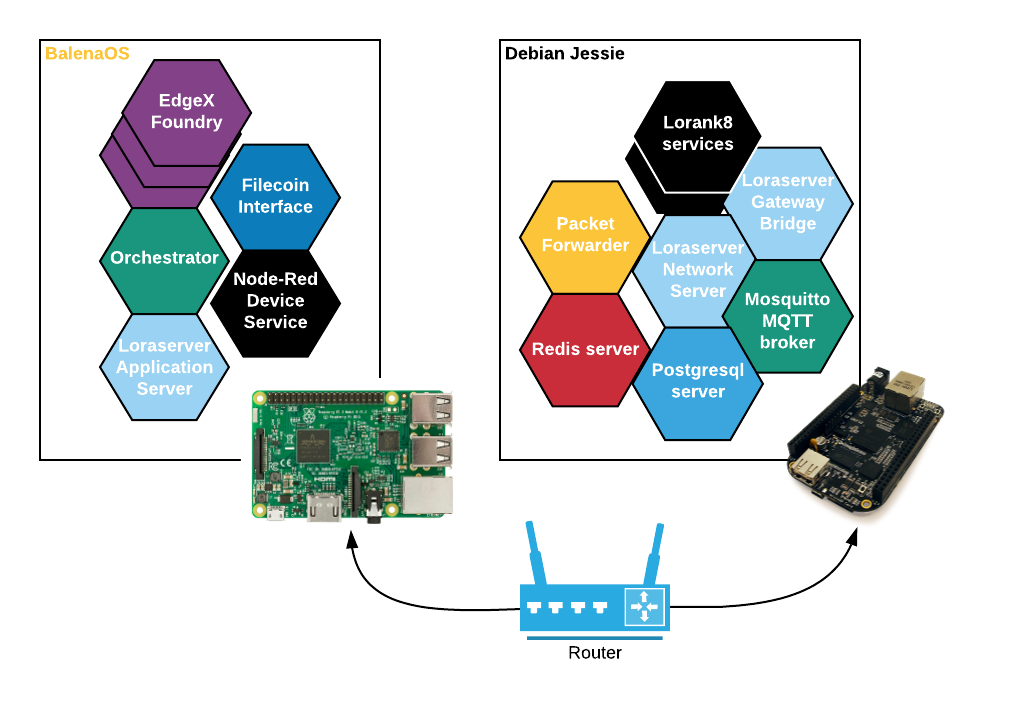
\includegraphics[width=0.9\textwidth]{images/dist_arch_hardware.png}
    \caption{Overview of the distribution of services between the 2 hardware parts of the Edge device}
    \label{fig:dist_arch}
\end{figure}

\subsection{Services}

Moreover, we had to make some assumptions regarding the software and the fault-tolerance mechanism. 

In our scenario it is assumed that the implementation focuses on the handover and not the negotiation process. Thus the marketplace interface, Arbitrator and DMU microservices were removed all-together. Moreover, for matters of efficiency, Filecoin interface and orchestrator were combined in one service, but remain logically decoupled. This means that the two microservices have distinct APIs but are housed in the same program . Finally, the orchestrators of different Edge devices communicate directly, without an Edge2Edge interface intermediary, using HTTP requests and RESTful APIs.

\section{Communication Protocols used in the Implementation}

Before proceeding, we believe it is worth providing an apt description of the communication protocols that are used in the implementation and will be referenced throughout this chapter.

\subsection{MQTT}
\acrfull{mqtt}\cite{mqtt} is one of the most commonly used protocols in the IoT projects and like other internet protocols, it is based on clients and a server. Unlike others, the MQTT makes it easier to implement software and transmit data at a quicker pace, while it also minimizes data packets and consumes less energy. This protocol functions on top of the TCP/IP and it includes a subscriber, a publisher and a broker. The publisher collects the data and sends it to subscribers, using the broker service. It is considerably more power efficient that HTTP.

\subsection{HTTP/REST}
REST, or REpresentational State Transfer, is an architectural style for providing standards between computer systems on the web, making it easier for systems to communicate with each other. REST-compliant systems, often called RESTful systems, are characterized by how they are stateless and separate the concerns of client and server. In the REST architectural style, the implementation of the client and the implementation of the server can be done independently without each knowing about the other (Loosely coupled). Finally, Systems that follow the REST paradigm are stateless, meaning that the server does not need to know anything about what state the client is in and vice versa. When HTTP is used, as is most common, the operations (HTTP methods) available are GET, HEAD, POST, PUT, PATCH, DELETE, CONNECT, OPTIONS and TRACE.

\subsection{gRPC}
gRPC\cite{grpc} is a modern, open source \acrfull{rpc} framework that can run on most computing systems and has clients for most programming languages. It enables client and server applications to communicate transparently, and makes it easier to build connected systems.

Finally, gRPC was firstly developed by Google, uses HTTP/2 as it’s transport-layer protocol and protocol buffers for it’s interface description language. It is also a Cloud Native Computing Foundation (CNCF) project.

\subsection{LoRa}
LoRa (Long Range)\cite{LoRa} is a patented digital wireless data communication IoT technology developed by Cycleo of Grenoble, France. It was acquired by Semtech in 2012, which holds the IP for LoRa transmission methodology. LoRa transmits over license-free sub-gigahertz radio frequency bands like 169 MHz, 433 MHz, 868 MHz (Europe) and 915 MHz (North America). LoRa enables very-long-range transmissions (more than 10 km in rural areas) with low power consumption and low data throughput.
The technology is presented in two parts — LoRa, the physical layer, and; the communication protocol built upon the underlying LoRa physical layer. The communication layer is usually LoRaWAN (Long Range Wide Area Network), an open source communication protocol defined by the LoRa Alliance consortium; Thus, LoRaWAN™ defines the communication protocol and system architecture for the network, while the LoRa® physical layer enables the long-range communication link. LoRa WAN communication protocol ensures reliable communication, secure communication and adds additional headers to the data packets. LoLoRaWAN network architecture is deployed in a star-of-stars topology (vs. mesh topology eg. Zibgee).

The LoRaWAN networks laid out in a star-of-stars topology have base stations relaying the data between the sensor nodes and the network server.
Communication between the sensor nodes and the base stations goes over the wireless channel utilizing the LoRa physical layer, whilst the connection between the gateways and the central server (LoraWAN cloud - network server) is handled over a backbone IP-based network. 

\begin{itemize}
    \item \textbf{Gateways:} At the core of each gateway, runs a packet forwarder\cite{packetfor}. A program that forwards RF packets received by the concentrator to a server (network server) through an IP/UDP link. It also emits RF packets that are sent by the server.
    \item \textbf{Network servers:} They connect to the gateways, de-duplicate data packets (as a packet sent from a sensor might have been picked up by multiple gateways), and then routes them to the relevant application.They can be used for both uplink (i.e. sensor to application) or downlink (i.e. application to sensor) communication. 

\end{itemize}

A reference diagram of a typical LoRaWAN network is shown in figure \ref{fig:LoRa}. In our implementation, we use an open source LoRaWAN project, called loraserver.io.
\clearpage

\begin{figure}[H]
    \centering
    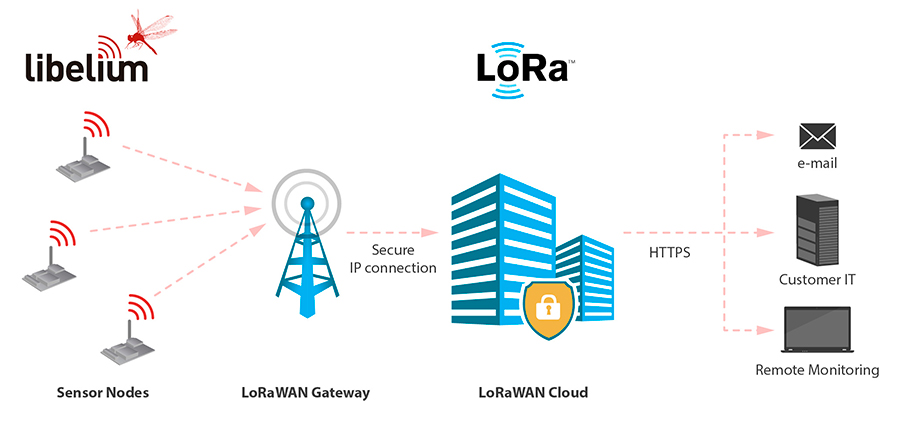
\includegraphics[width=0.9\textwidth]{images/lora_arch.jpg}
    \caption{A LoRa reference architecture, courtesy of Libelium\cite{libelium}}
    \label{fig:LoRa}
\end{figure}

\section{Platforms used in the Implementation}
Having established the communication protocols that are used in the implementation, we now turn our focus on the platforms that were used to develop the implementation. These platforms were not mentioned in the architecture Chapter as they do not consist building blocks of the architecture, but rather choices for our proof of concept. The description of platforms that were presented in Architecture Chapter \ref{ch:system-architecture} will be omitted. Firtly, we believe it’s important to underline the selection criteria for our implementation choices in order to help the reader make informed decisions in case he wants to replicate our implementation.

Criteria, in order of importance:
\begin{enumerate}
    \item Speed of development:  Since we only wish to create a proof of concept for a narrowly defined part of the architecture, the speed of development is our primary drive.
    \item Complexity: Software engineering and robustness of the solutions are out of scope, we used solutions and programming languages that offer the minimum complexity.
\item Performance: We strive to optimise the performance of the chosen solutions due to the restricted nature of the chosen Edge hardware platform.

\end{enumerate}
\noindent
Taking into account the above mentioned criteria, we chose these solutions for our implementation:

\bigskip
\noindent
\textbf{Edge Hardware:} Raspberry pi 3 B+
\newline
\textbf{Edge platform:} Balena
\newline
\textbf{Edge core:} EdgeX Foundry
\newline
\textbf{LoRa Gateway:} Lorank8
\newline
\textbf{LoRa Sensor:} Arduino with Lora/GPS shield
\newline
\textbf{LoRaWAN suite (Gateway, Network-Server, Application Server):} loraserver.io
\newline
\textbf{Software Development:} NodeRed, Python Flask
\newline
\textbf{Development Tools:} Visual Studio Code, Postman, Terminal

\subsection{Raspberry pi 3 B+}

Raspberry pi 3 B+ \cite{rpi3} uses the Broadcom BCM2837B0 system-on-chip (SoC) which includes four high-performance Cortex-A53 (ARMv8) 64-bit processing cores running at 1.4 GHz with 32kB Level 1 and 512kB Level 2 cache memory, a VideoCore IV graphics processor, and is linked to a 1GB LPDDR2 (900 MHz) memory module on the rear of the board. Raspberry pi is in essence a small linux computer and was chosen for the wealth of available software and it’s enormous community, it is considered as the de-facto development \& educational board for IoT Edge linux computers. The board along with it's main components is shown in Figure \ref{fig:Raspberrypi3}.

\begin{figure}[h]
    \centering
    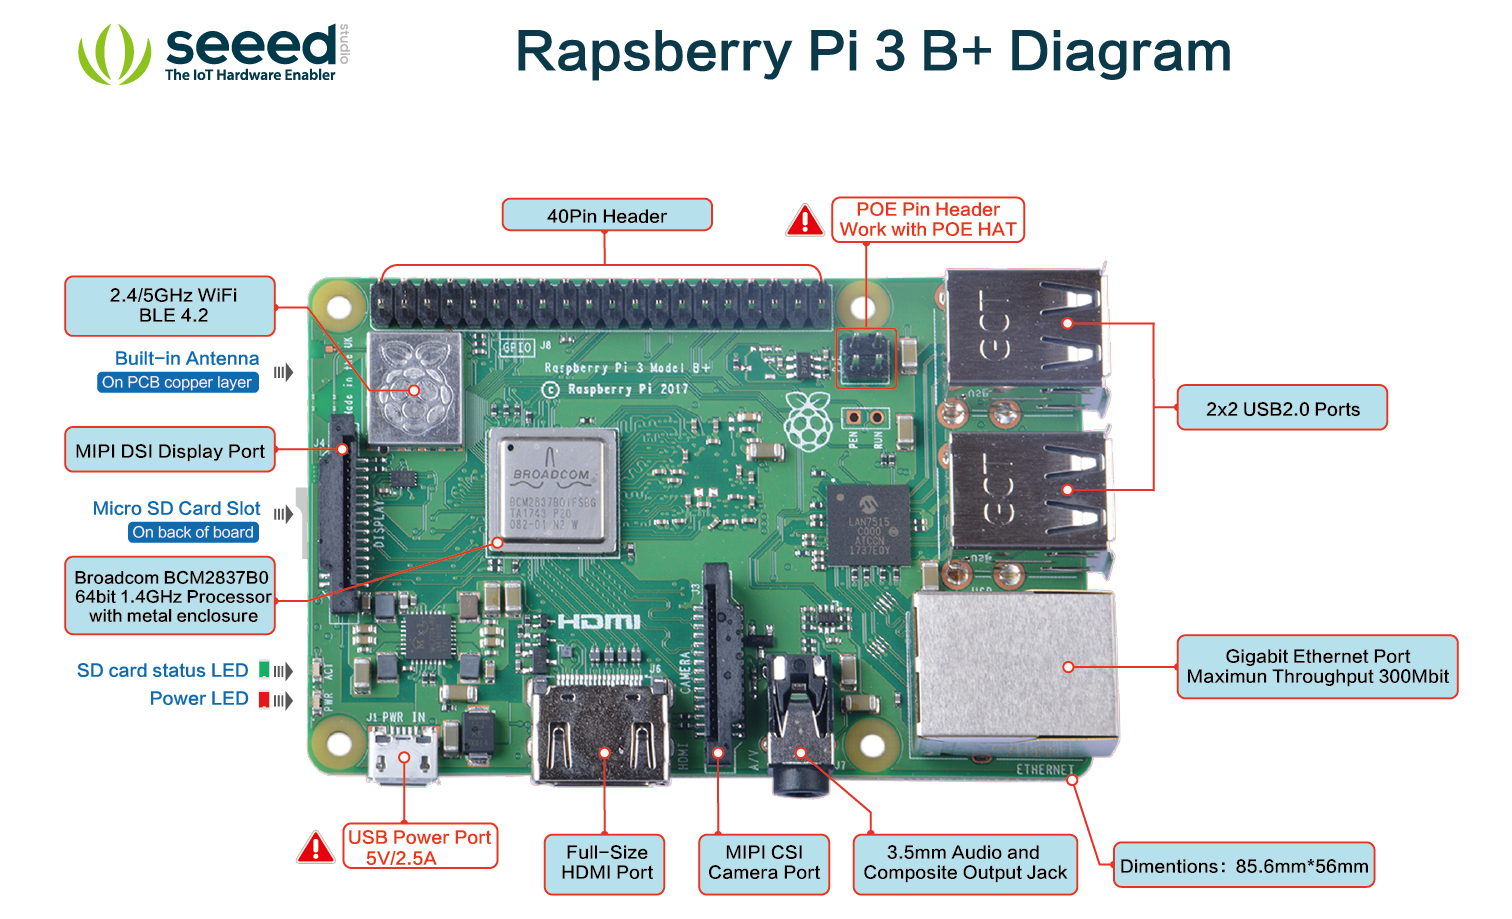
\includegraphics[width=1\textwidth]{images/raspberrypi3.jpg}
    \caption{Raspberry pi 3 B+ and it's components, courtesy of Seeed studio \cite{rpiseeed}}
    \label{fig:Raspberrypi3}
\end{figure}

\subsection{Lorank8}
The Lorank8\cite{lorank8} is a LoRa Gateway with professional specifications. With almost 50 DSP pipes on board it processes 8 LoRa transmissions simultaneously. This enables the connection with several tens of thousands end nodes around the gateway. Moreover, with a sensitivity of -138 dBm and a maximum power of 500 mW it can easily reach the most distant nodes. The hardware is based on the high quality radio board of IMST and the open source Beagle Board\cite{beaglebone}.  The software is open sourced and it works out-of-the-box, enabling us to setup the gateway to our specifications in a short period of time. We opted to enclose Lorank8 in an weather resistant IP67 enclosure, as shown in Figure \ref{fig:Lorank8}.

\begin{figure}[h]
    \centering
    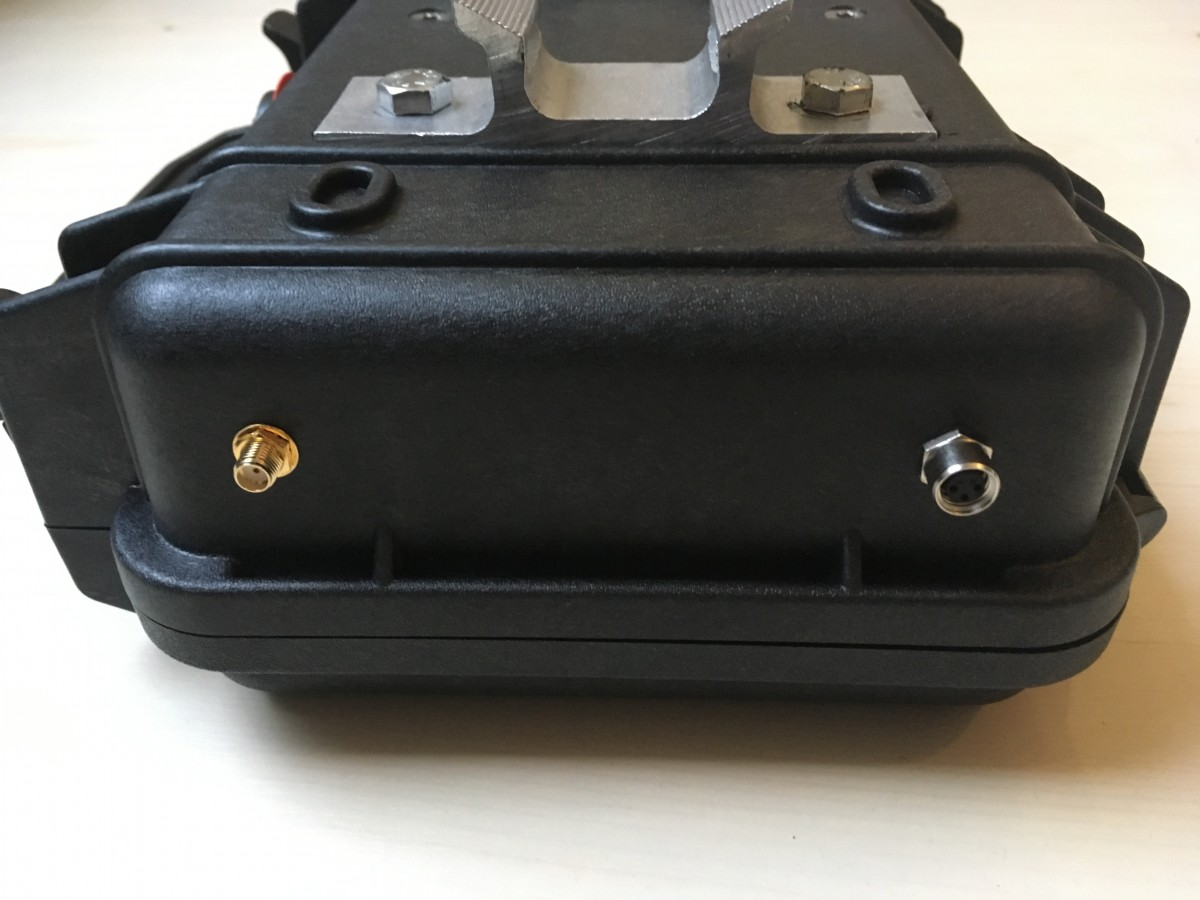
\includegraphics[width=0.5\textwidth]{images/lorank8.jpg}
    \caption{The Lorank8 encased in a weather resistant enclosure \cite{lorank8}}
    \label{fig:Lorank8}
\end{figure}


\subsection{Arduino with LoRa/GPS shield}

Arduino\cite{arduino} is an open source platform that can be used to design various electronic projects. It’s flagship product, Arduino UNO, is based on microcontroller ATmega 328P. It has 14 digital input/output pins (of which 6 can be used as PWM outputs), 6 analog inputs, a 16 MHz quartz crystal, a USB connection, a power jack, an ICSP header and a reset button. It is shown in Figure \ref{fig:Arduino}. Arduino uses its own IDE(Integrated Development Environment),shown in Figure \ref{fig:Arduino_ide}, and is programmed in a simplified version of C++.

The Dragino LoRa/GPS Shield \cite{dragino} is an expansion board for LoRa/GPS for using with the Arduino. It is composed of a LoRa/GPS Shield motherboard and Lora BEE. In the LoRa part, the LoRa/GPS Shield is based on the SX1276/SX1278 transceiver.The transceivers of the LoRa/GPS Shield incorporate the LoRa long range modem that provides ultra-long range spread spectrum communication and high interference immunity whilst minimising current consumption. LoRa also provides significant advantages in both blocking and selectivity over conventional modulation techniques, solving the traditional design compromise between range,interference immunity and energy consumption.

\begin{figure}[H]
    \centering
    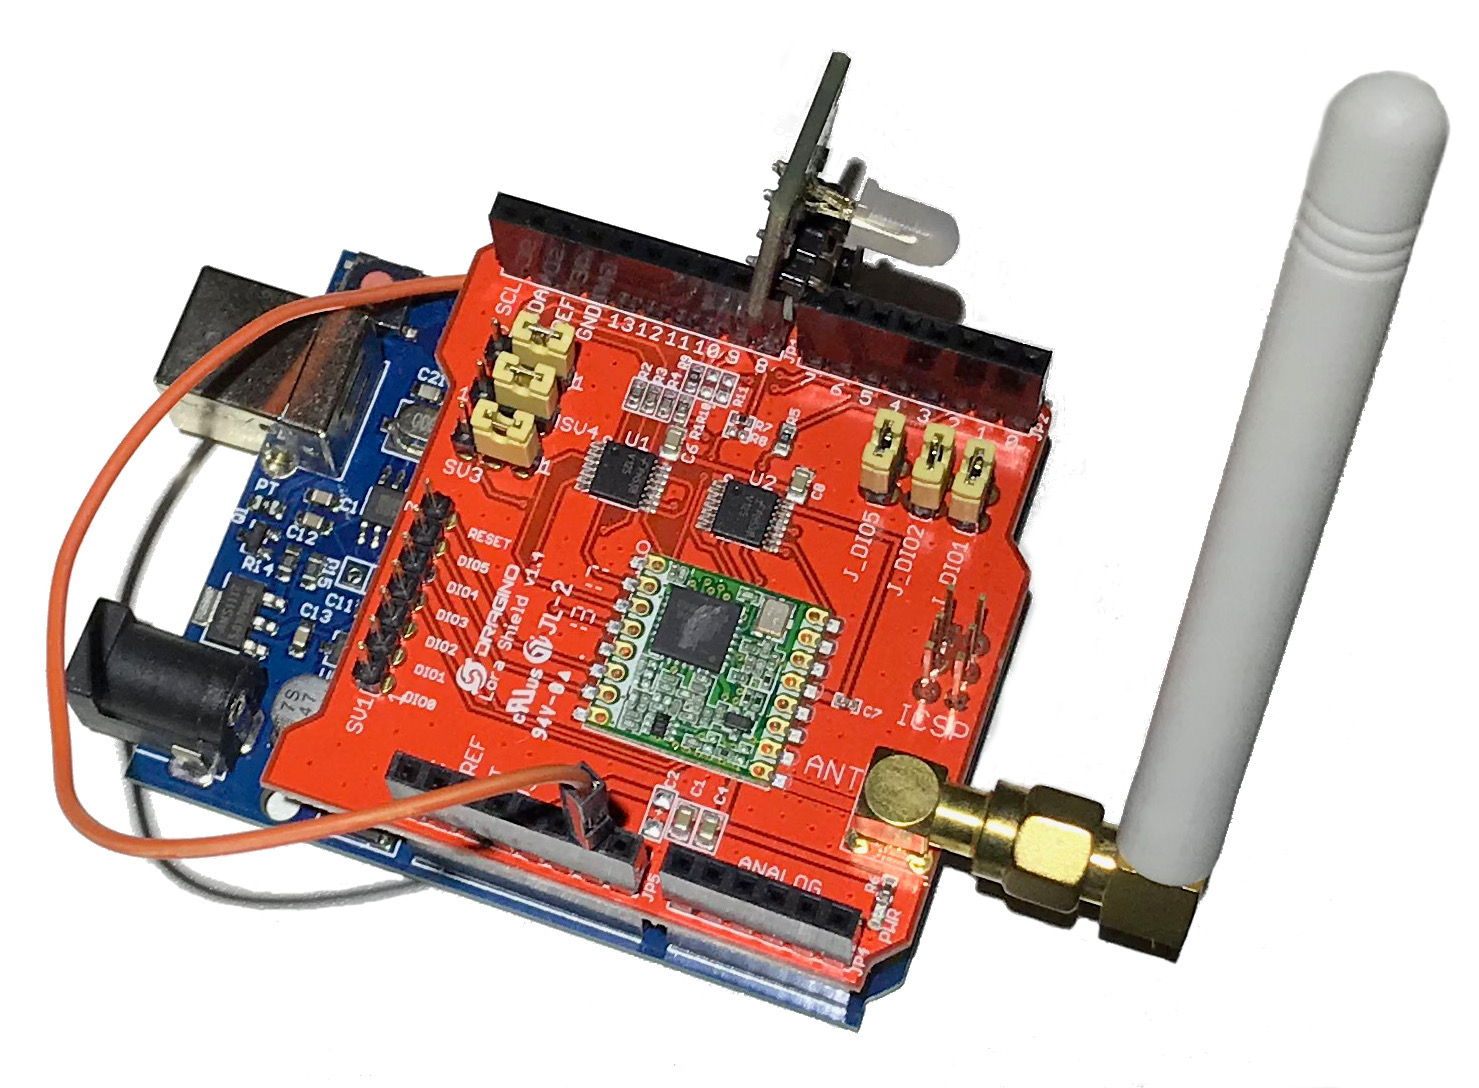
\includegraphics[width=0.4\textwidth]{images/arduino.jpg}
    \caption{an Arduino UNO with the Draggino LoRa/GPS shield \cite{dragino}}
    \label{fig:Arduino}
\end{figure}

\begin{figure}[H]
    \centering
    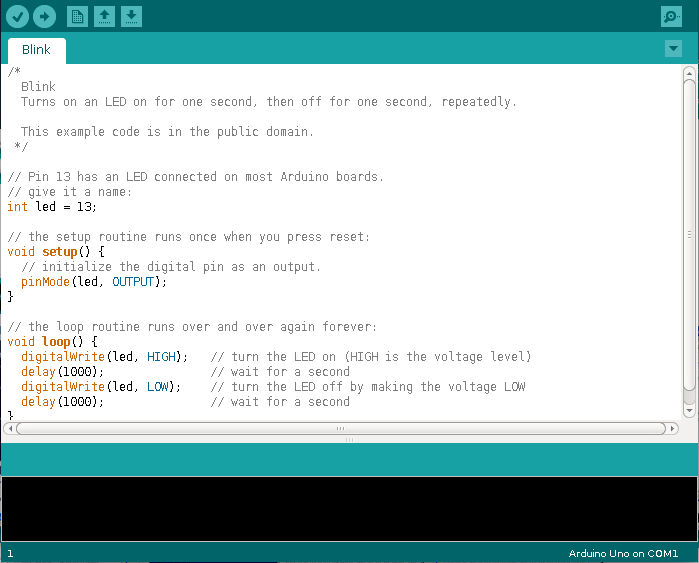
\includegraphics[width=0.5\textwidth]{images/arduino_ide.png}
    \caption{Arduino are easily programmed using the Arduino IDE \cite{arduino}}
    \label{fig:Arduino_ide}
\end{figure}

\subsection{loraserver.io}

The LoRa Server project\cite{loraserver} is an open-source set of applications which is placed between the gateways which receive messages from the nodes to just before the applications receiving the data. It provides mechanisms for managing the gateways on the LoRa network, the applications supported, and the devices associated with the applications.
The project is designed to be used in a very flexible manner and consists of 3 main components:

\begin{itemize}
    \item Gateway Bridge: LoRa Gateway Bridge is a platform which converts the packets outputed by the LoRa packet-forwarder into loraserver.io compatible format (JSON, Protobuf). It receives the UDP packets from the forwarder and outputs an MQTT stream at a connected MQTT broker.
    \item Network server: The network server is responsible for the functionality needed by a network-server (i.e de-duplication of packets, management of the LoRaWAN mac-layer and the handling of uplink/downlink data transmissions).
    \item Application Server: It is responsible for the device inventory, handling join requests and the encryption of application payloads. It offers a web interface and a RESTful and gRPC API.

\end{itemize}
Figure \ref{fig:LoRaserver} illustrates the aforementioned architecture of the LoRaserver project.

\begin{figure}[h]
    \centering
    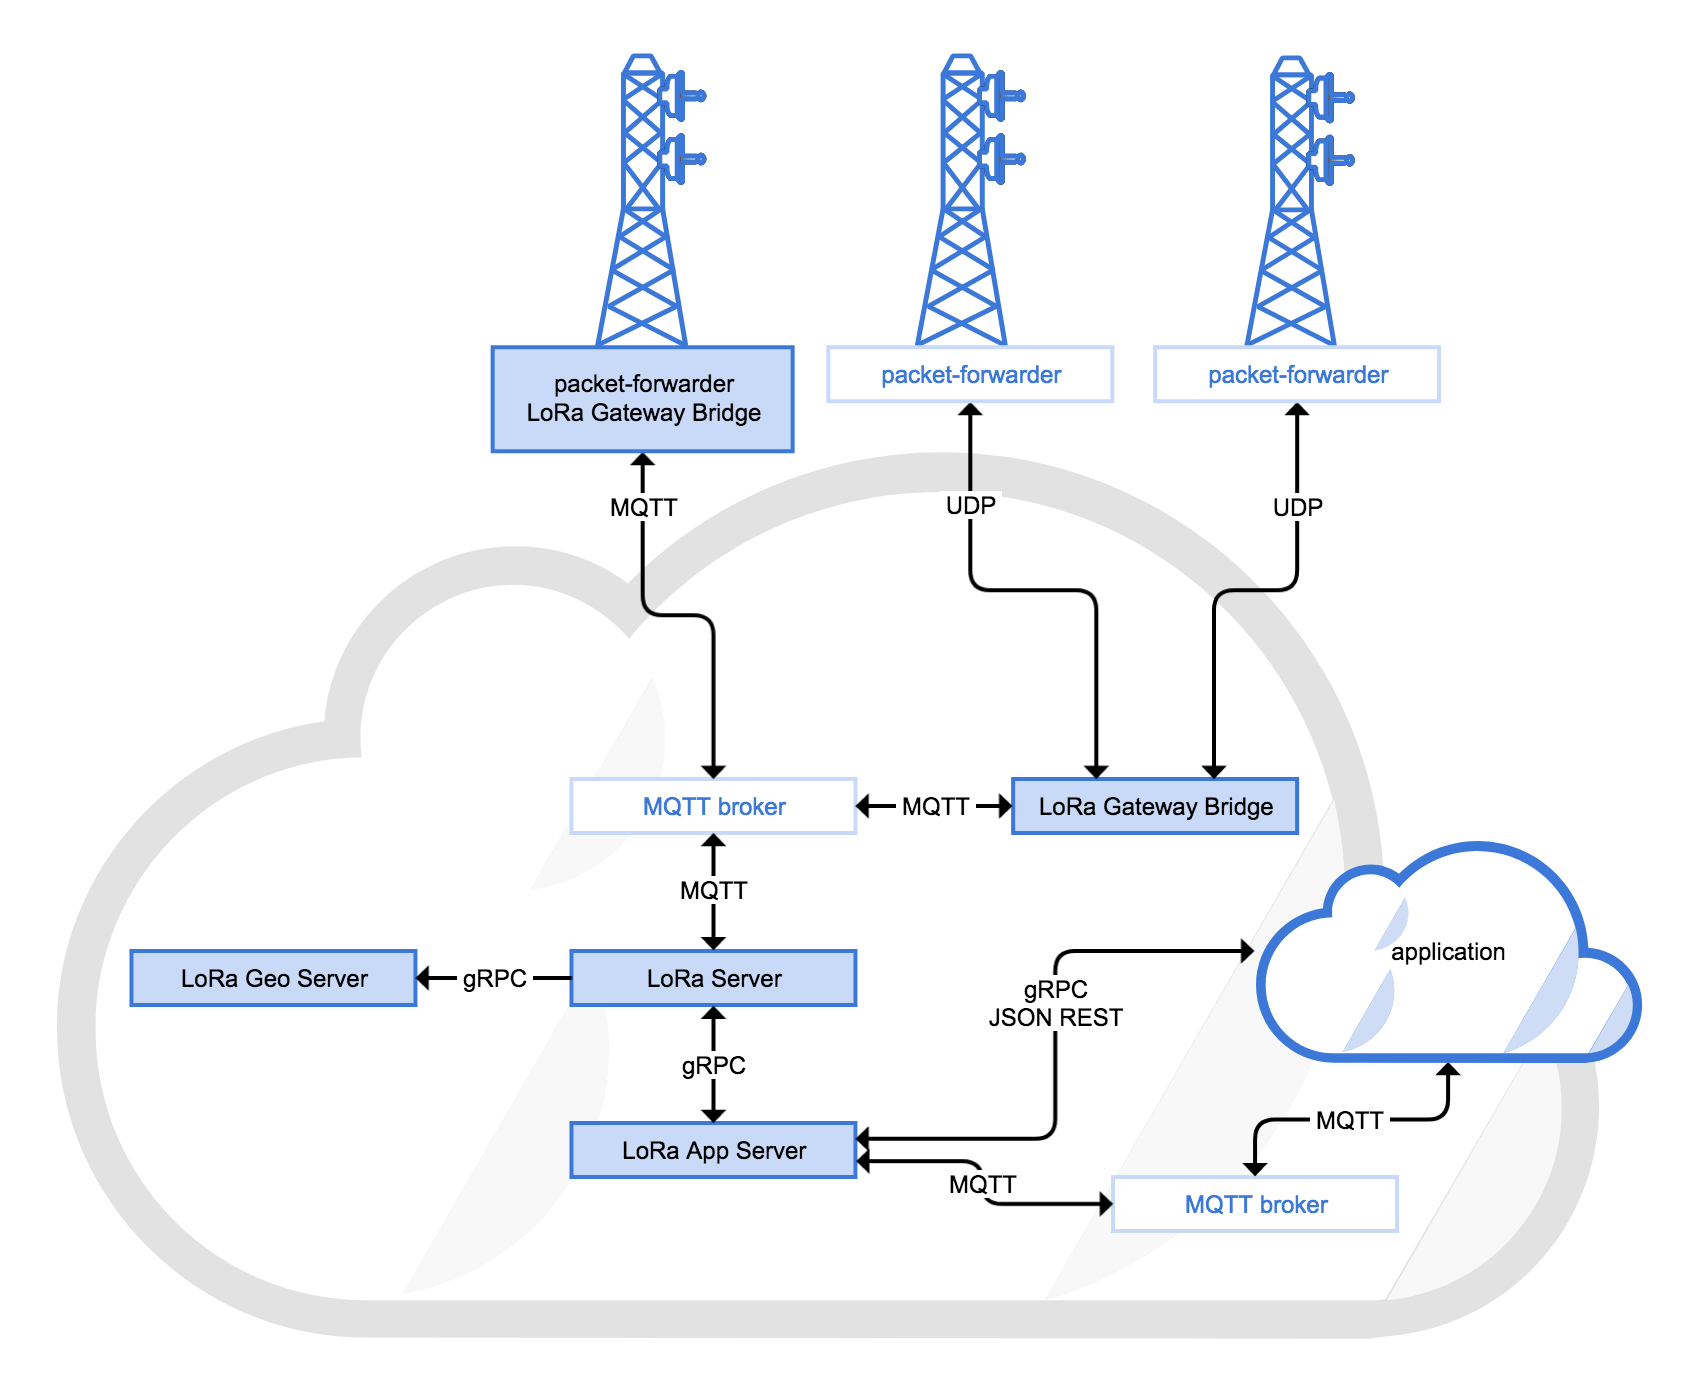
\includegraphics[width=0.8\textwidth]{images/loraserver-arch.png}
    \caption{Overview of the loraserver.io project architecture \cite{loraserver}}
    \label{fig:LoRaserver}
\end{figure}

\subsection{Node-RED}
Node-RED\cite{nodered} is a flow-based programming tool originally developed by IBM’s Emerging Technology Services and is now part of the JS Foundation. Flow-based programming was invented by J. Paul Morrison in the 1970s and is a way of describing an application’s behavior as a network of black-boxes. Each black box has a number of inputs and a number of outputs. It takes the data, performs some abstract computation and then passes the data to the next box.

Node-Red makes programming more accessible to users since it offers the flexibility to create applications, mainly around the IoT domain, without having to worry about a number of common programming hurdles, such as concurrency, execution, etc.  

We used Node-Red to develop various components that could be easily modeled as flows (e.g API resources). Moreover, Node-Red allowed us to focus exclusively on the functionality of the service that was developed. When developing in Node-Red, the developer uses the web GUI to create flows and connect the various nodes. Moreover, it offers customizability by enabling the user to create arbitrary nodes using Javascript. The default data structure that is passed from each node to the next one is named “\textit{msg}” while usually the main input and output component is the attribute “\textit{msg.payload}”. The flows are saved in a json file. An example of a flow is seen in the web GUI  in Figure \ref{fig:nodered}.

On the downside, it’s performance was not adequate for our Edge requirements, since, as of version 0.2.0, it consumes considerable Memory, even for the lightest of functionality. This renders it less favorable versus a python flask script, that has relatively the same learning curve but is considerable more efficient for small scale deployment.

Nevertheless, it’s an ideal tool for proof-of-concepts, due to ease of development, small learning curve and it's immense scalability since it is build on top of a Node.js core.

\begin{figure}[H]
    \centering
    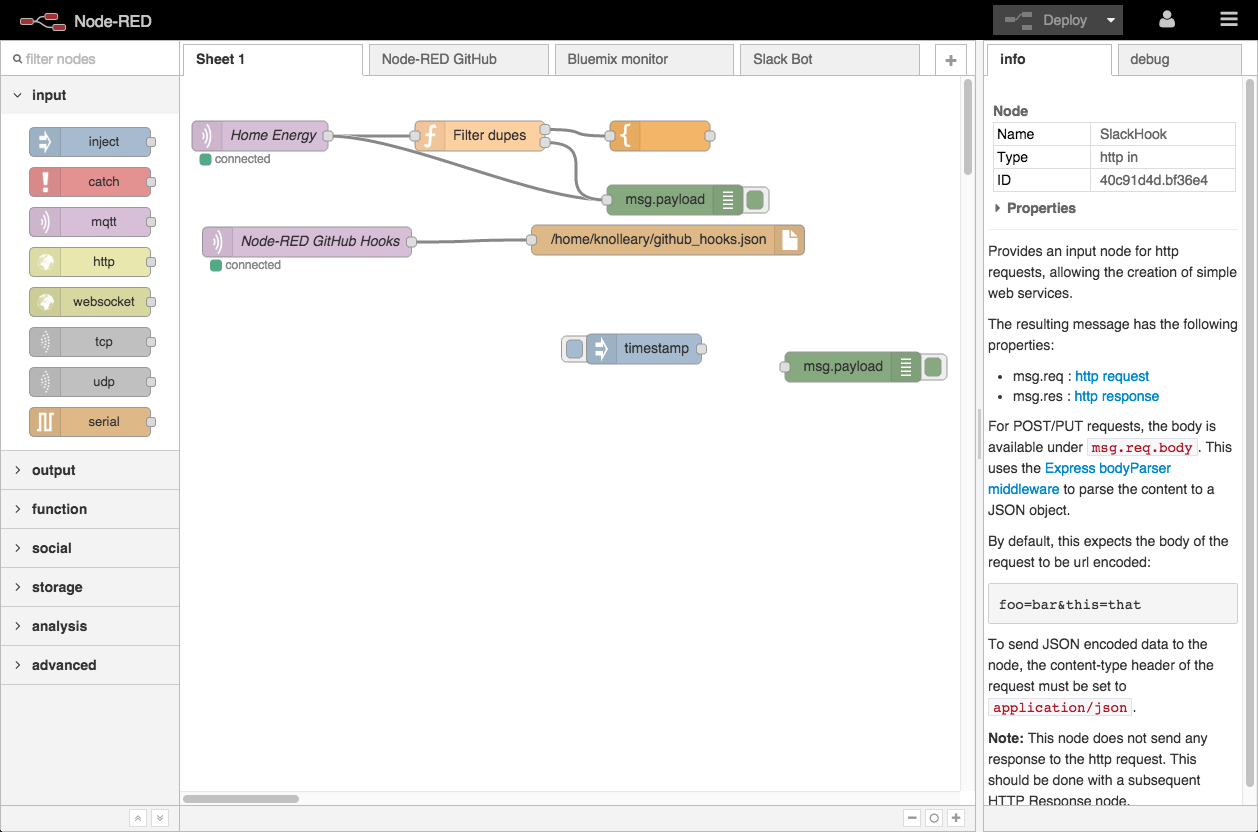
\includegraphics[width=0.8\textwidth]{images/nodered_gui.png}
    \caption{The node-RED web editor GUI \cite{nodered}}
    \label{fig:nodered}
\end{figure}
\newpage

\subsection{Python-Flask framework}

\subsubsection{Python}
Python\cite{python} is a general-purpose programming language that can be used on any modern computer operating system. It can be used for processing text, numbers, images, scientific data and just about anything else you might save on a computer. It is used daily in the operations of the Google search engine, the video-sharing website YouTube, NASA and the New York Stock Exchange.

Python is considered one of the easiest languages to master and understand and is built with ease of use at mind. For that reason, it is mainly used for the speed of development it offers and the small learning curve, while also boasting a huge ecosystem with a wealth of available libraries and frameworks. It is one of the most famous languages to develop the first versions of a product as it is easy to update and change various parts, before converting the stack to a more stable and strictly formatted enterprise solution, such as Java. Python is also the de-facto language used in prototyping and DIY projects, as also for most projects on Raspberry Pi, while it is worth mentioning that lately Node.js and Golang are quickly rising as languages that offer ease of development, namely for web applications (NodeJS) and more generic applications (Golang).

For these reasons, we opted to develop on python a part of the implementation. Since the microservices that we would develop are API based, a web framework was chosen to facilitate us even more. 

\subsubsection{Flask}
Flask\cite{flask} is a lightweight WSGI web application framework. It is designed to make getting started quick and easy, with the ability to scale up to complex applications. It began as a simple wrapper around Werkzeug and Jinja and has become one of the most popular Python web application frameworks. It’s main attribute, is the ease of use, as shown by the “\textit{hello world}” application in Figure \ref{fig:python}. This application shows "Hello, World!" on localhost port 5000 in a web browser when run with the following simple command: \texttt{python app.py}. 

\begin{figure}[H]
    \centering
    \begin{minted}[%
 breaklines,
 mathescape,
 linenos,
 numbersep=5pt,
 frame=single,
 numbersep=5pt,
 xleftmargin=0pt
 ]
{python}
from flask import Flask
app = Flask(__name__)

@app.route('/')
def hello_world():
    return 'Hello, World!'

if __name__ == '__main__':
    app.run()

\end{minted}
    \caption{A flask "hello world" program}
    \label{fig:python}
\end{figure}

\section{Development Tools}
\begin{enumerate}
    \item \textbf{Visual Studio Code:} It is an open-source text-editor\cite{visual} that is easy to use and offers extensive modularity with a wealth of add-ons. It also supports minor IDE-like functionalities, such as debugging, linting, source control, etc. It was used as the main medium to develop the implementation, mainly the python script.
    \item \textbf{Postman:} It is a powerful HTTP client for testing web services\cite{postman}. Postman makes it easy to test, develop and document APIs by allowing users to quickly put together both simple and complex HTTP requests. We used Postman to test EdgeX foundry API as also to test the APIs of the solutions we developed.
\end{enumerate}

\section{Setting up the implementation platforms}
Having established the protocols, platforms and tools that were used to develop this implementation, it is now pertinent to setup the development environment and present a walkthrough on the setup of all the platforms and systems. Afterwards, we will describe the implementation in regards to the architecture, the simplifications that we have made and finally we will talk about the implemented Edge Modules.

The platform was developed on macOS, a unix based system that is akin to Linux and is developed by Apple Inc. The computer is connected to the same LAN as the hardware that was used in the implementation in order to facilitate debugging and deployment. Bash was used as the terminal application of choice and the source code mentioned throughout the implementation is available on github\cite{github-sources}. 
The rest of the implementation walkthrough assume that the implementation replication will be conducted on either a Linux or macOS computer and thus only relevant commands and  software are used. Although Windows replication will not be challenging, the reader will have to research the appropriate tools, software platforms and methods.

\subsection{Balena Setup}

The setup of the balena platform is really simple, as the documents are very explicit\cite{balenaintro}.  Note that when choosing the platform, the user needs to select “Raspberry pi 3 (64 bit OS)”. The Raspberry pi 3 will be featured with the aarch64 version of Balena, still in Beta, as it is needed for the EdgeX to function properly. Aarch64 is the 64bit version of the OS while armv7 (which is default for Raspberry platforms) is 32bit. Thankfully, Raspberry pi 3 supports both OS architecture (but earlier Raspberry pi versions don’t).

The Raspberry should now appear in the application page, shown in Figure \ref{fig:balena_app}. If the user clicks on the device, it will be brought to the dashboard, where the user can overview the services running on the device, the logs the device outputs and also connect to a shell, either to the hostOS, the supervisor container or any user-defined containers. The device view is shown in Figure \ref{fig:balena_device}. We invite the users to playtest balena in order to get comfortable with the platform before proceeding to the rest of the walkthrough. Please note that the “git” related commands shown in the official balena documents, while still functional, are being slowly replaced by balena CLI\cite{balenacli} which is available for both Windows, macOS and Linux.
\newpage
\begin{figure}[H]
    \centering
    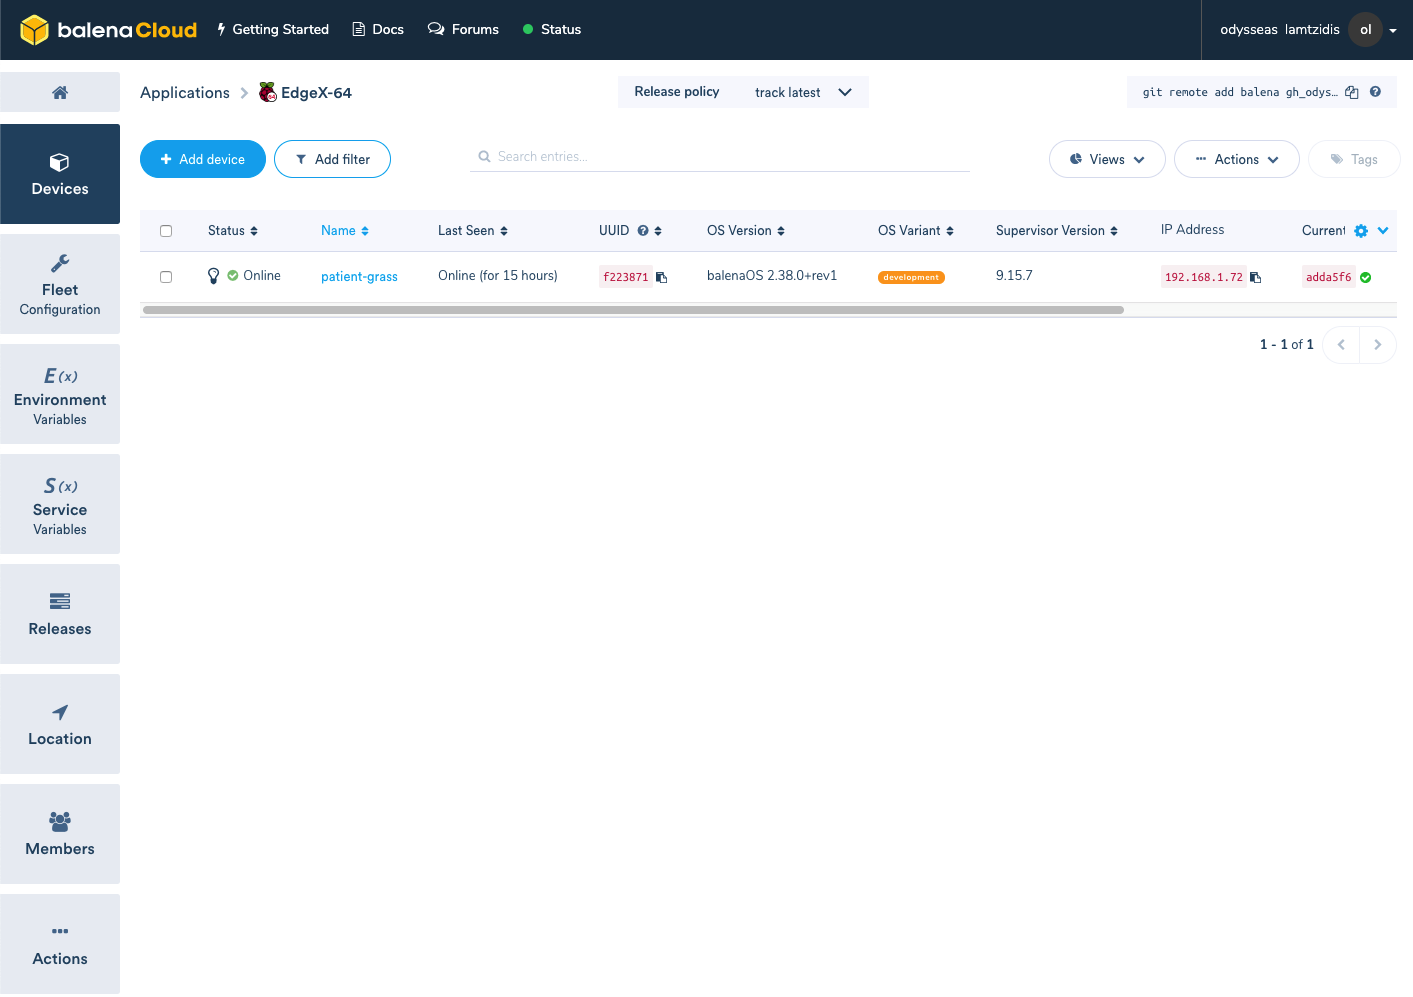
\includegraphics[width=0.9\textwidth]{images/balena_apps.png}
    \caption{Balena Dashboard: The application view where all the devices that belong to the application are shown}
    \label{fig:balena_app}
\end{figure}\begin{figure}[H]
    \centering
    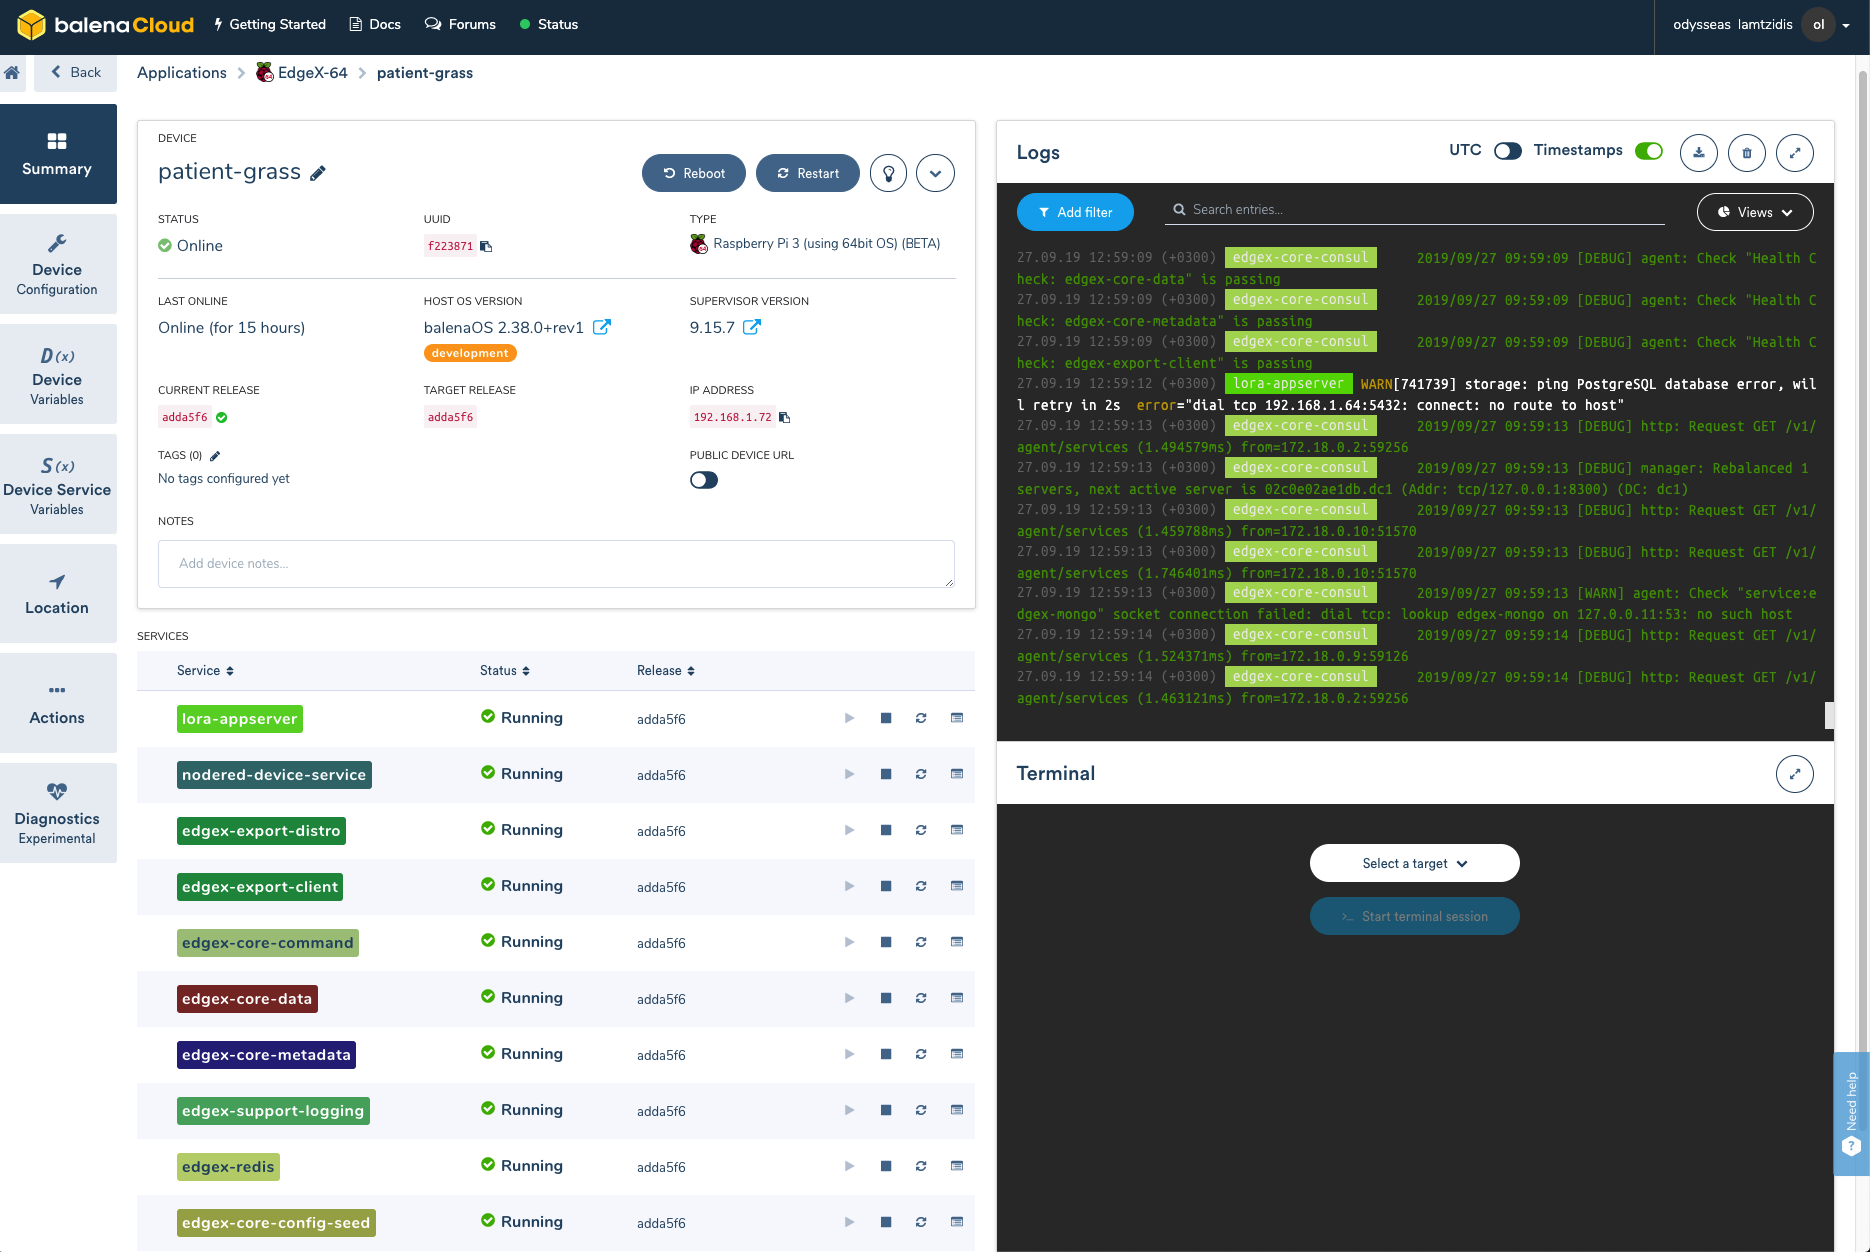
\includegraphics[width=0.9\textwidth]{images/balena_device.png}
    \caption{Balena Dashboard: The device view where device-specific information is shown}
    \label{fig:balena_device}
\end{figure}

In balena, devices belong to a certain application, thus each device added to that application will be installed with exactly the same software. Applications are described as a set of containers (1 to n distinct containers) and their relationship and installation are described by docker-compose version 2.1. In practice, balenaEngine supports a subset of the available docker-compose syntax and functionality, while at the same time enriches it with custom fields, relevant to the balena use-case, such as whether the container should have hardware access. 

\subsection{EdgeX Setup}

Having installed balena, the user now needs to populate the device with services. In order to install EdgeX to balena, the user needs to navigate to the developer-scripts repository of the EdgeX organisation at Github\cite{edgex-github} and find the proper docker-compose that is built for the intended architecture (aarch64-ARM64).

The user might observe that the images dictated in the docker-compose do not mention a specific architecture in their name. This is due to the fact that docker.hub, the image registry from where these images are pulled from, supports images with multiple architectures. Depending on the architecture on which the docker engine runs, docker engine is able to request the correct image from the registry, thus this part is abstracted from the developer.

The version that we integrated into the implementation is 1.0.1 “Edinburgh” which is in fact the first release of EdgeX Foundry. We opted to use the EdgeX docker-compose flavour that supports the Redis\cite{redis} in-memory datastore as storage solution, instead of the Mongo database. This is important for performance issues, as Mongo\cite{mongo} memory requirements rendered the Raspberry pi unusable.

Redis is an extremely efficient in-memory database, which periodically creates a file backup in order to save the state in case of an unexpected shutdown. At this point, it’s important to note that such a solution is sub-optimal for Edge Nodes that need to store the aggregated data over long periods of time, as the data-store’s footprint on the memory will grow substantially. As such, a periodic reset of the data-store is needed; this could be time-based (e.g everyday, at 12:00am) or event-based (e.g if data is pushed to the Filecoin network, then delete).

Regarding our EdgeX installation, we opted to install only a subset of the available EdgeX Foundry services in order to keep the platform’s memory footprint as minimal as possible without sacrificing any of the needed functionality. We proceed to define these services into the docker-compose, following the structure as it is defined in the Edinburgh release docker-compose.

\bigskip
\noindent
\textbf{Installed EdgeX modules:}
\textit{\begin{itemize}
    \item volume
    \item edgex-core-consul
    \item edgex-core-data
    \item edgex-core-metadata
    \item edgex-core-config-seed
    \item edgex-core-command
    \item edgex-Redis
    \item edgex-support-logging
\end{itemize}
}
The final version of the docker-compose can be found at the balena folder of the repository. We note that , in order to remove unnecessary complexity, we have changed the name of the services and removed any networking setting, enforcing thus the services to communicate over the default Docker bridge.

The change of the name of the services is due to the fact that EdgeX services are hard-coded to communicate using the host-names, indicated in the official docker-compose, thus we are enforced to change the services name to the original host-names so they are discoverable one from another. At this point, it is apparent to the reader that containers over the same bridge can communicate using either the container names as host-names or by enforcing another host-name through the appropriate attribute in the docker-compose.

\subsection{Installing EdgeX on Raspberry pi using balena}
To install EdgeX, the user needs to open terminal and:
\begin{enumerate}
    \item \texttt{cd} into working directory
    \item run \texttt{sudo balena login}
    \item run \texttt{sudo balena push <application name>} \textit{\#application name was give during the application creation in previous steps}

\end{enumerate}
The source files will be uploaded into balena servers to build the images, either building them from the source as specified in a Dockerfile, or pulling them from a registry. The EdgeX application will be shipped as soon as the build is ready. The supervisor will then proceed to download the application, pause any running containers and perform the install of updated and new containers and the removal of containers that are no longer defined in the docker-compose file. Finally, the supervisor kick-starts the services according to the dependencies that are also defined in the docker-compose.

\bigskip
\noindent
\subsubsection{EdgeX Walkthrough}
The key aspect the user needs to get acquainted with in EdgeX is the API resources of each microservice, especially if the user intends to integrate other services to the EdgeX Foundry platform. The user is advised to follow the EdgeX API walkthrough tutorial that can be found in the EdgeX documents\cite{edgex-api}, as also review the API docs for each microservice. In this process and for debugging purposes, the use of Postman is advised, as it greatly facilitates it. On top of that, EdgeX offers a set of API tests that can be imported to Postman and function as templates for further experimentation; they can be found in the \textit{developer scripts} Github Repository mentioned earlier.

\subsection{Filecoin setup}

\subsubsection{Client (Storage Consumer) setup} \label{sub:filecoin-client-setup}

In order to interact with the Filecoin network, a user needs to setup a Filecoin Node by following the in-depth walkthrough tutorial \cite{filecoin-walkthrough}.

Filecoin currently is available only for linux and macOS as it is still in alpha version, demanding at the same time, considerable computer resources to run efficiently as the various components are still in development and little optimisation has been made. It is recommended to have at-least a 4 core x86 modern processor and 8GB of RAM, moreover the user should expect to leave the computern running for an extended period of time (in order to synchronise with the network), so the use of a cloud Linux server would be ideal. 

Finally, note that as the go-Filecoin daemon will run in the foreground, it will block the terminal session (or ssh), continuously outputting logging information from the Filecoin node, as shown in Figure \ref{fig:filecoin_terminal}. For this reason, the use of the \texttt{screen} application is advised. \texttt{screen} enables to create virtual terminal sessions from which you can attach and detach, all from one actual terminal session. When detached, the virtual sessions continue to function normally and when attached again, the user can inspect the session history.

\begin{figure}[h]
    \centering
    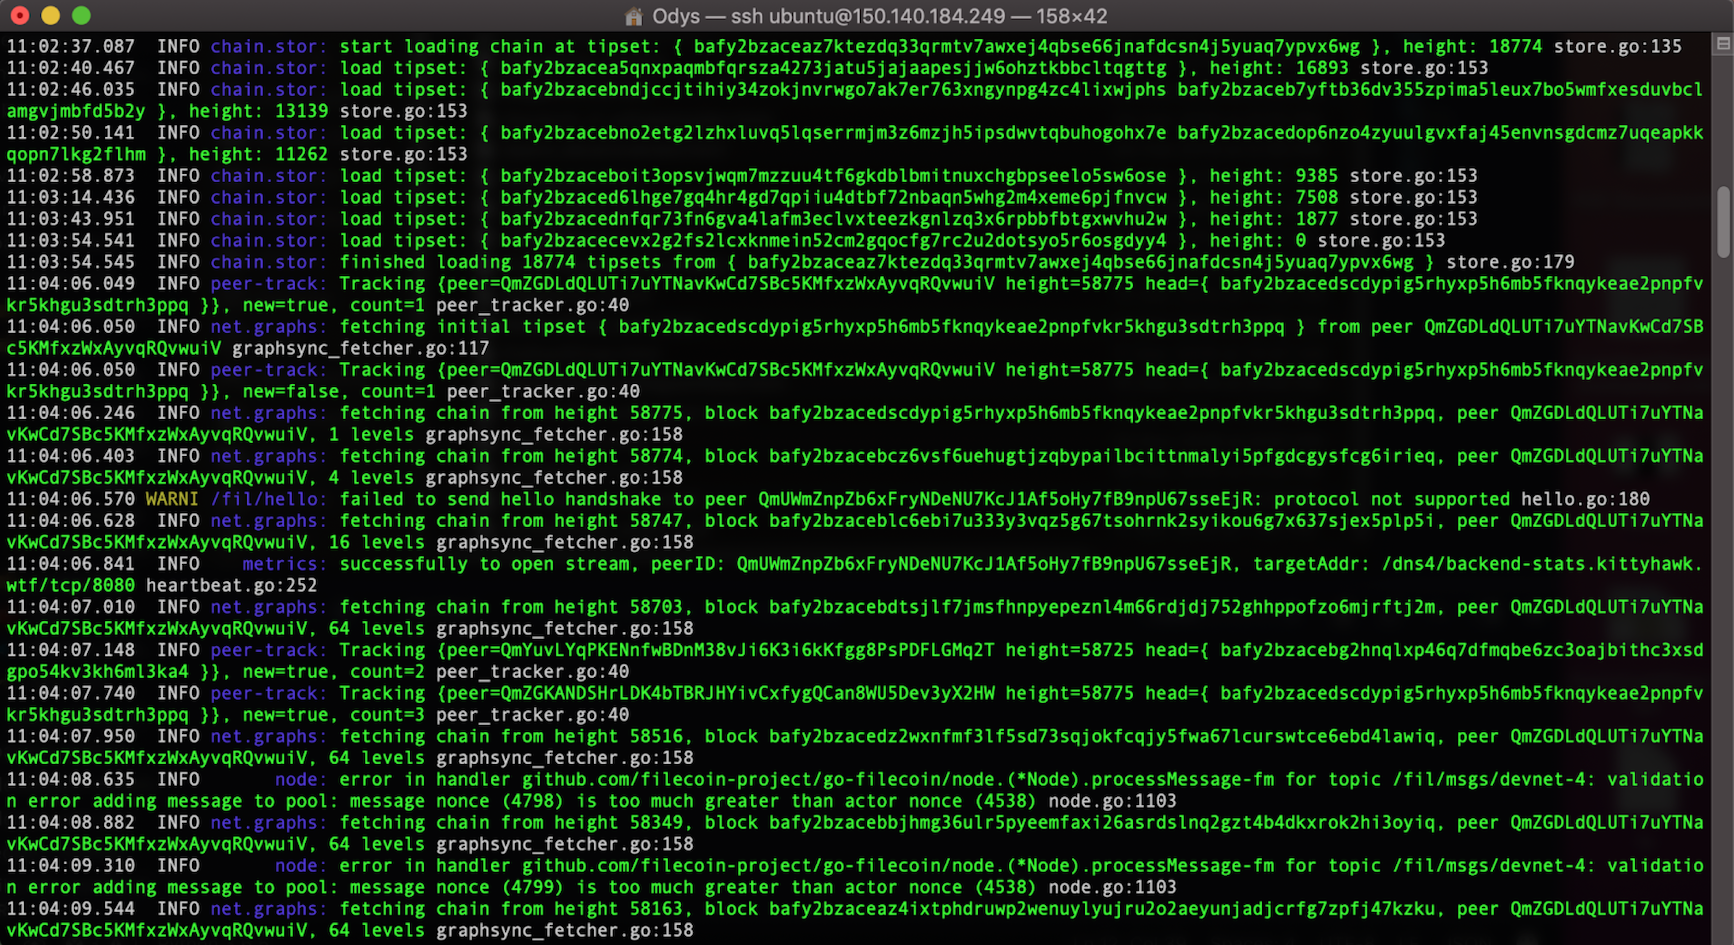
\includegraphics[width=1\textwidth]{images/filecoin_terminal.png}
    \caption{A terminal window outputting STDOUT from go-filecoin daemon}
    \label{fig:filecoin_terminal}
\end{figure}

In order to use the Filecoin network as storage client, the user needs to use the Filecoin faucet and fill the node’s wallet address with Devnet FIL, as outlines in the already referenced walkthrough tutorial.

\subsubsection{Miner (Storage Provider) setup}

In the Filecoin docs, the user can also learn about setting up a filecoin node for mining. We remind the reader that in the Filecoin network, the blockchain miner is the storage provider and mining power is a function of the provided storage and the available storage in the network. When mining, the storage provider gains FIL by providing storage (ask orders) and by verifying and sustaining the integrity and correctness of the blockchain.


\subsubsection{Notes}
We find enlightening to further expand on some parts of the walkthrough.
\begin{enumerate}
    \item \textit{Commit storage?} In the current Filecoin implementation, the miner does not commit a specific amount of storage, but rather it is committed in an ad-hoc basis. The miner sets the price and it automatically accepts any deal from any client.
    \item \textit{Price?} The listed price is in FIL/byte/block. In the blockchain, a new block is mined roughly every 30s, thus in a day (24 hours * 60 minutes * 60 seconds) 2880 new blocks are mined. If the miner wants the price to be valid for a day, he will set a limit of 2880 blocks. Conversely, if a client wants to store 1 byte for 1 day and the price is 1 FIL, then he will pay to the storage provider 2880 FIL.
    \item \textit{gas?} The gas is a term popularised in the ethereum ecosystem. In essence, each time a block is mined, the block miner(s) earn not only the reward in that block, but also the gas given by all the nodes whose transactions are encapsulated into that block. The higher the gas value, the more “valuable” the transaction will be for the prospecting miners, thus it will have a higher priority to be put into the next block over other transactions. (faster confirmation rate).
\end{enumerate}

\section{Lorank8 setup}
Lorank comes pre-installed with certain software but the user will need to enrich it for this implementation. An in-detail guide of how to Quick start with the Lorank8 can be found on Github\cite{Lorank8-manual}, maintained by the company that manufactures and sells Lorank8 itself. A thorough reading of the document is prerequisite to understand the device and start the custom configuration. After following the steps dictated in the Quick Start section of the manual, the user can proceed in configuring the gateway.

\subsection{Configure ssh and install software in Lorank8}
Before continuing, it’s time to introduce an elementary (though highly important) piece of software. SSH, also known as Secure Shell or Secure Socket Shell, is a network protocol that gives users, particularly system administrators, a secure way to access a computer over an unsecured network. SSH also refers to the suite of utilities that implement the SSH protocol. Secure Shell provides strong authentication and encrypted data communications between two computers connected over an open network such as the internet.

In order to ssh into Lorank, the user can either use the local hostname of the device, leveraging the local avahi software that exists or the local IP. In order to connect by using a local IP, we used the program \textit{lanscan} to search for all the devices that exist in the local network and then find the device with hostname “Lorank8”. To use avahi, we simply use “Lorank8.local” in place of the IP. The .local suffix tells avahi to search the network for a device with hostname “Lorank8”.

Now that there is an open ssh connection with Lorank8, it’s time to install the software that will be used (e.g loraserver.io suite). The following commands are executed in order to update the system and install the required software.

\begin{minted}[%
 breaklines,
 mathescape,
 linenos,
 numbersep=5pt,
 frame=single,
 numbersep=5pt,
 xleftmargin=0pt
 ]{bash}
apt-get install update 
apt-get upgrade
apt-get install screen #the same program mentioned in Subsection $\ref{sub:filecoin-client-setup}$
apt-get install htop #a visual upgrade of the top command, used for debugging.
\end{minted}
Then, we proceed to install a MQTT broker (mosquitto), add the LoRaserver repository to the repository lists of the device and install LoRaserver gateway bridge and LoRaserver network server.

\begin{minted}[%
 breaklines,
 mathescape,
 linenos,
 numbersep=5pt,
 frame=single,
 numbersep=5pt,
 xleftmargin=0pt
 ]{bash}
apt-get install mosquitto
sudo apt-key adv --keyserver keyserver.ubuntu.com --recv-keys 1CE2AFD36DBCCA00
sudo echo "deb https://artifacts.loraserver.io/packages/3.x/deb stable main" | \
sudo tee /etc/apt/sources.list.d/LoRaserver.list
sudo apt-get update
sudo apt-get install Redis-server
sudo apt-get install LoRa-gateway-bridge
sudo apt-get install LoRa-LoRaserver

\end{minted}

Finally, LoRaserver network-server requires Postgresql\cite{postgresql} to function. This is challenging since the official support of Postgresql for beaglebone (armv7 architecture / debian 8 “Jessie”) is until version 9.4 but LoRaserver requires version 9.5+. Thus, we will have to use the backports version of Postgresql 9.5 stretch debian.

Backports are re-compiled packages from testing (mostly) and unstable (in a few cases only, e.g. security updates) in a stable environment so that they will run without new libraries (whenever it is possible).

Thankfully, some online research came to fruition\cite{backport}, providing the Lorank8 with the appropriate version of Postgresql.

\bigskip
\noindent
\subsubsection{Configuration of Postgresql}
Having installed Postgresql, it is now required to create a database for LoRaserver to use, so we run the following commands:

\begin{minted}[%
 breaklines,
 mathescape,
 linenos,
 numbersep=5pt,
 frame=single,
 numbersep=5pt,
 xleftmargin=0pt
 ]{bash}
sudo -u postgres psql
create role LoRaserver_ns with login password 'dbpassword';

-- create the LoRaserver_ns database
create database LoRaserver_ns with owner LoRaserver_ns;

-- exit the prompt
\q
\end{minted}

\noindent
Finally, if the following command run successfully, the setup is completed.

\begin{minted}[
 breaklines,
 mathescape,
 linenos,
 numbersep=5pt,
 frame=single,
 numbersep=5pt,
 xleftmargin=0pt
 ]{bash}
psql -h localhost -U LoRaserver_ns -W LoRaserver_ns
\end{minted}


\subsection{Lorank8 Configuration}
Having installed the necessery software, it is required to configure the gateway. The working directory is the root directory and the configuration files are available on Github.

Firstly, we configure \textit{global\_conf.json} that can be found in the Lorank8v1 directory, the configuration rests unchanged except for the server output, where we change the default TTN to localhost, \textit{port 1700}. In other words, we instruct the packet forwarder to output the UDP packets to the LoRaserver gateway bridge. We restart Lorank service using the following command: \texttt{systemctl restart Lorank.service}. Finally, the user should note down the gateway ID found in the \textit{local\_conf.json }in the same directory, it will be used later in the implementation.

To configure the gateway bridge and LoRaserver, we create the appropriate \textit{TOML} configuration files in our working directory, as per the LoRaserver documents instructions. We opt to have the configuration in the working directory as we will run the services in foreground using \texttt{screen}, so as to monitor logging information and change configuration in a breeze. Configurations are left to default.

\subsection{Start the Lorank8 gateway services}

After establishing an active \texttt{ssh} connection with Lorank, we run \texttt{htop} to overview the running processes, it is pertinent to close any browser connection to Lorank and kill the \textit{node.js} processes (the web server) as we won’t be using the web interface and it can save considerable resources in respect to cpu and memory.

Moreover, the user needs to ensure that Redis and Postgresql run on the device by running the following commands:

\begin{minted}[%
 breaklines,
 mathescape,
 linenos,
 numbersep=5pt,
 frame=single,
 numbersep=5pt,
 xleftmargin=0pt
 ]{bash}
sudo systemctl start Redis-server
sudo systemctl start Postgresql
\end{minted}

The user then proceeds to start 1) \texttt{LoRaserver} gateway bridge, 2) \texttt{LoRaserver} and 3) \texttt{mosquitto} server on 3 distinct \texttt{screen} sessions, by starting a \texttt{screen} session, then running one of the following commands: \texttt{LoRaserver}, \texttt{LoRaserver-gateway-bridge}, \texttt{mosquitto} and then detaching from the \texttt{screen}. 

It is important to run the commands from the working directory so as they use the configuration that is saved in the same directory, otherwise the processes will use the default ones that can be found in the \texttt{/etc/} directory.

Lorank is now ready to be used with the rest of the implementation. Each packet that the concentrator receives, is forwarded to gateway-bridge which in turn converts it into an MQTT message that is picked by the network-server and finally will be routed to the appropriate application server.

\subsection{Arduino LoRa mote setup}

Regarding the LoRa sensor (mote), it uses \acrfull{abp}, where the Device Address and Session keys are pre-configured (unlike OTAA, where a DevEUI and application key is pre-configured, while the DevAddr and session keys are assigned/generated in the over-the-air-activation procedure). This means that the application server will be able to read any reading coming from a mote that has a the specific network key and application key combination. The implementation would also work with an OTAA device, but we chose ABP for simplicity.

To setup Arduino, we used the default sketch found in the Github of Arduino LMIC \cite{Arduino-lmic} .It’s a project based on the IBM LMIC (LoraMAC-in-C) but modified to run on Arduino. After downloading the sketch and the Arduino IDE, we can flash the sketch in the Arduino and make the proper GPIO connections between the shield and the Arduino as stated in the draggino docs\cite{dragino}. As soon as the Arduino is connected to power( either USB or wall-wart), it will start broadcasting to all gateways in a radius of several kilometers. The payload of the Mote is only decryptable by using the combination of the two keys mentioned before, these keys are only known to our Iot Edge device.

\section{Device Service Component}
The device-services function is to integrate a LoRa device to the EdgeX platform. In essence, the device service can be seen as a platform with a south and north side. The south side connects to the LoRa infrastructure of the edge device (network server) while the north side propagates the data it received from the south to the EdgeX infrastructure. Figure \ref{fig:device_service} illustrates the high level architecture of the device service in a highly simplified diagram that focuses on the device service.

Thus, one component is responsible for managing the LoRa device and LoRa infrastructure and the other is responsible for handling EdgeX. Thus, the node-RED service must:
\begin{enumerate}
    \item Interface with 2 different APIs which implement different specifications and semantics
    \item Expose 2 different APIs that follow different specifications and semantics

\end{enumerate}

\begin{figure}[h]
    \centering
    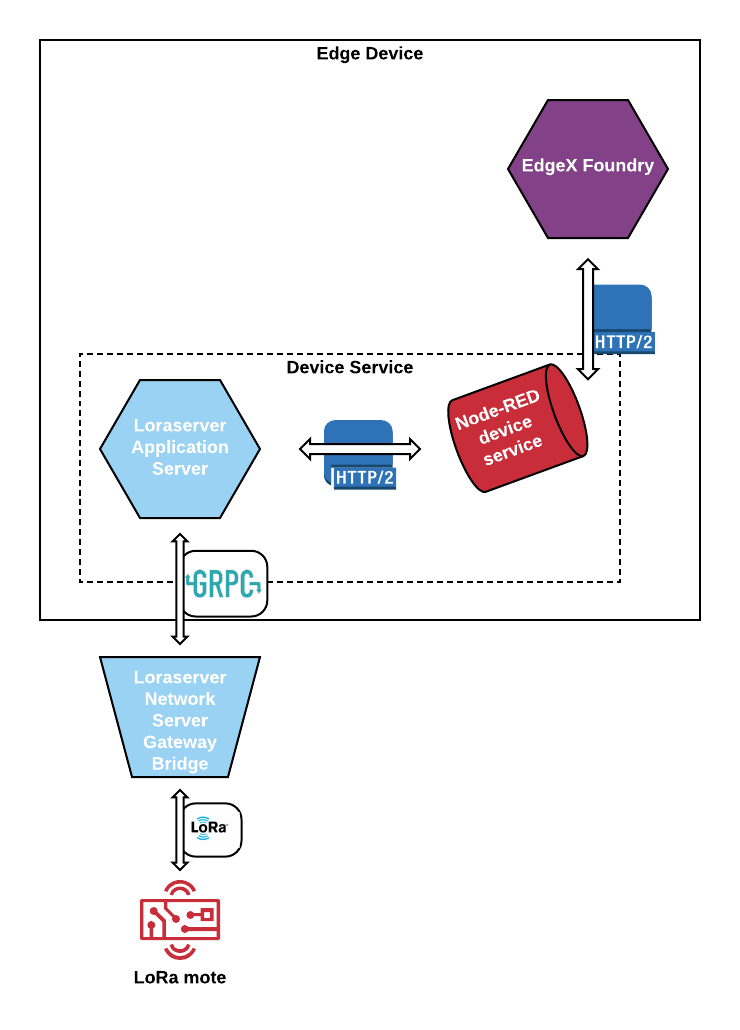
\includegraphics[width=0.7\textwidth]{images/dev_serv_arch.png}
    \caption{High level overview of the Device Service architecture showcasing the main components and their intercommunication protocols}
    \label{fig:device_service}
\end{figure}

The development of the edge service could follow two distincts routes. We could either use the go SDK of the EdgeX, which would serve as boilerplate for the EdgeX component, while we integrate the LoRa part or we could follow the specifications with a custom-tailored solution of our choice. We followed option 2 and instead of using the device service SDK\cite{device-service-sdk}, due to lack of experience with Golang, we opted to-partially-implement the EdgeX device service specification \cite{device-service-spec} in Node-RED.

This is due to the fact that what we needed was a middleware piece of software, that would expose 2 different APIs, one to the LoRa side and one to the EdgeX side. Node-RED is extremely streamlined for the creation of simple API based services, thus the device-service consists of a Node-RED microservice and a LoRaserver-app-server microservice. 

\subsection{Lora application Server}
loraserver.io offers already built images of the platforms, but it is unfortunate that the provided architectures do not include aarch64. Thus, we had to build the container with the application inside. Due to incompatible libraries with the architecture, it was impossible to build the application from source with Dockerfile, thus an intermediate solution was given. The Dockerfile would simply download the binary using \texttt{apt-get install} and then run it in a Alpine Linux BaseOS. Though our approach is not optimal, it is functional and adequate for the proof of concept. 


\subsubsection{Important Note}
A simplification that was made is the existence of the required Redis \& Postgresql server. In lieu of installing new instances in the Raspberry, it was opted that the app server will use the Redis and Postgresql servers that were already installed in Lorank8. It was necessary as Raspberry would not be able to support the load of all the services that we wanted to run.

This is important as the device-service, per the architectural demands, must be fully stateless and without dependencies. Thus, it would require that a total of 4 microservices (i.e node-red, LoRa app server, Postgresql, Redis) would be migrated so as the service provider to function as expected. In our scenario, there is a migration of 2 services (i.e node-red, app-server), while the other two are omitted. 

\subsection{Node-RED setup}
The best deployment method is to develop the node-RED locally and then extract the flow to the Node-RED runtime on the production machine. To install Node-RED locally, the user will use docker and follow the detailed documentation\cite{nodered-docker} provided by the development team. Using the Node-RED graphic editor, the user can start creating flows. Flows are different parts of the application that run in parallel and can be used to distribute the application logic and increase "code" readability.

The device-service state machine has only two states, the setup state and the normal operation state. We create a flow for each state for ease of use. When Node-RED service starts, the setup flow starts which registers the Node-RED service to both EdgeX and LoRa-app-server. This bootstrap phase is shown in Figures \ref{fig:devserv-boot1} and \ref{fig:devserv-boot2}. After the registration is complete, EdgeX and LoRa-app-server will start making requests to the API resources that we have defined in the second flow shown in Figure \ref{fig:devserv-norm}.

\subsection{Service setup state}
The flow starts with the inject node which outputs the first message as soon as Node-RED starts. Then, we make consecutive calls to the EdgeX platform in order to register the device service, as indicated in the EdgeX API walkthrough tutorial, with a small change: we don’t define a device addressable as indicated in the tutorial, but we define it in when provisioning a new device. To make the consecutive calls, all the HTTP POST requests bodies are defined at the start of the flow and saved as flow variables. Then, before each HTTP request node, we set the \textit{msg.url} and \textit{msg.payload} to the appropriate values. The url depends on the EdgeX service that the request is intended while the payload depends on the registration step. The reader is invited to research our github and see the structure of these payloads, we choose not to analyse further as they are use-case dependent. 

The same methodology is followed for the LoRa-App-Server registration as well, as shown in Figure \ref{fig:devserv-boot2}. The required steps to connect a sensor were found in the loraserver.io docs, but instead of the web interface, the RESTful API was used. Moreover, an HTTP integration is defined so that each time LoRa-app-server receives a reading, it is forwarded to a specific resource. This resource is in fact the Node-RED service that receives the data (south-side) and then makes an HTTP request to EdgeX (north-side). The network keys that were defined during the ABP setup of the Arduino mote are used in order for the application server to be able to decrypt the payloads that are received in the gateway.

\subsection{Service normal operation state}
During normal operation, the service has 5 active API HTTP resources, 4 are used by the EdgeX services and are defined in the EdgeX SDK specifications and one that is used by the LoRa-app-server to forward the LoRa mote readings. Currently the device service offers only one command to the EdgeX platform and the user, but it is possible to implement the whole SDK specification, offering any number of available commands.

\subsection{Containerization}
The containerization of the Node-RED service was based on the reference Dockerfile provided by the developers of the project\cite{nodered-docker}. What we have added is the placement of the \textit{flows.json}, \textit{package.json }and \textit{settings.json} inside the container so as 1) Node-RED loads our flows; 2) add a runtime argument to Node.js to limit the memory consumed by the process 3) configure Node-RED runtime for the implementation (e.g deactivate the GUI editor to reduce memory footprint). The placement of files inside the container is done at build time using the Dockerfile \texttt{}{COPY} command.

\bigskip \noindent
Finally, we comment on some fields of the configuration file of the Node-RED service:
\begin{itemize}
    \item \textbf{Flowfile:} filename of the json file with the flows
    \item \textbf{disableEditor:} if it set "\textit{True}", it disables editor to reduce memory footprint
    \item \textbf{contextStorage:} This is crucial as it dictates to Node-RED whether to save the defined variables (flow, global) in-memory or in-memory and in a file. We need the service to retain its status even after restart, thus we select the latter and configure it via contextStorage.
\end{itemize}

\newpage
\begin{sidewaysfigure}
    \centering
    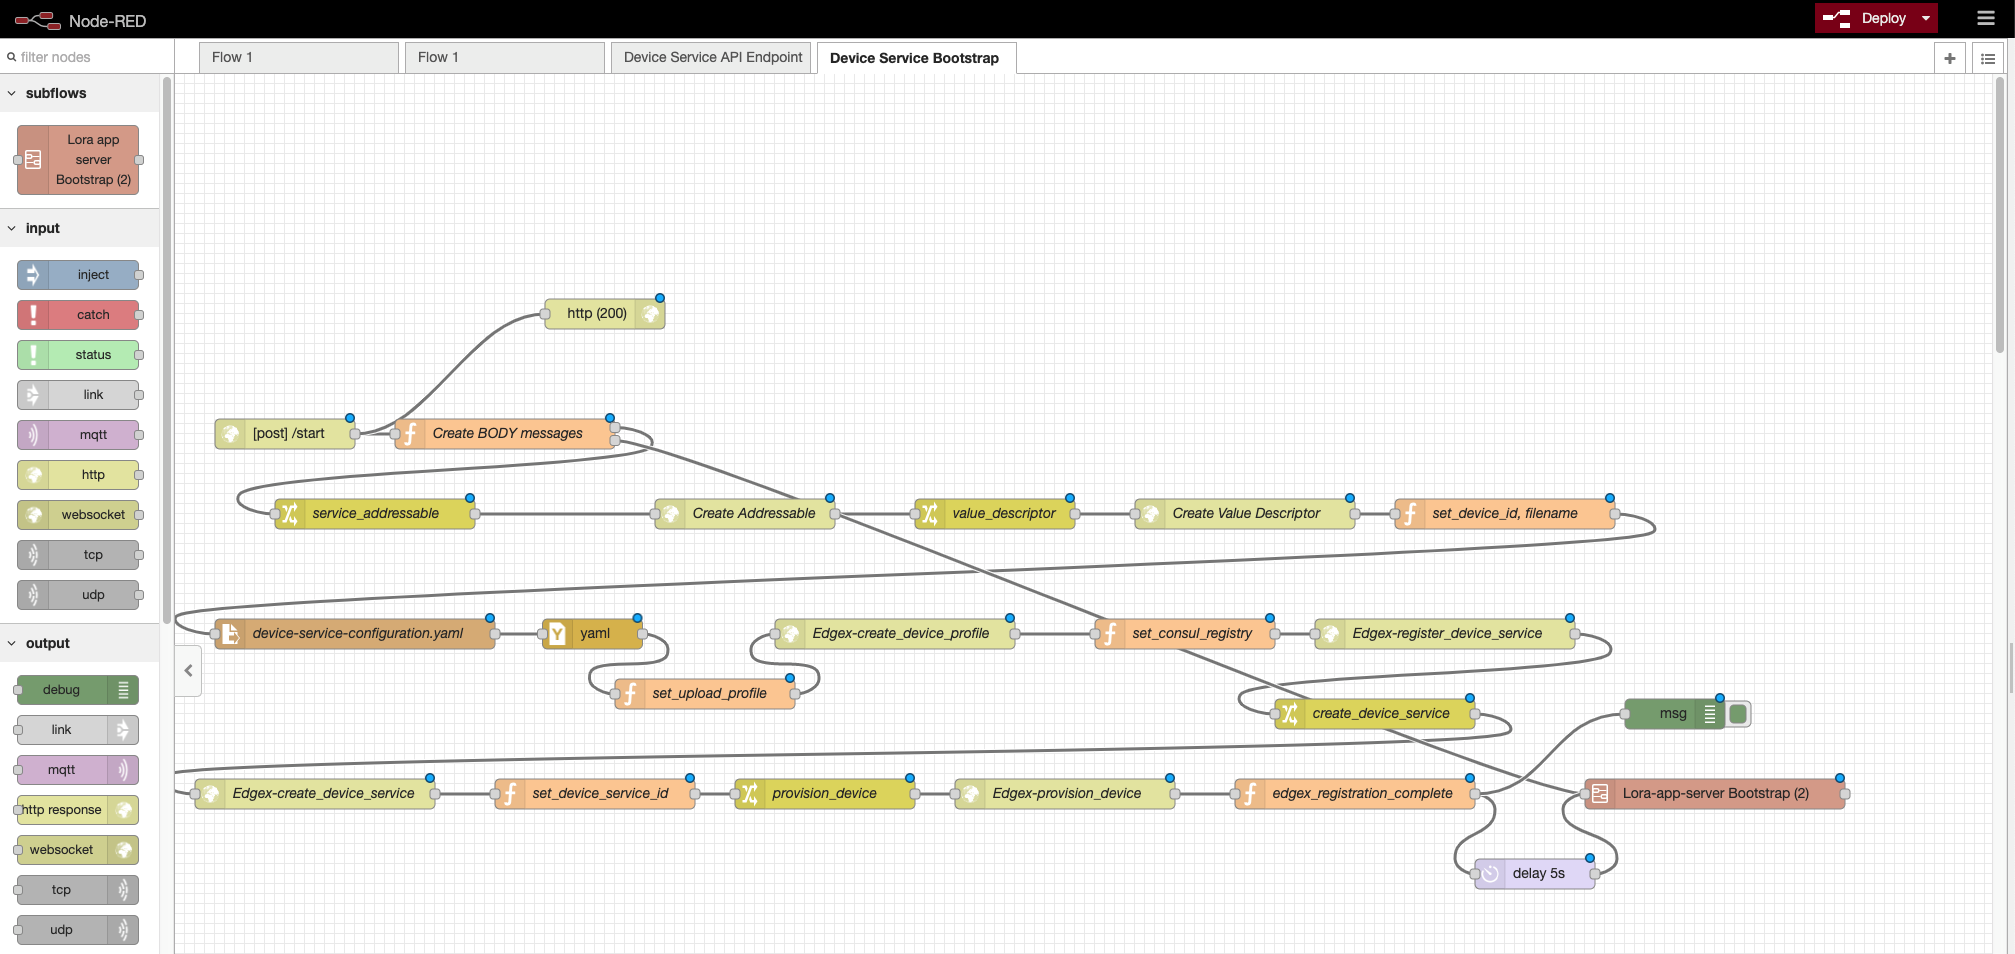
\includegraphics[width=\textwidth]{images/nodered_devserv_boot1.png}
    \caption{The bootstrap flow of the device service Node-RED instance for the EdgeX platform registration}
    \label{fig:devserv-boot1}
\end{sidewaysfigure}

\begin{sidewaysfigure}
    \centering
    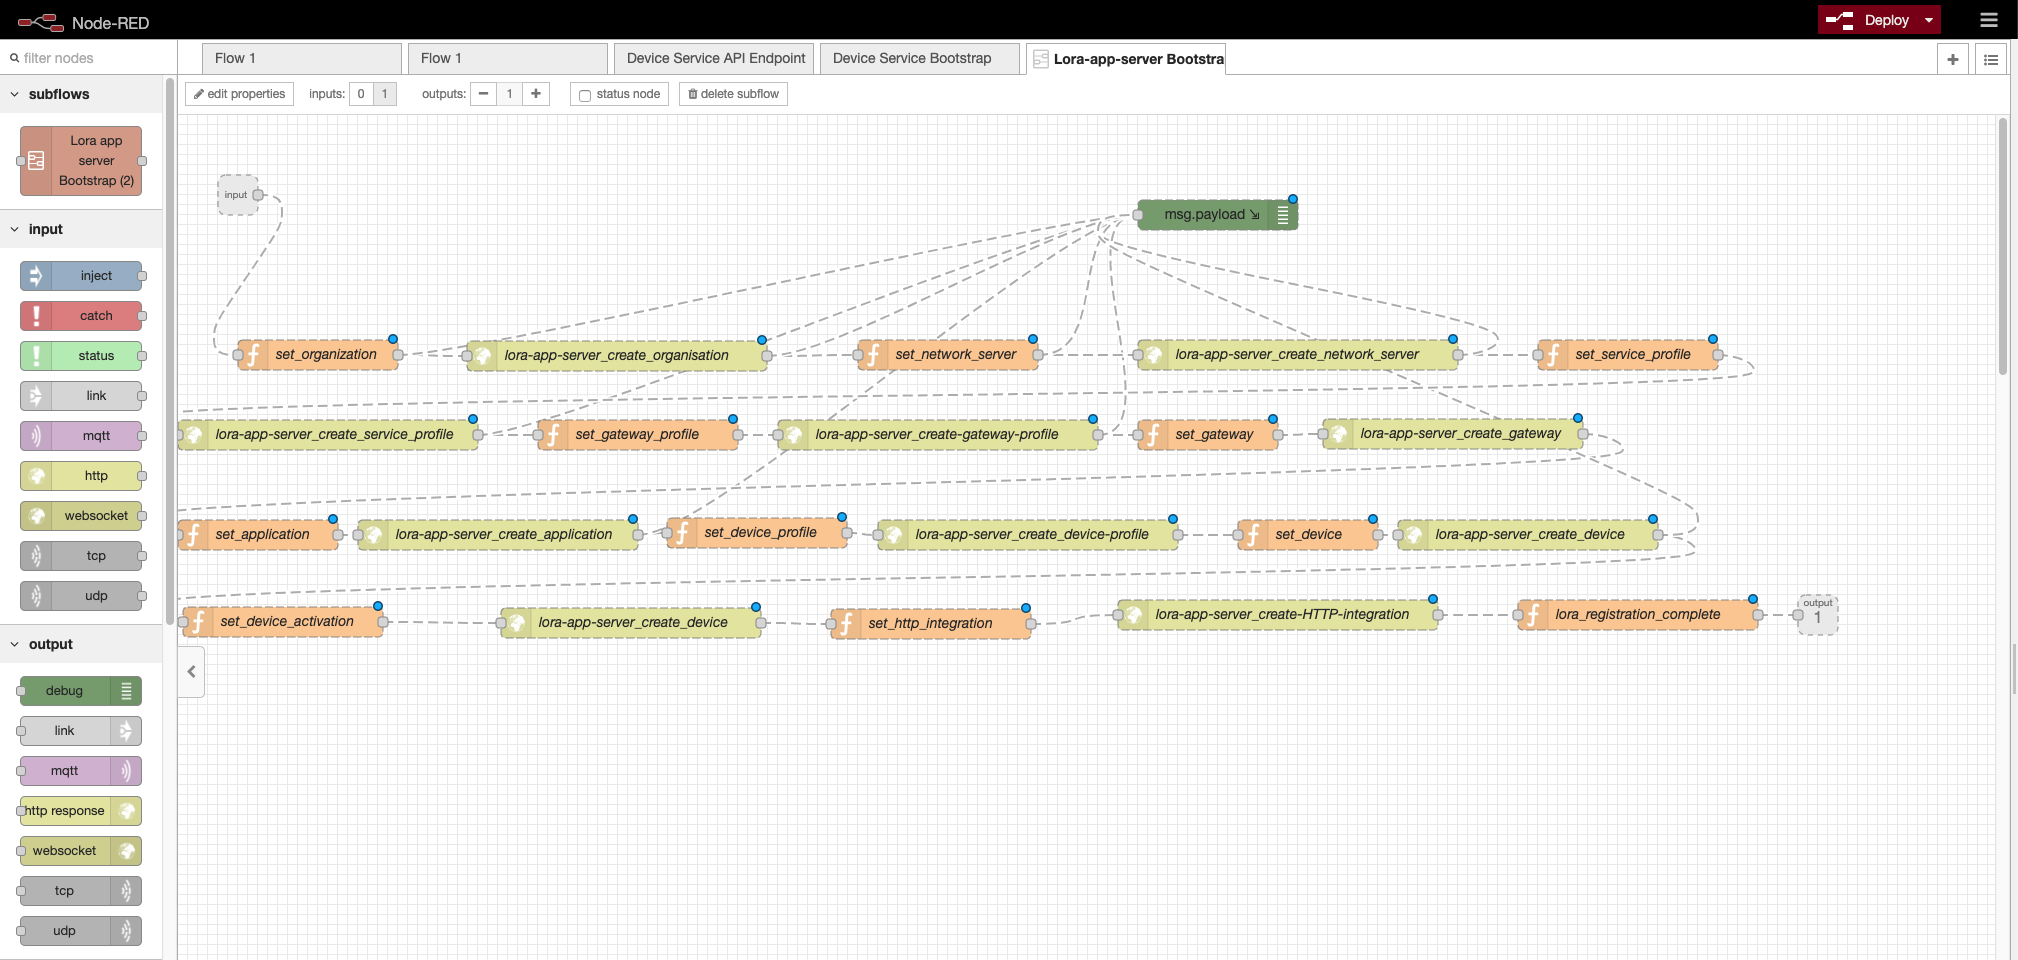
\includegraphics[width=\textwidth]{images/nodered_devserv_boot2.png}
    \caption{The bootstrap flow of the device service Node-RED instance for the LoRaserver application server registration}
    \label{fig:devserv-boot2}
\end{sidewaysfigure}

\begin{sidewaysfigure}
    \centering
    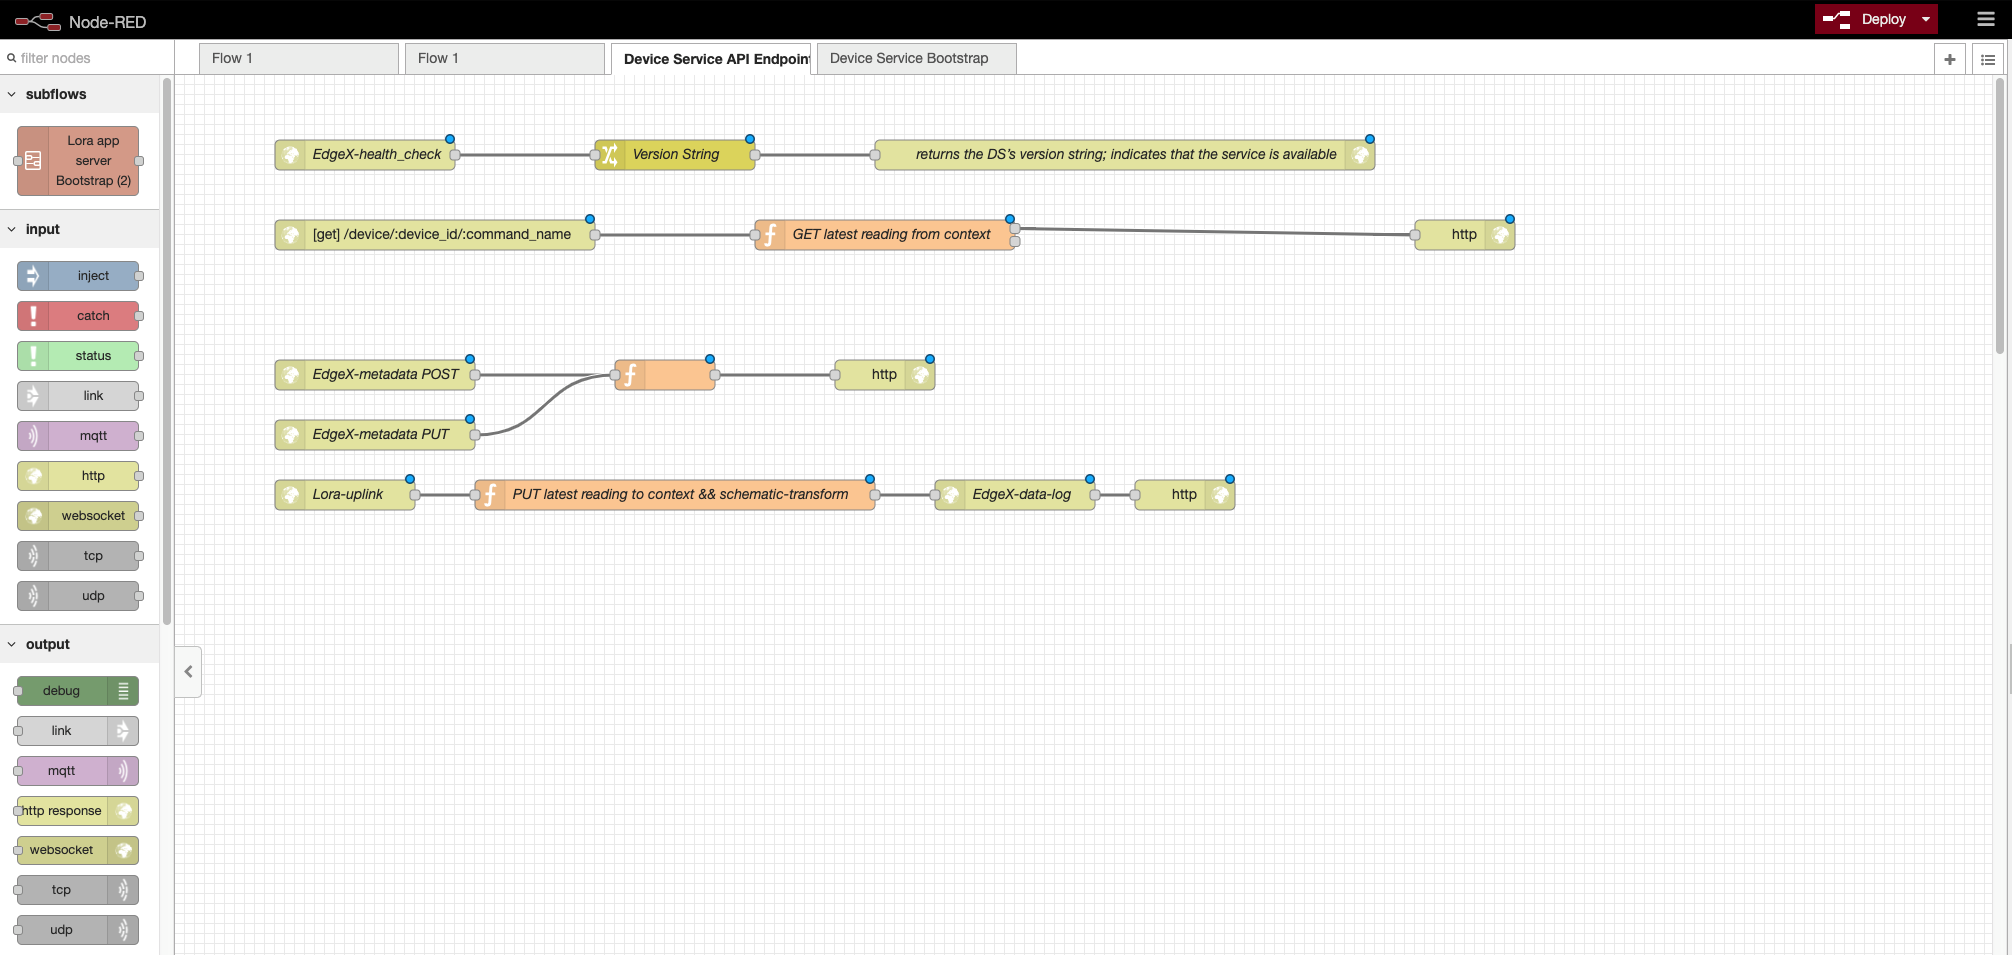
\includegraphics[width=\textwidth]{images/nodered_devserv_api.png}
    \caption{The normal operation flow of the device service is mainly a RESTful API}
    \label{fig:devserv-norm}
\end{sidewaysfigure}

\clearpage

\section{Orchestrator Component}

The orchestrator microservice\footnote{The implementation was partly based on the work of Athanasios Chamalidis, who developed a first implementation and contributed considerably regarding the implemented control of balena supervisor\cite{sakis}.} interfaces and implements multiple functionalities that belong to different services as defined in Architecture Chapter \ref{ch:system-architecture}, namely the \textit{migration service}, the \textit{orchestrator} and \textit{filecoin interface}. It is built in python and based on the flask framework. Flask enabled us to develop quickly while keeping the memory footprint considerably lower than node-red. The service can be logically divided into two parts, the orchestrator and the Filecoin/migration service. Each has its own RESTful API and they are loosely coupled, communicating through their APIs as being two different services. A , rather fancy, component overview can be seen in Figure \ref{fig:orchestrator_component} where we indicate the distinct services that interact in the orchestrator's migration service and the communication protocols.

\begin{figure}[h]
    \centering
    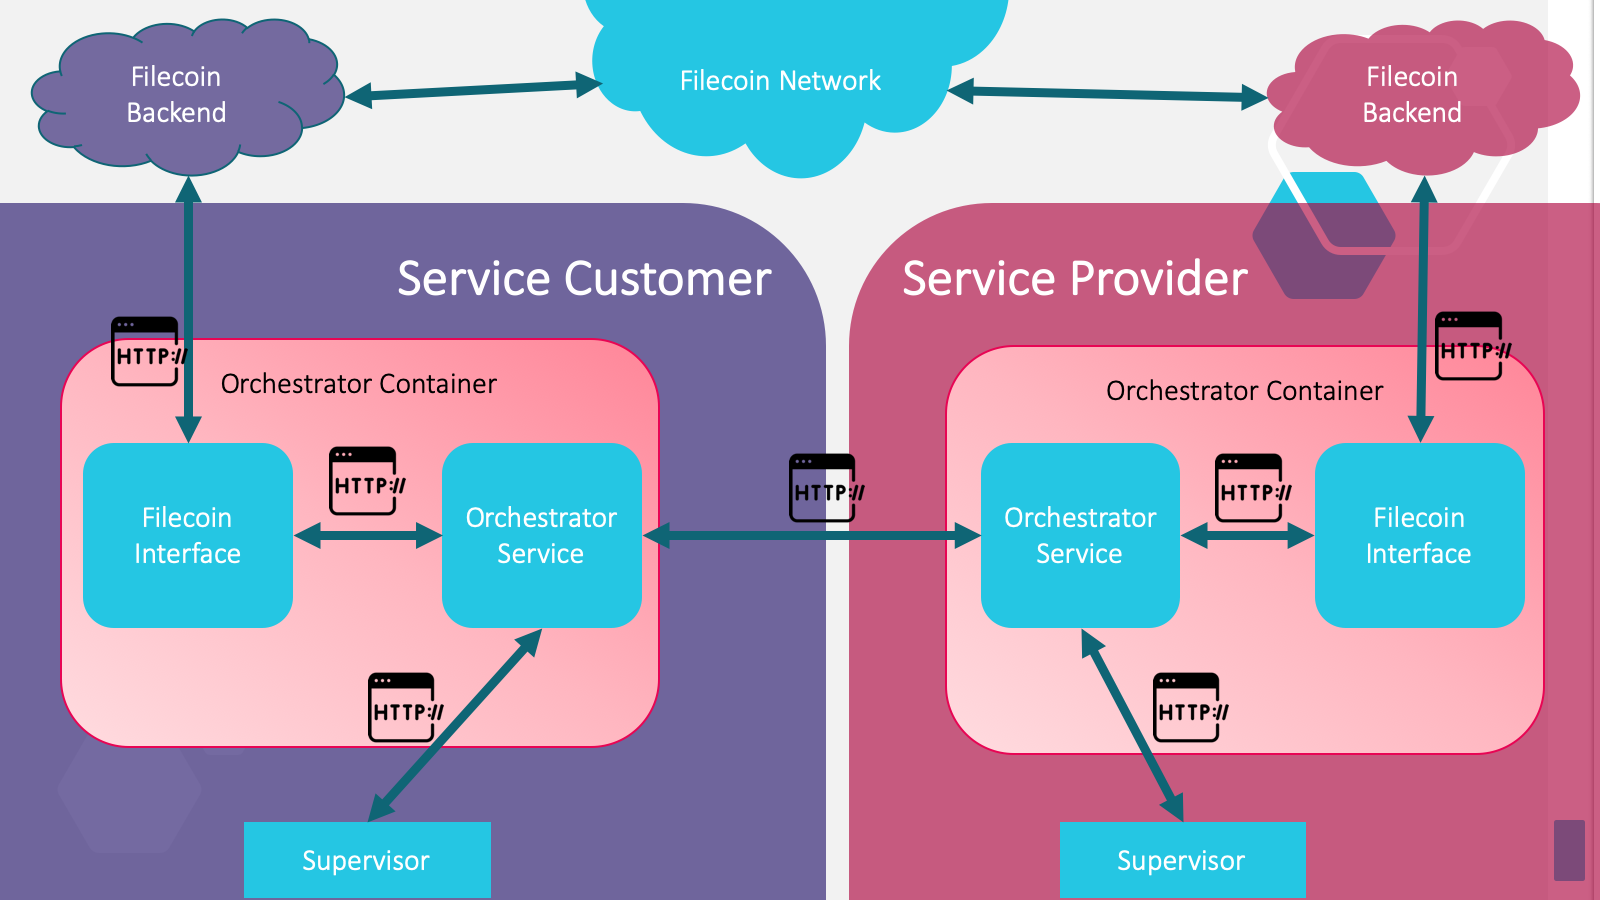
\includegraphics[width=1\textwidth]{images/orchestrator_comp.png}
    \caption{Component overview of the Orchestrator Microservice that is divided into 2 distinct services (orchestrator, filecoin interface)}
    \label{fig:orchestrator_component}
\end{figure}

\subsection{Orchestrator microservice}
\textbf{Functionality:}
\begin{itemize}
    \item Request Filecoin interface to save a container image to the Filecoin DSN
    \item Request Filecoin interface to download a container image from the Filecoin DSN
    \item Load image to balenaEngine
    \item Get balena supervisor state
    \item Set balena supervisor state 
    \item Save \& Load orchestrator from and to a file
    \item Communicate with another orchestrator service and create a service contract
    \item Provide resources for orchestrators inter-communication and Filecoin interface update
\end{itemize}

\subsection{Orchestrator API Resources}

\begin{table}[H]
\centering
\begin{tabular}{|l|l|lll}
\cline{1-2}
\multicolumn{2}{|l|}{{\ul }}                                                                                   &  &  &  \\
\multicolumn{2}{|l|}{\textit{/orchestrator/service\_customer/image/status}}                                    &  &  &  \\ \cline{1-2}
\textbf{{[}GET{]}}  & get the status of all the images of the Edge that are/will be used in a service contract &  &  &  \\ \cline{1-2}
\textbf{{[}POST{]}} & examples:                                                                                &  &  &  \\
                    & \{                                                                                       &  &  &  \\
                    & imageId: 16935cab-2de3-4014-b0f7-3f15eca09bdc16935cab-2de3-4014-b0f7-3,                  &  &  &  \\
                    & imageHash: 7kg8sdf03jdfh9hfsf49h0sdf,                                               &  &  &  \\
                    & status: STORED \# status from [STORED, COMMITED]                                     &  &  &  \\
                    & \}                                                                                       &  &  &  \\ \cline{1-2}
\end{tabular}
\caption{Orchestrator service, REST resource: /orchestrator/service\_customer/image/status}
\end{table} %/orchestrator/service\_customer/image/status
\begin{table}[H] % orchestrator/service\_provider/image/status
\centering
\begin{tabular}{|l|l|lll}
\cline{1-2}
\multicolumn{2}{|l|}{{\ul }}                                                                  &  &  &  \\
\multicolumn{2}{|l|}{\textit{/orchestrator/service\_provider/image/status}}                   &  &  &  \\ \cline{1-2}
\textbf{{[}GET{]}}  & get the status of all images that belong to 3rd parties                 &  &  &  \\ \cline{1-2}
\textbf{{[}POST{]}} & examples:                                                               &  &  &  \\
                    & \{                                                                      &  &  &  \\
                    & imageId: 16935cab-2de3-4014-b0f7-3f15eca09bdc16935cab-2de3-4014-b0f7-3, &  &  &  \\
                    & status: DOWNLOADED                                                      &  &  &  \\
                    & \}                                                                      &  &  &  \\ \cline{1-2}
\end{tabular}
\caption{Orchestrator service, REST resource:  orchestrator/service\_provider/image/status}
\end{table}
\begin{table}[H] %/orchestrator/service\_provider/contract
\begin{tabular}{|l|l|lll}
\cline{1-2}
\multicolumn{2}{|l|}{{\ul }}                                                               &  &  &  \\
\multicolumn{2}{|l|}{\textit{/orchestrator/service\_provider/contract}}                    &  &  &  \\ \cline{1-2}
\textbf{{[}GET{]}}  & get all contracts from the Edge in which it acts as service provider &  &  &  \\ \cline{1-2}
\textbf{{[}POST{]}} & examples:                                                            &  &  &  \\
                    & \{                                                                   &  &  &  \\
                    & edgeId: asdfasdfa,                                                   &  &  &  \\
                    & imageName:asdfadsfas,                                                &  &  &  \\
                    & imageHash:adsfasfda,                                                 &  &  &  \\
                    & config: configFile.json                                               &  &  &  \\
                    & \}                                                                   &  &  &  \\ \cline{1-2}
\end{tabular}
\caption{Orchestrator service, REST resource:  /orchestrator/service\_provider/contract}
\end{table}
\begin{table}[H]
\centering
\begin{tabular}{|l|l|lll}
\cline{1-2}
\multicolumn{2}{|l|}{{\ul }}                                                                                         &  &  &  \\
\multicolumn{2}{|l|}{\textit{/orchestrator/service\_customer/contract/testing}}                                      &  &  &  \\ \cline{1-2}
\textbf{{[}GET{]}}  & get all contracts from the Edge in which it acts as service customer                           &  &  &  \\ \cline{1-2}
\textbf{{[}POST{]}} & examples:                                                                                      &  &  &  \\
                    & \{                                                                                             &  &  &  \\
                    & imageName: LoRa-device-service,                                                                &  &  &  \\
                    & fileName: LoRa-device-service.tar                                                              &  &  &  \\
                    & duration: 7 \#days                                                                             &  &  &  \\
                    & \}                                                                                             &  &  &  \\
                    & \# Resource that is used to start the migration \& contract process, for testing purposes only &  &  &  \\ \cline{1-2}
\end{tabular}
\caption{Orchestrator service, REST resource:  /orchestrator/service\_customer/contract/testing}
\end{table}%/orchestrator/service\_customer/contract/testi
\begin{table}[H] %orchestrator_health
\begin{tabular}{|l|l|lll}
\cline{1-2}
\multicolumn{2}{|l|}{{\ul }}                                         &  &  &  \\
\multicolumn{2}{|l|}{\textit{orchestrator/health}}                   &  &  &  \\ \cline{1-2}
\textbf{{[}GET{]}} & get service status message                      &  &  &  \\
                   & Response:                                       &  &  &  \\
                   & \textit{Status Message: “orchestrator v.0.1.2”} &  &  &  \\ \cline{1-2}
\end{tabular}
\caption{Orchestrator service, REST resource:  /orchestrator/health}
\end{table}

\subsection{Orchestrator's Migration Process}

The orchestrator is built around the Orchestrator class and enables the Edge to function both as a service provider and as a service customer. We give a succinct description of some parts of the code:
\begin{itemize}
    \item \texttt{self.contract\_services\_customer, self.contract\_services\_provider:} data structures (dictionaries) that contain the contracts depending on the role of the orchestrator Edge device.
    \item \texttt{set\_state():} 1) generate device state, by concatenating current state and the new service 2) save orchestrator state in file\footnote{It is necessary because when setting a new state, all unchanged containers restart. We use the volumes file persistency to persist the state of the orchestrator.} 3) set new state.
    \item \texttt{contract\_setup():} updates the contact\_services\_provider dictionary and requests the services image from Filecoin interface
    \item \texttt{check\_contract():} verifies whether the contract activation parameters exist and executes the contract if they are fulfilled. In the current implementation, it is hardcoded to verify the online status of the service customer’s Edge device.
\end{itemize}

The service migration process is initiated manually by the developer by requesting a REST resource and the public URL on where the endpoint of the above resources rest is hardcoded into each Orchestrator service. The process is described in detail by Figures \ref{fig:service_mig_1}, \ref{fig:service_mig_2} where the migration is modeled in a UML sequence diagram. Note that Figure \ref{fig:service_mig_2} is a continuation of Figure \ref{fig:service_mig_1} and in fact the service customer orchestrator entity starts activity in diagram \ref{fig:service_mig_1} and finishes in diagram \ref{fig:service_mig_2}. The implemented process is algorithmically described in Section \ref{st:balena-filecoin}.

\clearpage
\begin{sidewaysfigure}
    \centering
    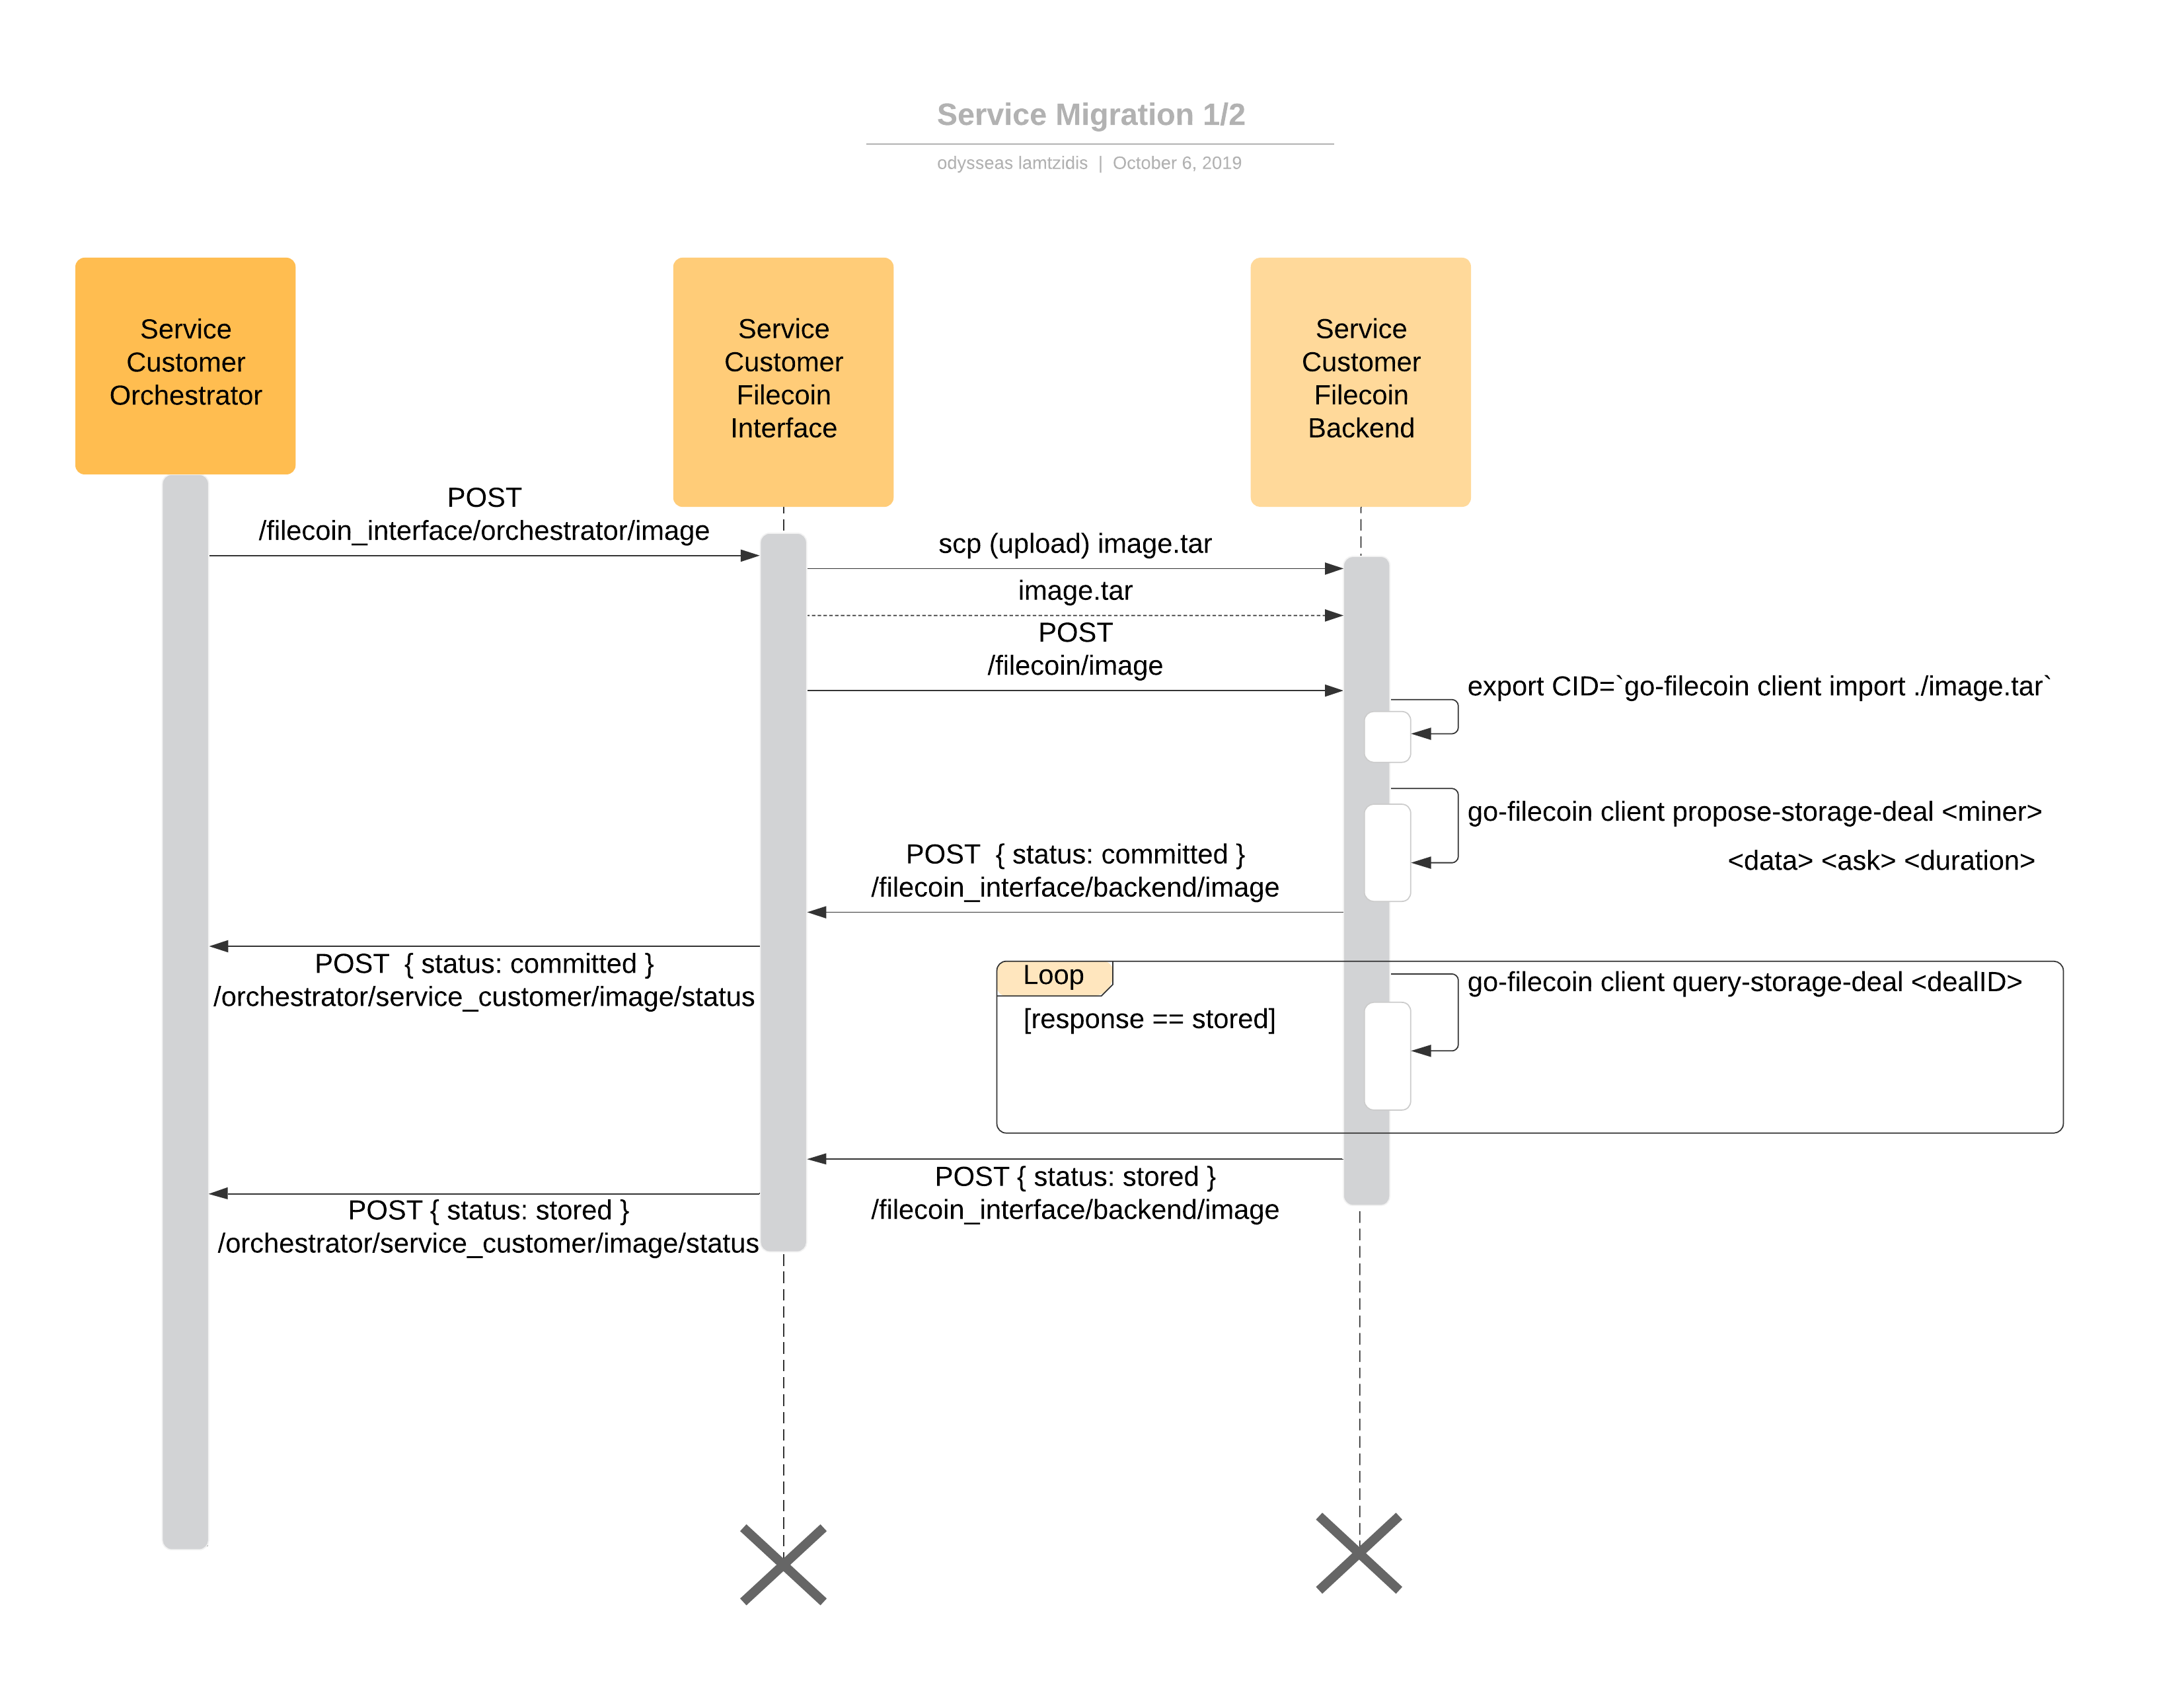
\includegraphics[width=0.9\textwidth]{images/service_mig_1.png}
    \caption{The sequence UML of the migration process, initiated by the Service Customer}
    \label{fig:service_mig_1}
\end{sidewaysfigure}

\begin{sidewaysfigure}
    \centering
    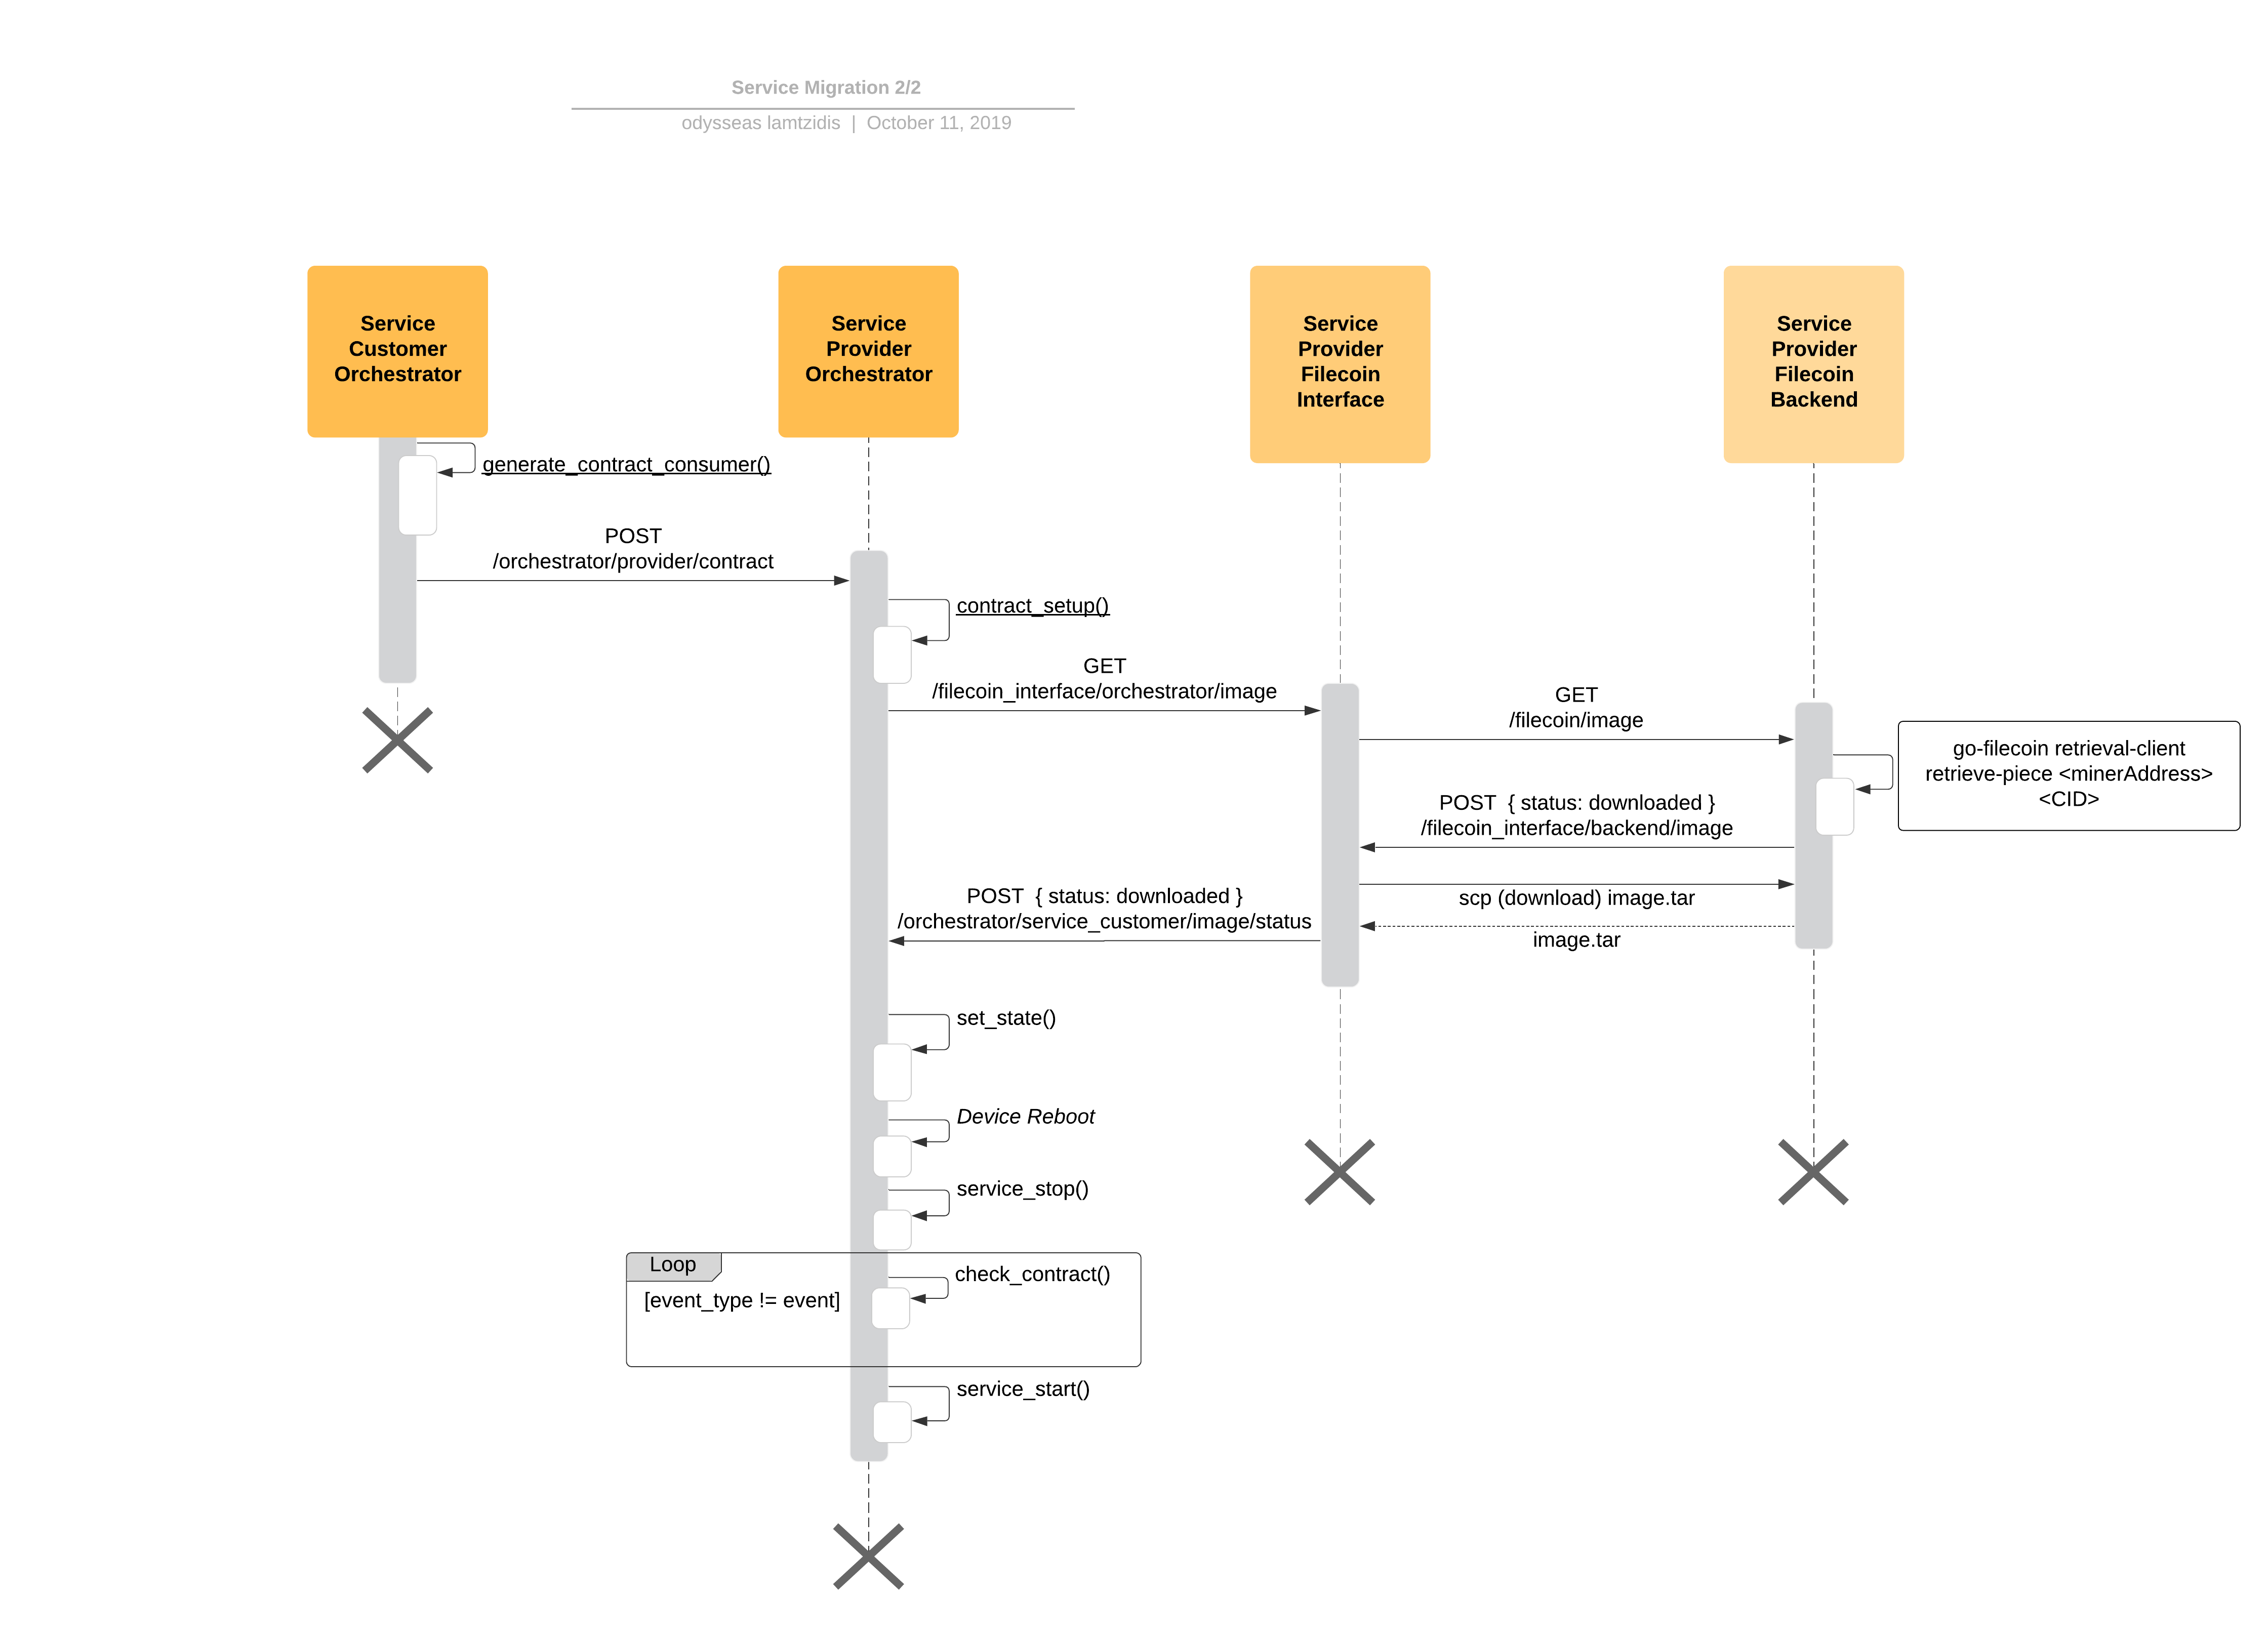
\includegraphics[width=0.9\textwidth]{images/service_mig_2.png}
    \caption{The sequence UML of the migration process (contd.) follow up by service provider}
    \label{fig:service_mig_2}
\end{sidewaysfigure}

\clearpage
\subsection{Filecoin Interface component}

It has a dual role, fulfilling the roles of migration service and the Filecoin network interface. 

As mentioned in Section \ref{st:filecoin}, Filecoin is currently in alpha version and therefore demands high computational resources, rendering it impossible to be run on Raspberry Pi 3. Moreover, the current Official API implementation is incomplete and could possibly have a considerate amount of bugs, decreasing considerably our speed of development. 

Thus, we developed our own Filecoin API, by developing a node-RED application that runs on a cloud Linux server and exposes the Filecoin functionality that we require using 2 RESTful HTTP resources. We call it filecoin interface backend service. The backend service extracts information from the HTTP requests and translates them into Filecoin-CLI commands, functioning exclusively as a wrapper around Filecoin. A screenshot of Node-RED web editor and the aforementioned flow can be seen in Figure \ref{fig:filecoin_backend}.

\noindent
The REST interface of the filecoin interface component is surmised bellow:
% Please add the following required packages to your document preamble:
% \usepackage[normalem]{ulem}
% \useunder{\uline}{\ul}{}
\begin{table}[H]
\centering
\begin{tabular}{|l|l|lll}
\cline{1-2}
\multicolumn{2}{|l|}{{\ul }} &  &  &  \\
\multicolumn{2}{|l|}{\textit{/filecoin\_interface/backend/image}} &  &  &  \\ \cline{1-2}
\textbf{{[}POST{]}} & examples: &  &  &  \\
 & \textit{\{} &  &  &  \\
 & imageid: 16935cab-2de3-4014-b0f7-3f15eca09bdc16935cab-2de3-4014-b0f7-3, &  &  &  \\
 & imageHash: 7kg8sdf03jdfh9hfsf49h0sdf, &  &  &  \\
 & status: STORED  \# status from {[}STORED, COMMITTED, READY2DOWNLOAD{]} &  &  &  \\
 & \} &  &  &  \\ \cline{1-2}
\end{tabular}
\caption{Filecoin Interface service, REST resource: /filecoin\_interface/backend/image }
\end{table} 

\begin{table}[H] %filecoin/orchestrator/image
% \centering
\begin{tabular}{|ll|lll}
\cline{1-2}
\multicolumn{2}{|l|}{{\ul }} &  &  &  \\
\multicolumn{2}{|l|}{\textit{/filecoin\_interface/orchestrator/image}} &  &  &  \\ \cline{1-2}
\multicolumn{1}{|l|}{\textbf{{[}GET{]}}} & \{ &  &  &  \\
\multicolumn{1}{|l|}{} & imageName: LoRa-device-service, &  &  &  \\
\multicolumn{1}{|l|}{} & imageHash: 7kg8sdf03jdfh9hfsf49h0sdf, &  &  &  \\
\multicolumn{1}{|l|}{} & minerAddress: QmfVk1c4Byn5E5He6Sk7Y8NTRNUtfBE7yhJedpDwi94rat &  &  &  \\
\multicolumn{1}{|l|}{}  & \} &  &  &  \\ \cline{1-2}
\multicolumn{1}{|l|}{\textbf{{[}POST{]}}} & \{ &  &  &  \\
\multicolumn{1}{|l|}{} & imageName: LoRa-device-service, &  &  &  \\
\multicolumn{1}{|l|}{} & storageDuration: 7 \#days, &  &  &  \\
\multicolumn{1}{|l|}{} & fileName: LoRa-device-service.tar, &  &  &  \\
\multicolumn{1}{|l|}{} & \} &  &  &  \\ \cline{1-2}
\end{tabular}
\caption{Filecoin Interface service, REST resource: /filecoin\_interface/orchestrator/image}
\end{table}
% Please add the following required packages to your document preamble:
% \usepackage[normalem]{ulem}
% \useunder{\uline}{\ul}{}
\begin{table}[H]
% \centering
\begin{tabular}{|l|l|lll}
\cline{1-2}
\multicolumn{2}{|l|}{{\ul }} &  &  &  \\
\multicolumn{2}{|l|}{\textit{/filecoin\_interface/backend/error}} &  &  &  \\ \cline{1-2}
\textbf{{[}POST{]}} & \textit{\{} &  &  &  \\
 & errorObject: error.json, &  &  &  \\
 & code: 404, &  &  &  \\
 & message: can't find miner with minerId "Qj3249fj... &  &  &  \\
 & \} &  &  &  \\ \cline{1-2}
\end{tabular} %/filecoin\_interface/backend/error
\caption{Filecoin Interface service, REST resource: /filecoin\_interface/backend/error}
\end{table}

\begin{table}[H]
\begin{tabular}{|l|l|lll}
\cline{1-2}
\multicolumn{2}{|l|}{{\ul }}                                            &  &  &  \\
\multicolumn{2}{|l|}{\textit{filecoin\_interface/health}}               &  &  &  \\ \cline{1-2}
\textbf{{[}GET{]}} & get service status message                         &  &  &  \\
                   & Response:                                          &  &  &  \\
                   & \textit{Status Message: “filecoin interface v.01”} &  &  &  \\ \cline{1-2}
\end{tabular}%
\caption{Filecoin Interface service, REST resource: /filecoin\_interface/health}
\end{table} % filecoin_health

\begin{sidewaysfigure}
    \centering
    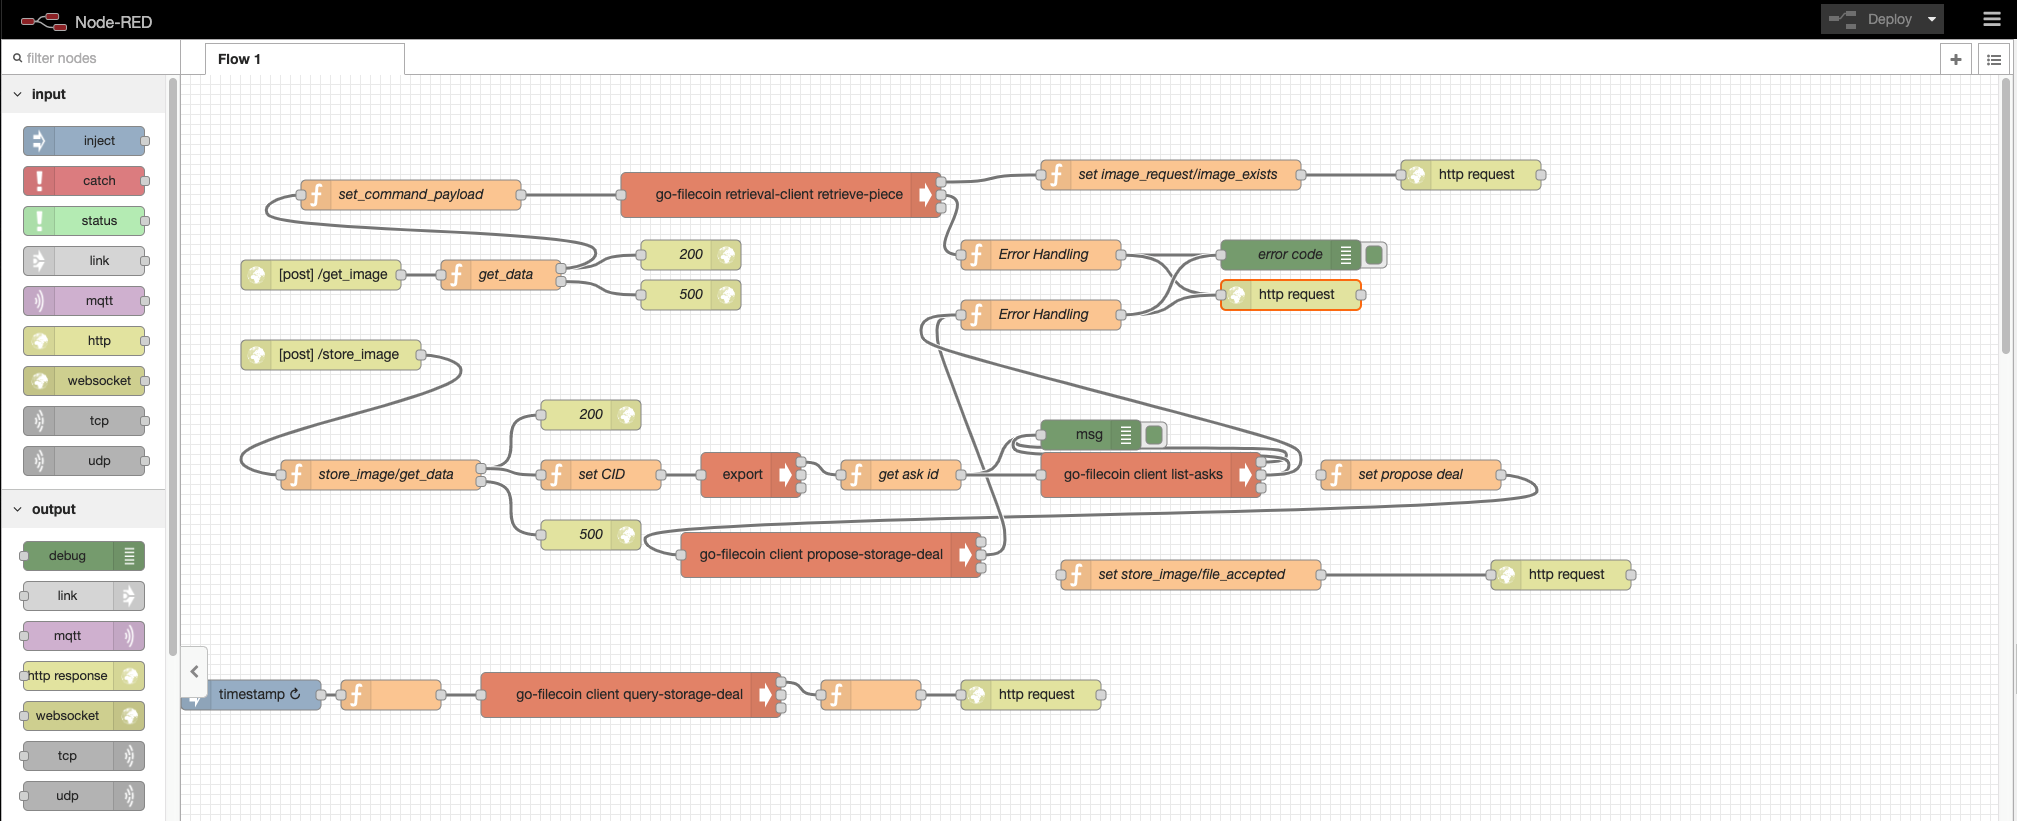
\includegraphics[width=0.9\textwidth]{images/nodered_backend.png}
    \caption{The Filecoin Backend service is a Node-RED instance with a single flow, a RESTful API}
    \label{fig:filecoin_backend}
\end{sidewaysfigure}

Finally we note that we don’t use HTTP to send the images from the edge device to the backend and vice-versa. This is because when uploading using the POST HTTP method (e.g via curl), the whole file is buffered into the memory before being uploaded. This is hugely inefficient, since our Raspberry is extremely memory constrained, taking into consideration the number of services which run concurrently.

Thus, we opted to use \texttt{scp} (secure copy) which can copy files from and to a remote server using the ssh protocol. The file is sent in buffered chunks, thus the memory footprint is kept considerably lower. While this implies trust between the two computers (as we use the same credentials used for ssh), there are methods to make it work (e.g create a user with zero privileges) or we could switch to ftp which is less efficient but still expected to be feasible in our setup.

At a high level, Filecoin Interface sends an image using scp and informs Filecoin backend of the existence of the image. Conversely, when requesting an image, Filecoin interface will request the image from the backend service, the backend service will proceed to download it from the Filecoin DSN and finally it will notify Filecoin Interface so as it uses scp to download it.



 \clearemptydoublepage
 
 \chapter{Discussion} \label{ch:discussion}
\markboth{Discussion}{}

There are several assumptions and simplifications that are made in this thesis, especially in implementation Chapter \ref{ch:implementation}. Although we believe that they are outside of the scope of this thesis, we believe it’s important to reiterate them so as the reader is lead to a solid conclusion and better grasp of our vision for any future steps.

The first and foremost need is to verify the problematic and find the appropriate business use-case. Business, in the sense that our proposed architecture can solve a real world problem and provide value to the user. Preliminary research has indicated that, indeed, there is such a need, taking into account the growing number of IoT devices and the need for efficient and low-latency processing and decision-making in a scalable manner, we still believe that discussion with key industry leaders can lead to more specific results and use cases.

Moreover, the defined architecture is still under research whether it is the appropriate means for our end goal. It is true that the container technology has found a unique balance between complete isolation and computational overhead, enabling us to implement it even in the most weak computational systems, like the  Raspberry pi micro-computer. But, it remains to be seem whether it will be usable between hostOs and containers that may belong to different stakeholders, possibly without trust.

The final system was designed as a proof of concept and implemented/tested inside a lab environment. However, towards a more business-oriented implementation, a complete assessment is required not only for the security of the overall system but also for its individual components. We understand that there are important security implications regarding the use of containers in a multi-tenancy scenario with possible hostile HostOs and/or hostile containers, but we envisage to perform such an analysis before continuing with further development.

Finally, the services mentioned in the implementation Chapter \ref{ch:implementation} were developed as a proof of concept and thus they do not conform to production-ready standards, such as PEP syntax style or programming paradigms such as parallel programming. The reader is advised to re-implement the services for replication purposes, using our implementation as a reference point for functionality.


\section{Assumptions}

Assumptions were also made in the implementation to be able to narrow the broad spectrum of this thesis.

The loraserver.io infrastructure was divided into a part that is assumed to exist in any LoRa capable Edge device and a part that realises the application logic, this has certain implications:

\begin{enumerate}
    \item Security wise our assumption was correct as the application server is the sole capable of decrypting the LoRa payload (due to the application network key). 
    \item In the implemented architecture, the application server should have it’s own dedicated and isolated databases but we opted to use the lorank loraserver’s for efficiency. This is security-wise wrong, as the owner of the databases is the IoT Edge of the service provider and thus he would have access to possibly sensitive information.
    \item Filecoin is still in early alpha, offering no stable release as of the moment of writing (21/9). This means that the implementation, could break with any new release and while it is acceptable for a proof of concept, we can’t expect to build a prototype with Filecoin as a critical component.
    \item The use of Filecoin is to enhance the autonomy of the IoT Edge, as the Edge has direct access to the Storage Layer. Although using the backend Filecoin Interface, we render our argument moot, for the same reasons as in 3), we feel that it is an acceptable assumption.
    \item The developed scripts do not adhere to programming best practices (such as syntax specifications) and where made with development speed at mind. They will be done re-programming from the ground up for a prototype to emerge.
\end{enumerate}

We believe that it is correct to assume that only the application layer of the LoRa infrastructure will need to be sent from the service customer to the service provider. This is because, in order for the service provider to be able to support the management of LoRa devices, it is not only necessary to have all the required hardware as also have an implementation of the packet forwarder. Moreover, it is assumed that the service providers and customers will use the same LoRawan infrastructure, namely the suite offered by loraserver.io. Thus, we believe it’s logical to assume that the contract between the Edges will dictate the interfacing of the service customer's services on the pre-existing infrastructure.

By underlining these simplifications and assumptions ,we believe that the reader will be able to better visualise our implementation goals and whether there is a need for further research and development regarding our project and approach. Future steps that we feel are important to showcase, are presented in Chapter \ref{ch:future-work}.

 \clearemptydoublepage
 
 \chapter{Results} \label{ch:results}
\markboth{Results}{}

The implementation showcases a successful handover of sensors by means of transferring the device-service container from one failed Edge to the next one in range. We have successfully created a stateless service that will perform the exact same functionality without requiring to sustain a specific state, as long as the environment provides the necessary infrastructure for the service to interface.

Moreover, we have combined an array of different and innovative technologies to construct the architecture on a new field with little relevant research. We feel that the combination of docker technology in the form of balenaOS and Filecoin as a decentralized storage for image containers can create a new interesting approach towards a network of IoT Edge computers.   

With the current implementation, two Edge devices that have the exact same structure as described in Implementation Chapter \ref{ch:implementation}, when manually activated, will enter into a digital contract and transfer services over Filecoin from the service customer to the service provider. The service provider monitors the service customer’s activity and in case it detects that it is offline, it starts the containers as indicated in the contract and the configuration file.

Thus, the implementation successfully showcases the rent of resources from one Edge (service provider) device to another (service customer) by means of running containers sent by the service customers on the service provider’s device which will retain it’s normal functionality for all the duration of this process.

Finally, during the development of the implementation, we actively participated in the online communities of the open source projects that we used, making contributions in the process. These contributions belong mainly to the field of documentation and functionality improvements, we also showcased how different platforms can be integrated together, namely Balena and EdgeX\cite{edgexbalenaodys}. Our work with EdgeX resulted in an invitation to Architect's day of the EdgeX conference, where the future of the project and architectural matters are discussed. We are extremely glad for contributing to these projects and we hope that this thesis will serve as stepping stone for others, both from the development and academic communities.
 \clearemptydoublepage
 
 \chapter{Future Work} \label{ch:future-work}
\markboth{Future Work}{}

Regarding the future, we believe that this thesis is only the starting point of an innovative approach towards a new paradigm for the democratization of IoT Edge Computing and the Internet of Things. Having introduced a high level architecture, our first objective is to continue the research and create the proper specifications for the entire architecture, including the components ,the described processes and proceed to the verification and validation of the proposed system. On top of that, there are various elements that are presented or mentioned in our work that merit more thorough research, namely in the areas of security, distributed systems and Internet of things.

We find that the following areas are ripe for research:
\begin{itemize}
    \item Required Resources estimation for a given container image
    \item Resources evaluation for a given Edge device
    \item A Filecoin light client ( “light” = It doesn’t need to download the entirety of the blockchain)
    \item A “Chinese” wall between containers and hostOS, keeping the good parts of the container technology while eliminating security issues between a hostile host and a trusted container or 
    vice-versa.
    \item Container intercommunication over a hostile environment
    Edge \& Central Arbitrator architecture

\end{itemize}

We envisage a system where various stakeholders can use established Edge Nodes devices to manage their IoT sensors and constrained devices, decoupling in essence the infrastructure owner and the end-user. Moreover, this model can be used in the cloud layer, where stakeholders will rent fully functional IoT platform systems (as opposed to services such as AWS where you rent cloud resources) to manage their IoT fleet.

\begin{figure}[h]
    \centering
    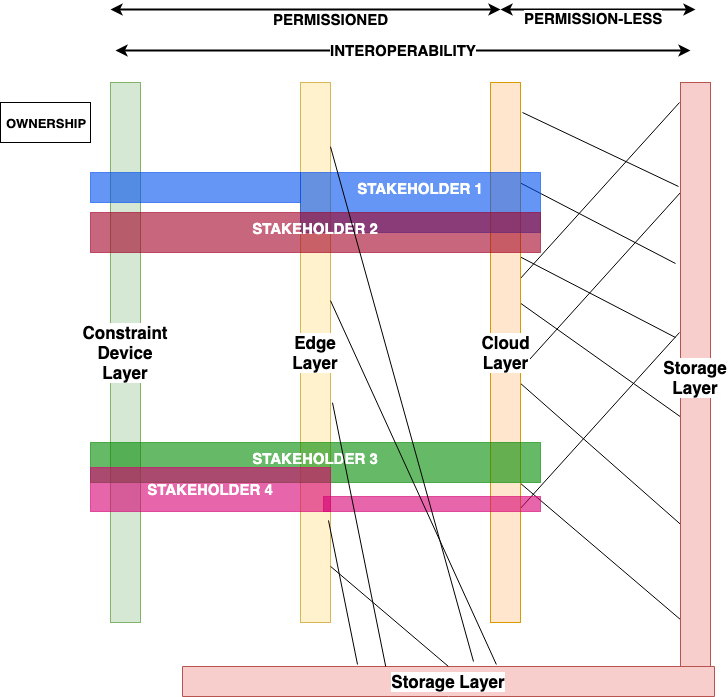
\includegraphics[width=0.9\textwidth]{images/layers_now_v2.png}
    \caption{The IoT reference architecture as a series of layers, partly decentralized }
    \label{fig:layers_now}
\end{figure}

In Figure \ref{fig:layers_now} we demonstrate the 4 distinct layers of the system, showcasing the subsystems that act in a permissioned \& trusted environment and the Storage Layer which does not. We also demonstrate the vertical slices of different stakeholders, where the overlap indicates that they are in fact participating in a contract. The different lines between the Cloud Layer and the Storage Layer illustrate that any stakeholder from the Cloud Layer can connect and store, in fact, to any stakeholder in the Storage Layer.
 
While the current implementation and architecture features a centralized system, we foresee that the breakthrough will be achieved in a fully decentralized system, where Edge \& Cloud nodes will be rented dynamically and the hand-over will be done almost seamlessly. Exploiting Distributed Ledger Technologies (such as the blockchain) we envisage a system where any stakeholder can participate and offer or demand Edge \& Cloud services. Moreover, this system will enable the participants to perform transactions of services and value without demanding trust amongst the parties and without requiring central authority to permit participation or to behave as an oversight authority. The envisaged future architecture is shown in Figure \ref{fig:layers_decent}.

\begin{figure}[h]
    \centering
    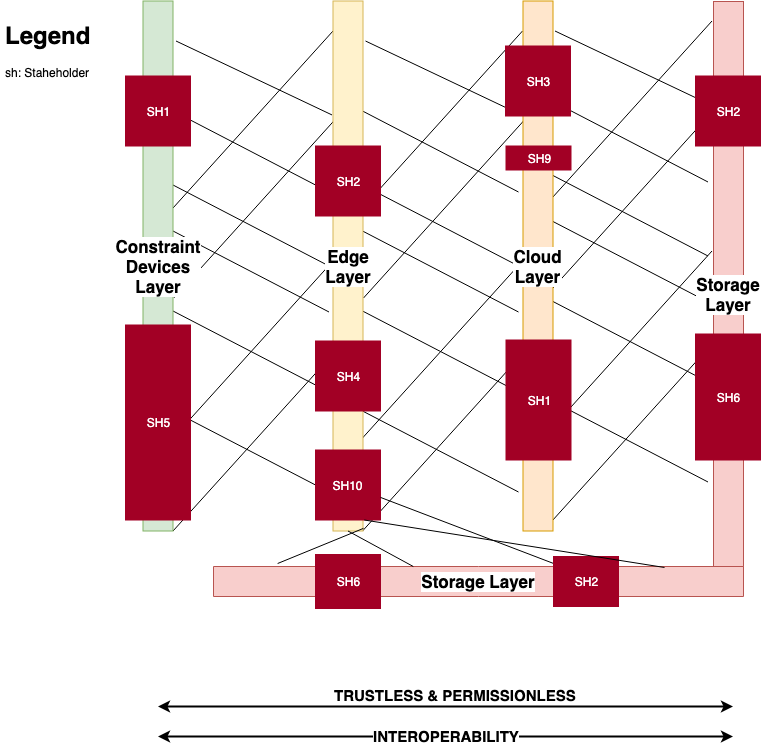
\includegraphics[width=0.9\textwidth]{images/layers_decentralized_v2.png}
    \caption{The IoT reference architecture as a series of decentralized networks that form it's layers}
    \label{fig:layers_decent}
\end{figure}


Figure \ref{fig:layers_decent} is similar to figure \ref{fig:layers_now} but features a completely decentralized model.

Each red box is the system that belongs to a different stakeholder, while the size of the boxes are proportional to the size of the infrastructure, qualitatively,

Each line models the Parent-Children relationship between subsystems of different layers. We demonstrate that \textit{any} constraint device can use \textit{any} edge device as a gateway and \textit{any} edge device can use \textit{any} cloud system as back-end. \textit{Any} is used in a qualitative manner as we are describing a dynamic market where demand \& offer will be determined by many different parameters. The devices, in any layer, have a set of parameters that forbid certain connections, the most prominent one being the connectivity protocol. It is apparent that a contraint device which exclusively supports Zigbee can not be managed by an IoT Edge that supports BLE (Blueetooth Low Energy) and LoRa.

We hope that our research will contribute towards the end goal of a decentralized IoT Edge computing System, where the interoperability will enable the democratization of the domain and the proliferation of IoT devices, by enabling any device to interface to any Edge or Cloud computing system. 

 \clearemptydoublepage

% Next Chapters
% .............
% .............

%**************************%
%    END OF MAIN THESIS    %
%**************************%

% bibliography
\bibliographystyle{unsrt}
\bibliography{library/bibliography.bib}
\clearemptydoublepage

% Last Page
\pagestyle{empty}

\vspace*{\fill}
\noindent \hspace{2cm} \rule{12.7cm}{0.4pt}\\
\vspace{-1.7em}
\begin{flushleft}
	\hspace*{30mm}University of Patras, Polytechnic School\\
	\hspace*{30mm}Department of Electrical Engineering \& Computer Technology\\
	\hspace*{30mm}{\nomme}\\
	\hspace*{30mm}© \monthyear \ -- All Rights Reserved\\
\end{flushleft}
\vspace{-1.2em}
\noindent \hspace{2cm} \rule{12.7cm}{0.4pt}

\end{document}
